\documentclass{report}
% Packages


\usepackage{mathpazo}
\usepackage[english]{babel}

\usepackage[T1]{fontenc}
\usepackage[utf8]{inputenc}

\usepackage{biblatex} 
\usepackage{geometry}
\geometry{margin=1.3in}
\usepackage{amsmath,amsfonts,amssymb,amsthm,mathrsfs}
\usepackage{extarrows}
\usepackage{csquotes}
\usepackage{pgf,tikz-cd}
\usetikzlibrary{babel}
\usepackage{hyperref}
\newtheorem{theo}{Theorem}
\newtheorem{prop}{Proposition}
\newtheorem{defi}{Definition}
\newtheorem{coro}{Corollary}
\newtheorem{lemm}{Lemma}
\newtheorem{example}{Example}
\newtheorem{fac}{Fact}
\newtheorem{rema}{Remark}
\newcommand{\ca}{$\mathcal{A}$ }
\newcommand{\cb}{$\mathcal{B}$ }
\newcommand{\cc}{$\mathcal{C}$ }
\newcommand{\cd}{$\mathcal{D}$ }
\renewcommand{\bf}[1]{\textbf{#1}}

% Title and Author
\title{PhD Studies}
\author{Abraham Rojas Vega}
\addbibresource{notas.bib} % Specify the path to your bibliography file


\begin{document}

\maketitle

\tableofcontents

\part{Topics of Algebra}

%\chapter{Foundations of Mathematics}

\chapter{Category Theory}

\textit{References \cite{adamekAbstractConcreteCategories2004,richterCategoriesHomotopyTheory2020}.}\\ %ritcher
In general, categories and functors will be denoted with calligraphic letters (except for Gr, Ab, Top, Sets, \dots) and objects with capital letters.\\

\section{Some facts}  

\begin{example}
    \begin{enumerate}
        \item On a topological space, the category of open sets with inclusions as morphisms. The opposite of this category, denoted by $\mathcal{U}$, is essential in sheaf theory.
        \item If \ca and \cb are preordered sets, then the functors between them are the monotone maps.
        \item $i: \mathbb{Z} \hookrightarrow \mathbb{Q}$ is a monomorphism and epimorphism, but not an isomorphism.
        \item A \textbf{grupoid} is a category with whose morphisms are isomorphisms. In particular, a group can be seen as a grupoid with one element.
    \end{enumerate}
\end{example}
\medspace

% A functor $F: \mathcal{A} \rightarrow \mathcal{B}$ is called an \textbf{isomorphism} provided that there is a functor $G: \mathcal{B} \rightarrow \mathcal{A}$ such that $G \circ F=i d_{\mathcal{A}}$ and $F \circ G=i d_{\mathcal{B}}$. The categories $\mathcal{A}$ and $\mathcal{B}$ are said to be \textbf{isomorphic}. \\
% Note that $G$ is uniquely determined by $F$. It will be denoted by $F^{-1}$ and called the \textbf{inverse} of $F$.\\

Let $F: \mathcal{A} \rightarrow \mathcal{B}$ be a functor.
\begin{enumerate}
    \item $F$ is \textbf{faithful} provided that all the \textbf{hom-set restrictions}
    $$
    F: \operatorname{hom}_{\mathcal{A}}\left(A, A^{\prime}\right) \rightarrow \operatorname{hom}_{\mathcal{B}}\left(F A, F A^{\prime}\right)
    $$
    are injective.
    \item $F$ is \textbf{full} if all hom-set restrictions are surjective.
    \item $F$ is an \textbf{embedding} if and it is faithful and injective on the class of objects.
    \item $F$ is \textbf{essentially surjective} if for every object $B$ of \cb, there is an object $A$ of \ca such that $F A$ is isomorphic to $B$. 
    \item If $F$ is essentially surjective and fully faithful, it is called an \textbf{equivalence of categories}, and \ca and \cb are said to be \textbf{equivalent}.
\end{enumerate}

Let $F, G: \mathcal{A} \rightarrow \mathcal{B}$ be functors. A \textbf{natural transformation} $\tau: F \rightarrow G$ is a function that assigns to each $\mathcal{A}$-object $A$ a $\mathcal{B}$-morphism $\tau_A: F A \rightarrow G A$ in such a way that the following \textit{natural} condition holds: for each A-morphism $A \xrightarrow{f} A^{\prime}$, the diagram
$
\begin{tikzcd}
FA \arrow[r, "\tau_A"] \arrow[d, "Ff"'] & GA \arrow[d, "Gf"] \\
FA' \arrow[r, "\tau_{A'}"'] & GA'
\end{tikzcd}
$ commutes.\\
A natural transformation $F \xrightarrow{\tau} G$ whose components $\tau_A$ are isomorphisms is called a \textbf{natural isomorphism} from $F$ to $G$, and $F$ and $G$ are said to be \textbf{naturally isomorphic}, denoted by $F \cong G$.

\begin{example}
    Consider the $n$-th singular homology group of a pair of spaces $(X, A)$. The long exact sequence of the pair contains the group morphisms
$$
\delta: H_n(X, A) \rightarrow H_{n-1}(A) .
$$
\noindent
This forms a natural transformation between $(X, A) \mapsto H_n(X, A)$ and $(X, A) \mapsto$ $H_{n-1}(A)$, both being from the category of pairs of topological spaces to the category of abelian groups. \\



    \begin{enumerate}
        %\item Let $U: \operatorname{Gr} \rightarrow \operatorname{Set} $ be the forgetful functor, and let $S: \operatorname{Grp} \rightarrow$ Set be the "squaring-functor", defined by $S(G \xrightarrow{f} H)=G^2 \xrightarrow{f^2} H^2$. For each group $G$, its multiplication is a function $\tau_G: G^2 \rightarrow G$. The family $\tau=\left(\tau_G\right)$ is a natural transformation from $S$ to $U$. The naturality condition simply means that $f(x \cdot y)=f(x) \cdot f(y)$ for any group homomorphism $G \xrightarrow{f} H$ and any $x, y \in G$. Thus "multiplication" in groups can be regarded as a natural transformation. Similar for other structures.
        %\item Let $(\,\hat{} \,):$ Vec $\rightarrow$ Vec be the second-dual functor for vector spaces, then $\tau_V: V \rightarrow \hat{\hat{V}}$, defined by $\left(\tau_V(x)\right)(f)=f(x)$, yield a natural transformation $i d{ }_{\mathrm{Vec}} \xrightarrow{\tau}(\,\hat{}\,)$. It becomes a natural isomorphism when restricted to finite-dimensional vector spaces.
        \item The assignment of the Hurewicz homomorphism $\pi_n(X) \rightarrow H_n(X)$ to each topological space $X$ is a natural transformation.
        \item If $B \xrightarrow{f} C$ is an $\mathcal{A}$-morphism, then
        $
        \operatorname{hom}_{\mathcal{A}}(C,-) \xrightarrow{\tau_f} \operatorname{hom}_{\mathcal{A}}(B,-),
        $
        defined by $\tau_f(g)=g \circ f$, and
        $
        \operatorname{hom}_{\mathcal{A}}(-, B) \xrightarrow{\sigma_f} \operatorname{hom}_{\mathcal{A}}(-, C) \text {, }
        $
        defined by $\sigma_f(g)=f \circ g$, are natural transformations.
        \item (Good definitions of extension) Let $F:$ Set $\rightarrow$ Vec be a functor that assigns to each set $X$ a vector space $F X$ with basis $X$, and to each function $X \xrightarrow{f} Y$ the unique linear extension $F X \xrightarrow{F f} F Y$ of $f$. This actually is not a correct definition of a functor, since there are many different vector spaces with the same basis. However, the definition is "correct up to natural isomorphism". Whenever we choose, for each set $X$, a specific vector space $F X$ with basis $X$, we do obtain a functor $F:$ Set $\rightarrow$ Vec (since the above condition determines the action of $F$ on functions uniquely). Furthermore, any two functors that are obtained in this way are naturally isomorphic.
%        \item For any 2-element set $A$, hom $(A,-)$ is naturally isomorphic to the squaring functor $S^2[3.20(10)]$ and hom $(-, A)$ is naturally isomorphic to the contravariant power-set functor $\mathcal{Q}[3.20(9)]$. If $B$ is isomorphic to $A$, then hom $(A,-)$ and hom $(B,-)$ are naturally isomorphic with those functors, the converse is true.
    \end{enumerate}
\end{example}






\section{Limits and colimits}

An object $P$ in a category $\mathcal{C}$ is called \textbf{projective} if, for every epimorphism $f: M \rightarrow Q$ in $\mathcal{C}$ and every $p: P \rightarrow Q$, there is a $\xi \in \operatorname{Hom}(P, M)$ with $f \circ \xi=p$, called the \textbf{lift} of $p$ to $M$.\\
Dually, an object $I$ in a category $\mathcal{C}$ is called \textbf{injective} if for every monomorphism $f: U \rightarrow M$ in $\mathcal{C}$ and every $j: U \rightarrow I$, there is a $\zeta \in \operatorname{Hom}(M, I)$ with $\zeta \circ f=j$, called and \textbf{extension} of $j$ to $M$.\\
\medspace


\tikzset{every picture/.style={line width=0.75pt}} %set default line width to 0.75pt        

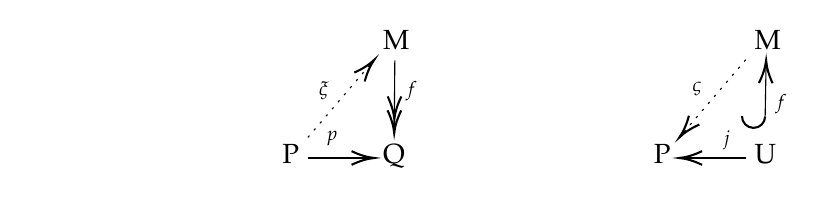
\begin{tikzpicture}[x=0.75pt,y=0.75pt,yscale=-1,xscale=1]
%uncomment if require: 
\path (0,81); %set diagram left start at 0, and has height of 81


% Text Node
\draw (132,62) node [anchor=north east] [inner sep=0.75pt]   [align=left] {P};
% Text Node
\draw (169.99,62) node [anchor=north west][inner sep=0.75pt]   [align=left] {Q};
% Text Node
\draw (169.99,19) node [anchor=south west] [inner sep=0.75pt]   [align=left] {M};
% Text Node
\draw (139,32) node [anchor=north west][inner sep=0.75pt]  [font=\scriptsize] [align=left] {$\displaystyle \xi $};
% Text Node
\draw (319,32) node [anchor=north west][inner sep=0.75pt]  [font=\scriptsize] [align=left] {$\displaystyle \varsigma $};
% Text Node
\draw (181,32) node [anchor=north west][inner sep=0.75pt]  [font=\scriptsize] [align=left] {$\displaystyle f$};
% Text Node
\draw (359,38) node [anchor=north west][inner sep=0.75pt]  [font=\scriptsize] [align=left] {$\displaystyle f$};
% Text Node
\draw (142.6,55.6) node [anchor=north west][inner sep=0.75pt]  [font=\scriptsize] [align=left] {$\displaystyle p$};
% Text Node
\draw (336.78,55.6) node [anchor=north] [inner sep=0.75pt]  [font=\scriptsize] [align=left] {$\displaystyle j$};
% Text Node
\draw (310.99,62) node [anchor=north east] [inner sep=0.75pt]   [align=left] {P};
% Text Node
\draw (348.98,62) node [anchor=north west][inner sep=0.75pt]   [align=left] {U};
% Text Node
\draw (348.98,19) node [anchor=south west] [inner sep=0.75pt]   [align=left] {M};
% Connection
\draw    (176.89,23) -- (176.59,58) ;
\draw [shift={(176.59,58)}, rotate = 270.49] [color={rgb, 255:red, 0; green, 0; blue, 0 }  ][line width=0.75]    (17.64,-3.29) .. controls (13.66,-1.4) and (10.02,-0.3) .. (6.71,0) .. controls (10.02,0.3) and (13.66,1.4) .. (17.64,3.29)(10.93,-3.29) .. controls (6.95,-1.4) and (3.31,-0.3) .. (0,0) .. controls (3.31,0.3) and (6.95,1.4) .. (10.93,3.29)   ;
% Connection
\draw  [dash pattern={on 0.84pt off 2.51pt}]  (135,60.07) -- (165.69,24.2) ;
\draw [shift={(166.99,22.68)}, rotate = 130.56] [color={rgb, 255:red, 0; green, 0; blue, 0 }  ][line width=0.75]    (10.93,-3.29) .. controls (6.95,-1.4) and (3.31,-0.3) .. (0,0) .. controls (3.31,0.3) and (6.95,1.4) .. (10.93,3.29)   ;
% Connection
\draw    (135,70) -- (164.99,70) ;
\draw [shift={(166.99,70)}, rotate = 180] [color={rgb, 255:red, 0; green, 0; blue, 0 }  ][line width=0.75]    (10.93,-3.29) .. controls (6.95,-1.4) and (3.31,-0.3) .. (0,0) .. controls (3.31,0.3) and (6.95,1.4) .. (10.93,3.29)   ;
% Connection
\draw    (315.99,70) -- (345.98,70) ;
\draw [shift={(313.99,70)}, rotate = 0] [color={rgb, 255:red, 0; green, 0; blue, 0 }  ][line width=0.75]    (10.93,-3.29) .. controls (6.95,-1.4) and (3.31,-0.3) .. (0,0) .. controls (3.31,0.3) and (6.95,1.4) .. (10.93,3.29)   ;
% Connection
\draw    (355.32,50) -- (355.75,25) ;
\draw [shift={(355.78,23)}, rotate = 90.97] [color={rgb, 255:red, 0; green, 0; blue, 0 }  ][line width=0.75]    (10.93,-3.29) .. controls (6.95,-1.4) and (3.31,-0.3) .. (0,0) .. controls (3.31,0.3) and (6.95,1.4) .. (10.93,3.29)   ;
\draw [shift={(355.32,50)}, rotate = 270.97] [color={rgb, 255:red, 0; green, 0; blue, 0 }  ][line width=0.75]      (0,-11.18) .. controls (-3.09,-11.18) and (-5.59,-8.68) .. (-5.59,-5.59) .. controls (-5.59,-2.5) and (-3.09,0) .. (0,0) ;
% Connection
\draw  [dash pattern={on 0.84pt off 2.51pt}]  (345.98,22.68) -- (315.29,58.55) ;
\draw [shift={(313.99,60.07)}, rotate = 310.56] [color={rgb, 255:red, 0; green, 0; blue, 0 }  ][line width=0.75]    (10.93,-3.29) .. controls (6.95,-1.4) and (3.31,-0.3) .. (0,0) .. controls (3.31,0.3) and (6.95,1.4) .. (10.93,3.29)   ;

\end{tikzpicture}

%$\mathcal{C}$ with $[0], \mathcal{C} *[0]$, has 0 as a terminal object and that $[0] * \mathcal{C}$ has 0 as an initial object. The category $\mathcal{C} *[0]$ is the \textbf{inductive cone} with base $\mathcal{C}$, and [0]* $\mathcal{C}$ is the \textbf{projective cone} with base $\mathcal{C}$.



\begin{example}
    \begin{enumerate}
        \item In $\operatorname{Sets}$, every object is injective and projective.
        \item In $R-\operatorname{Mod}$ (left), a module is projective iff it is a direct summand of a free module. A module $M$ is injective if and only if the functor $\operatorname{Hom}_R(-, M)$ is exact.
        %\item An abelian group $A$ is a \textbf{divisible ableian group} if $nA= A$ for every $n \in \mathbb{N}$. Every divisible abelian group is an injective $\mathbb{Z}$-module, an viceversa. 
    \end{enumerate}
\end{example}

\begin{prop}
\begin{enumerate}
    %\item If $P$ is a projective object of a category $\mathcal{C}$ and if $i: U \rightarrow P$ is a monomorphism in $\mathcal{C}$ with a retraction $r: P \rightarrow U$, then $U$ is projective. Similarly, if $i: J \rightarrow I$ is a monomorphism with retraction $r: I \rightarrow J$ and $I$ is injective, then $J$ is injective.    
    %\item If $q: Q \rightarrow P$ is an epimorphism and if $P$ is projective, then $q$ has a section. Dually, if $j: I \rightarrow J$ is a monomorphism and $I$ is injective, then $j$ has a retraction.
    \item $A$ is projective if and only if $\operatorname{Hom}_\mathcal{C}(A,-): \mathcal{C} \rightarrow$ Sets preserves epimorphisms. 
    \item $A$ is injective if and only if $\operatorname{Hom}_\mathcal{C}(-, A): \mathcal{C}^o \rightarrow$ Sets sends monomorphisms to epimorphisms.
\end{enumerate}
\end{prop}




Let $A \stackrel{\text { f }}{\underset{g}{\rightrightarrows}} B$ be a pair of morphisms. A morphism $E \xrightarrow{e} A$ is called an \textbf{equalizer} of $f$ and $g$ provided that the following conditions hold:
(1) $f \circ e=g \circ e$,
(2) for any morphism $e^{\prime}: E^{\prime} \rightarrow A$ with $f \circ e^{\prime}=g \circ e^{\prime}$, there exists a unique morphism $\bar{e}: E^{\prime} \rightarrow E$ such that $e^{\prime}=e \circ \bar{e}$, i.e., such that the triangle
\begin{tikzcd}
    E' \arrow[d, "\overline{e}"'] \arrow[dr, "e'"] & \\
    E \arrow[r, "e"'] & A \arrow[r, shift left, "f"] \arrow[r, shift right, "g"'] & B
    \end{tikzcd} commutes.\\

   

A \textbf{source} is a pair $\left(A,\left(f_i\right)_{i \in I}\right)$ consisting of an object $A$ and a family of morphisms $f_i: A \rightarrow A_i$ with domain $A$, indexed by some class $I$.\\
A source $\mathcal{P}=\left(P \xrightarrow{p_i} A_i\right)_I$ is called a \textbf{product} provided that for every source $\mathcal{S}=$ $\left(A \xrightarrow{f_i} A_i\right)_I$ with the same codomain as $\mathcal{P}$ there exists a unique morphism $A \xrightarrow{f} P$ with $\mathcal{S}=\mathcal{P} \circ f$. A product with codomain $\left(A_i\right)_I$ is called a \textbf{product of the family} $\left(A_i\right)_I$.\\

%\begin{fac}
 %   A category has finite products if and only if it has terminal objects and products of pairs of objects.
  %  A category that has products for all class-indexed families must be thin.
%A small category has products if and only if it is equivalent to a complete lattice.
%\end{fac}
 A \textbf{diagram} in a category $\mathcal{A}$ is a functor $D: \mathbf{I} \rightarrow \mathcal{A}$, where $\mathbf{I}$ is called the \textbf{scheme} of the diagram. A diagram with a small (or finite) scheme is said to be \textbf{small} (or finite).\\
An A-source $\left(A \xrightarrow{f_i} D_i\right)_{i \in O b(\mathrm{I})}$ is said to be \textbf{natural} for the diagram $D$ provided that for each I-morphism $i \xrightarrow{d} j$, the triangle 
\begin{tikzcd}
    A \arrow[d, "f_i"'] \arrow[dr, "f_j"] & \\
    D_i \arrow[r, "Dd"'] & D_j 
\end{tikzcd} commutes. Equivalently, natural sources can be regarded as natural transformations from constant functors $C: \mathbf{I} \rightarrow \mathbf{A}$ to the functor $D$.\\
A \textbf{limit} of a diagram $D$ is a natural source $\left(L \xrightarrow{\ell_i} D_i\right)$ for $D$ with the \textbf{universal property} that for each natural source $\left(A \xrightarrow{f_i} D_i\right)$ there exists a unique morphism $f: A \rightarrow L$ with $f_i=$ $\ell_i \circ f$ for each $i \in O b(\mathbf{I})$.\\
 A poset $\mathbf{I}$ is \textbf{down-directed} if every pair of elements has a lower bound. Limits of diagrams with this king of scheme are called \textbf{projective} (or \textbf{inverse}) limits. 


\begin{prop}
    
\begin{enumerate}
%    \item Every source is natural for a diagram with discrete scheme. Products are limits of diagrams with discrete scheme. An object, considered as an empty source, is a limit of the empty diagram if and only if it is a terminal object.

    \item For A-morphisms $A \underset{g}{\stackrel{f}{\rightrightarrows}} B$, considered as a diagram $D$ with scheme $\bullet \Rightarrow \bullet$, a source $(A \stackrel{e}{\longleftarrow} C \xrightarrow{h} B)$ is natural provided that $g \circ e=h=f \circ e$.\\
    $C \xrightarrow{e} A$ is an equalizer of $A \xrightarrow[g]{\stackrel{f}{\longrightarrow}} B$ if and only if the source $(A \stackrel{e}{\leftarrow} C \xrightarrow{f \circ e} B)$ is a limit of $D$. 
\end{enumerate}
\end{prop}

\begin{prop}[Uniqueness]
If $\mathcal{L}=\left(L \xrightarrow{\ell_i} D_i\right)_{i \in O b(\mathbf{I})}$ is a limit of $D: \mathbf{I} \rightarrow \mathbf{A}$, then
    \begin{enumerate}
        \item for each limit $\mathcal{K}=\left(K \xrightarrow{k_i} D_i\right)_{i \in O b(\mathrm{I})}$ of $D$, there exist an isomorphism $K \xrightarrow{h} L$ with $\mathcal{K}=\mathcal{L} \circ h$,
        \item for each isomorphism $A \xrightarrow{h} L$, the source $\mathcal{L} \circ h$ is a limit of $D$.
    \end{enumerate}
\end{prop}

%cone over a limit (Ritcher)
% cambio de notacion, no se mencionan diagramas

%\begin{prop}
%If $G: \mathcal{D} \rightarrow \mathcal{C}$ is another functor and if $\alpha: F \Rightarrow G$ is a natural transformation, then $\alpha$ induces a morphism $\operatorname{colim}_{\mathcal{D}} \alpha \in \mathcal{C}\left(\operatorname{colim}_D F, \operatorname{colim}_{\mathcal{D}} G\right)$. Prove that this turns $\operatorname{colim}_{\mathcal{D}}$ into a functor from $\operatorname{Fun}(\mathcal{D}, \mathcal{C})$ to $\mathcal{C}$.    
%\end{prop}

%\begin{prop}
%If the colimit ($\operatorname{colim}_{\mathcal{D}} F, \tau$) exists for all functors $F: \mathcal{D} \rightarrow \mathcal{C}$, then the functor $\operatorname{colim}_{\mathcal{D}}: \operatorname{Fun}(\mathcal{D}, \mathcal{C}) \rightarrow \mathcal{C}$ is left adjoint to the diagonal functor $\Delta: \mathcal{C} \rightarrow \operatorname{Fun}(\mathcal{D}, \mathcal{C})$, that is, there are natural isomorphisms
%$$\mathcal{C}\left(\operatorname{colim}_{\mathcal{D}} F, C\right) \cong \operatorname{Fun}(\mathcal{D}, \mathcal{C})(F, \Delta(C))$$for all functors $F$ and all object $C$ of $\mathcal{C}$.
%\end{prop}


\begin{example}[Limits]
    \begin{enumerate}
        \item Let $\left(X_n\right)_{n \in \mathbb{N}_0}$ be a family of sets with $X_{n+1} \subset X_n$. Then, the limit of the system
        $
        \ldots \subset X_{n+1} \subset X_n \subset \ldots \subset X_1 \subset X_0
        $
        is the intersection of the sets $X_n$.
        \item Let $p$ be a fixed prime. The inverse limit of the diagram
        is the ring of $p$-adic integers, $\mathbb{Z}_p$. Here, the maps $p_i$ are the canonical projection maps. An explicit model of the limit is
        $$
        \left\{\left(x_1, x_2, x_3, \ldots\right) \in \prod_{n \geq 1} \mathbb{Z} / p^n \mathbb{Z} \mid p_i\left(x_i\right)=x_{i-1} \text { for all } i \geq 2\right\} .
        $$
        This carries a ring structure, where addition and multiplication are defined coordinatewise.
        \item Kernels in the category of abelian groups are limits of diagrams of the form $A \underset{f}{\stackrel{0}{\longrightarrow}} B$.
        \item The presheaf $F$ is a sheaf if for every $U \in \mathfrak{U}(X)$ and for every open covering $\left(U_i\right)_{i \in I}$ of $U$, the following diagram is an equalizer:
        $$
        F(U) \longrightarrow \prod_{i \in I} F\left(U_i\right) \Longrightarrow \prod_{i, j \in I} F\left(U_i \cap U_j\right) .
        $$
        
        Here, the first map is induced by the restriction maps res $U_U^{U_i}$, and the second pair of arrows is induced by two sets of restriction maps. $U_i \cap U_j$ is a subset of $U_i$ and of $U_j$.
        Sheaves form a category as a full subcategory of the category of presheaves.
        \item Fiber products in the category of sets are limits of diagrams of the form $A \underset{f}{\stackrel{g}{\longrightarrow}} C$. A concrete model for this pullback in these categories is $$f^*(p):=Z \times_Y X:=\{(z, x) \in Z \times X \mid f(z)=p(x)\}$$
    \end{enumerate}
\end{example}


Dually (inverting the arrow) we define colimit, coproducts, coequalizers...\\
%definicion dual de colimite

If you build the colimit over a discrete diagram category (small category $\mathcal{D}$ that has only identity morphisms), then the colimit of a functor $F: \mathcal{D} \rightarrow \mathcal{C}$ is called the \textbf{coproduct} of the $F(D)$ for $D$ an object of $\mathcal{D}$, denoted by
        $
        \bigsqcup_{\mathcal{D}} F(D) .
        $
        Coproducts in the category of sets and in the category of topological spaces are the disjoint unions.
        Every coproduct comes with canonical structure maps, called \textbf{inclusions}.\\
\textbf{Pushouts} are colimits over a diagram category $\mathcal{D}$ of the form
        $
        D_1 \leftarrow D_0 \rightarrow D_2 .
        $.\\
Another important class of examples is \textbf{coequalizers}. These are colimits of diagrams of the form
        $
        F\left(D_0\right) \underset{\alpha}{\stackrel{\beta}{\Longrightarrow}} F\left(D_1\right) .
        $


\begin{example}[Colimits]
    \begin{enumerate}
        \item Colimits exist in the category of Sets:
        $$
        \operatorname{colim}_{\mathcal{D}} F=\bigsqcup_{D \text { object of } \mathcal{D}} F(D) / \sim,
        $$
        where we declare that an $x \in F(D)$ is equivalent to a $y \in F\left(D^{\prime}\right)$ if there is a morphism $f \in \mathcal{D}\left(D, D^{\prime}\right)$, such that $F(f)(x)=y$. This relation is not symmetric, so one has to consider the equivalence relation generated by this relation. 
        \item If all structure maps $F(i<j)$ are monomorphisms, then we might interpret the colimit $\operatorname{colim}_{\mathcal{D}} F$ as the union of the $F(i)$ s. Typical examples are increasing sequences of sets or topological spaces
        $$
        X_0 \subset X_1 \subset X_2 \subset \ldots
        $$
        or increasing sequences of abelian groups, vector spaces, and other algebraic objects. 
        \item An important class of examples is CW complexes. These are the colimits of their skeleta.
        \item In stable homotopy theory, the stable homotopy groups of spheres are a central object of study. Let $\mathbb{S}^n$ denote the unit sphere in $\mathbb{R}^{n+1}$. As the smash product of spheres satisfies $\mathbb{S}^1 \wedge \mathbb{S}^n \cong \mathbb{S}^{n+1}$ we have stabilization maps
        $$
        \pi_n\left(\mathbb{S}^m\right)=\left[\mathbb{S}^n, \mathbb{S}^{m+1}\right]_* \rightarrow\left[\mathbb{S}^{n+1}, \mathbb{S}^{m+1}\right]_*=\pi_{n+1}\left(\mathbb{S}^m\right)
        $$
        that send a homotopy class $[f]$ to the homotopy class of $\mathbb{S}^1 \wedge f$. Therefore, for every $m$, we get a sequential colimit and as $\pi_n\left(\mathbb{S}^m\right)=0$ for $n<m$, we can express $\pi_n\left(\mathbb{S}^m\right)$ as $\pi_{k+m}\left(\mathbb{S}^m\right)$ in the nontrivial cases, with $k \geq 0$, and get the $k$ th stable homotopy group of spheres as
        $$
        \pi_k^s=\operatorname{colim}\left(\pi_{k+m}\left(\mathbb{S}^m\right) \rightarrow \pi_{k+m+1}\left(\mathbb{S}^{m+1}\right) \rightarrow \pi_{k+m+2}\left(\mathbb{S}^{m+2}\right) \rightarrow \ldots\right)
        $$
        \item The first groups are $\pi_0^s=\mathbb{Z}, \pi_1^s=\mathbb{Z} / 2 \mathbb{Z}$ generated by the stabilization of the Hopf $\operatorname{map} \eta: \mathbb{S}^3 \rightarrow \mathbb{S}^2, \pi_2^s=\mathbb{Z} / 2 \mathbb{Z}, \pi_3^s=\mathbb{Z} / 24 \mathbb{Z}$, and so on.
        \item In the category of pointed topological spaces the pointed sum (also known as the bouquet of spaces) is the coproduct.
        \item Coproducts in the category of abelian groups are given by the direct sum. Coproducts in the category of general groups is the free product.
        \item If $A$ is a topological space, together with continuous maps $f: A \rightarrow X$ and $g: A \rightarrow Y$, the pushout of $X \leftarrow A \rightarrow Y$ is the quotient space of the disjoint union $X \sqcup Y$ by the equivalence relation that identifies $f(a)$ with $g(a)$ for all $a \in A$.
        \item Pushouts of groups are given by amalgamated products, given by $G_1 *_{G_0} G_2$, which is the quotient of the free product $G_1 * G_2$ by the normal subgroup generated by words of the form $f\left(g_0\right) h\left(g_0\right)^{-1}$ for $g_0 \in G_0$.
        \item The cokernel of a homomorphism $f$ is the coequalizer of the diagram $A \underset{f}{\stackrel{0 }{\longrightarrow}} B$ in the category Ab.
    \end{enumerate}
\end{example}




\section{Adjoint functors}

Let $\mathcal{C}$ and $\mathcal{C}^{\prime}$ be categories. An \textbf{adjunction} between $\mathcal{C}$ and $\mathcal{C}^{\prime}$ is a pair of functors $L: \mathcal{C} \rightarrow \mathcal{C}^{\prime}, R: \mathcal{C}^{\prime} \rightarrow \mathcal{C}$, such that for each pair of objects $C$ of $\mathcal{C}$ and $C^{\prime}$ of $\mathcal{C}^{\prime}$, there is a bijection of sets
$$
\varphi_{C, C^{\prime}}: \mathcal{C}^{\prime}\left(L(C), C^{\prime}\right) \cong \mathcal{C}\left(C, R\left(C^{\prime}\right)\right),
$$
which is natural in $C$ and $C^{\prime}$.
The functor $L$ is then left adjoint to $R$, and $R$ is right adjoint to $L$. We call $(L, R)$ an adjoint pair of functors.\\
The naturality condition on the bijections $\varphi_{C, C^{\prime}}$ can be spelled out explicitly as follows: For all morphisms $f: C \rightarrow D$ in $\mathcal{C}$ and $g: C^{\prime} \rightarrow D^{\prime}$ in $\mathcal{C}^{\prime}$, the diagram commutes.

\begin{center}
    

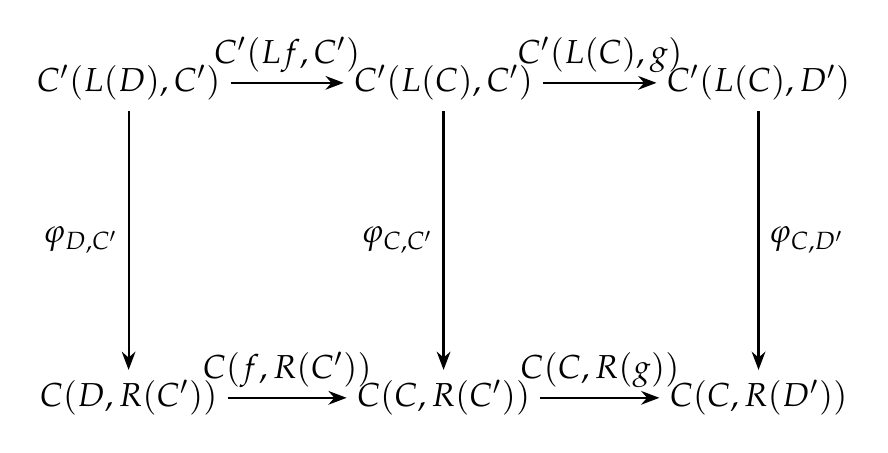
\begin{tikzpicture}[  > = Stealth,  node distance = 4cm,  auto,  thick,  font = \large\itshape]
  % Define nodes
  \node (A) {$C'(L(D), C')$};
  \node (B) [right of=A] {$C'(L(C), C')$};
  \node (C) [right of=B] {$C'(L(C), D')$};
  \node (D) [below of=A] {$C(D, R(C'))$};
  \node (E) [below of=B] {$C(C, R(C'))$};
  \node (F) [below of=C] {$C(C, R(D'))$};
  
  % Draw arrows
  \draw[->] (A) -- node[above] {$C'(Lf,C')$} (B);
  \draw[->] (B) -- node[above] {$C'(L(C),g)$} (C);
  \draw[->] (D) -- node[above] {$C(f,R(C'))$} (E);
  \draw[->] (E) -- node[above] {$C(C,R(g))$} (F);
  \draw[->] (A) -- node[left] {$\varphi_{D,C'}$} (D);
  \draw[->] (B) -- node[left] {$\varphi_{C,C'}$} (E);
  \draw[->] (C) -- node[right] {$\varphi_{C,D'}$} (F);
\end{tikzpicture}
\end{center}

\begin{example}
A prototypical example of an adjunction is a forgetful functor and a 'free' functor: if $R=U$ is a forgetful functor and if a left adjoint of $U$ exists, then the defining property means that for each morphism from $C$ to $U\left(C^{\prime}\right)$ in the underlying category, there is a unique corresponding morphism from $L(C)$ to $C^{\prime}$, so, in this sense, $L(C)$ is the free object associated with $C$. For topological spaces, the free topological space on a set is the set with discrete topology.
\end{example}

\begin{prop}
    \begin{enumerate}
      \item The functor $L$ is left adjoint to $R$ iff there are natural transformations $\eta$ : Id $\Rightarrow R \circ L$ and $\varepsilon: L \circ R \Rightarrow$ Id with the properties that
      $$
      \varepsilon_L \circ L(\eta)=\operatorname{Id}_L \text { and } R(\varepsilon) \circ \eta_R=\operatorname{Id}_R
      $$
      hence, the diagrams
      $$
      L(C) \xrightarrow{L(\eta)} L R L(C) \text { and } R\left(C^{\prime}\right) \xrightarrow{\eta_{R\left(C^{\prime}\right)}} R L R\left(C^{\prime}\right)
      $$
      commute for all objects $C$ of $\mathcal{C}$ and $C^{\prime \prime}$ of $\mathcal{C}^{\prime}$.
      \item Adjunction can be composed.
      \item Each of the functors $L$ and $R$ determines the other functor uniquely up to isomorphism.
      \item $G$ has a left-adjoint $F$ if and only if $\operatorname{Hom}_C(X, G-)$ is representable for all $X$ in $C$. The natural isomorphism $\Phi_X: \operatorname{Hom}_D(F X,-) \rightarrow \operatorname{Hom}_C(X, G-)$ yields the adjointness; that is
$$
\Phi_{X, Y}: \operatorname{Hom}_{\mathcal{D}}(F X, Y) \rightarrow \operatorname{Hom}_{\mathcal{C}}(X, G Y)
$$
is a bijection for all $X$ and $Y$.
    \end{enumerate}
\end{prop}
The transformation $\eta$ is called the \textbf{unit of the adjunction} and $\varepsilon$ is the \textbf{counit}.

%%%%% adicionar sobre diagramas refelectivos!!!!

\begin{theo}
Let $F: \mathcal{C} \rightarrow \mathcal{D}$ be an arbitrary functor. Then the following are equivalent.
\begin{enumerate}
    \item The functor $F$ possesses a left adjoint $L$, and the corresponding natural transformations $\varepsilon: L F \Rightarrow \operatorname{Id}$ and $\eta$ : Id $\Rightarrow F L$ are natural isomorphisms.
    \item There is a functor $L: \mathcal{D} \rightarrow \mathcal{C}$ and two arbitrary natural isomorphisms $\mathrm{Id} \cong F L$ and $L F \cong \mathrm{Id}$.
    \item The functor $F$ is fully faithful and essentially surjective.
\end{enumerate}
\end{theo}

\subsubsection*{Skeleta of categories}
 A category is called \textbf{reduced} if isomorphic objects are identical. A subcategory $\mathcal{S}$ of a category $\mathcal{C}$ is a \textbf{skeleton} if $\mathcal{S}$ is reduced and if the inclusion $\mathcal{S} \hookrightarrow \mathcal{C}$ is an equivalence of categories.
\begin{example}
    
    \begin{enumerate}
        
        \item Consider the category of finite sets and functions. It contains the full subcategory whose objects are the sets of the form $\{1, \ldots, n\}$ for $n \geq 0$. Here, we use the convention that the empty set is encoded by $n=0$. The inclusion functor is full and faithful. As every finite set is in bijection with a standardized set of the form $\{1, \ldots, n\}$ as above, the inclusion functor is also essentially surjective. Therefore, these finite sets build a skeleton.
        
        \item A similar example is the category of finite-dimensional $K$-vector spaces. This has as a skeleton the full subcategory of vector spaces of the form $K^n$ for some finite natural number $n$. Here, $n=0$ encodes the zero vector space.
    \end{enumerate}
\end{example}


\begin{prop}
    Every category has an skeleton
\end{prop}





\section{Concrete categories and representable functors}

A way to talk of \textit{low level structures} present on the objects of a category. Often it is easier to work with less structures, and there results like Yoneda's lemma that show us that it is possible to restrict our study to them.\\

Let \cc be a category. A \textbf{concrete category} over \cc is a category $\mathcal{A}$ together wih a faithful functor $U: \mathcal{A} \rightarrow \mathcal{C}$, called the \textbf{forgetful} (or underlying) functor of the concrete category. $\mathcal{C}$ is called the \textbf{base category}. A concrete category over Set is called a \textbf{construct}.\\
The category of groups (or topological spaces, rings, etc.), with the forgetful functor to Set, is a construct.\\

\begin{enumerate}
    \item A \textbf{structured arrow} with domain $X$ is a pair $(f, A)$ consisting of an A-object $A$ and an X-morphism $X \xrightarrow{f}|A|$,
    \item if $(f, A)$ is \textbf{generating} provided that for any pair of A-morphisms $r, s: A \rightarrow B$ the equality $r \circ f=s \circ f$ implies that $r=s$,
    \item and this $(f, A)$ is called \textbf{extremally generating} (resp. \textbf{concretely generating}) provided that each A-monomorphism (resp. A-embedding) $m: A^{\prime} \rightarrow A$, through which $f$ factors (i.e., $f=m \circ g$ for some $\mathbf{X}$-morphism $g$ ), is an $\mathbf{A}$-isomorphism.
    \item In a construct, an object $A$ is (extremally resp. concretely) generated by a subset $X$ of $|A|$ provided that the inclusion map $X \hookrightarrow|A|$ is (extremally resp. concretely) generating.
\end{enumerate}

\begin{prop}
    In a concrete category $\mathbf{A}$ over $\mathbf{X}$ the following hold for each structured arrow $f: X \rightarrow|A|:$
    \begin{enumerate}
        \item If $(f, A)$ is extremally generating, then $(f, A)$ is concretely generating.
        \item If $(f, A)$ is concretely generating, then $(f, A)$ is generating.
        \item If $X \xrightarrow{f}|A|$ is an $\mathbf{X}$-epimorphism, then $(f, A)$ is generating.
        \item If $X \xrightarrow{f}|A|$ is an extremal epimorphism in $\mathbf{X}$, and if $||$ preserves monomorphisms, then $(f, A)$ is extremally generating.
    \end{enumerate}
\end{prop}

\begin{example}
    \begin{enumerate}
        \item If an abstract category $\mathbf{A}$ is considered to be concrete over itself via the identity functor, then an A-morphism $A \xrightarrow{f} B$, considered as a structured arrow $(f, B)$, is generating (resp. extremally or concretely generating) if and only if $f$ is an epimorphism (resp. an extremal epimorphism). That is,
        $$
        \operatorname{Gen}(\mathbf{A})=\operatorname{Epi}(\mathbf{A}) \text { and } \operatorname{ExtrGen}(\mathbf{A})=\operatorname{ConcGen}(\mathbf{A})=\operatorname{ExtrEpi}(\mathbf{A})
        $$
        \begin{enumerate}
            \item In Vec, Grp, Sgr, Rng, and other algebraic constructs, the concepts of concrete generation and of extremal generation coincide with the familiar (non-categorical) concept of generation.
            In the constructs Sgr and Rng the inclusion map $\mathbb{Z} \hookrightarrow \mathbb{Q}$ is generating, but is not concretely generating [cf. 7.40(5)].

            \item In the construct $\mathbf{A}=$ Top we have
            $$
            \begin{aligned}
            & \text { ConcGen(A) }=\operatorname{Gen}(\mathbf{A})=\text { Surjective maps, and } \\
            & \operatorname{ExtrGen}(\mathbf{A})=\text { Surjective maps with discrete codomain. }
            \end{aligned}
            $$

            \item In the construct $\mathbf{A}=$ Haus we have
            $$
            \begin{aligned}
            \operatorname{Gen}(\mathbf{A}) & =\text { Dense maps } \\
            \text { ConcGen(A) } & =\text { Surjective maps, and } \\
            \text { ExtrGen(A) } & =\text { Surjective maps with discrete codomain. }
            \end{aligned}
            $$
        \item $A \xrightarrow{f} B$ is an epimorphism if and only if $(f, B)$ is generating.
\item If $(f, B)$ is extremally generating and the forgetful functor preserves monomorphisms, then $A \xrightarrow{f} B$ is an extremal epimorphism.
\item If $A \xrightarrow{f} B$ is an extremal epimorphism, then $(f, B)$ is concretely generating.    
        \end{enumerate}
    \end{enumerate}
\end{example}

A \textbf{universal arrow} over an $\mathbf{X}$-object $X$ is a structured arrow $X \xrightarrow{u}|A|$ with domain $X$ such that, for each structured arrow $X \xrightarrow{f}|B|$ with domain $X$, there exists a unique $A$-morphism $\hat{f}: A \rightarrow B$ such that the triangle 
\begin{tikzcd}
    X \arrow[r, "u"] \arrow[dr, "f"'] &  {|A|} \arrow[d, "\overline{f}"]\\
    & {|B|} 
\end{tikzcd} commutes. The pair $(u,A)$ is called a \textbf{free object}.

\begin{example}
\begin{enumerate}
    \item In a construct, an object $A$ is a free object over the empty set if and only if $A$ is an initial object, and over a singleton set if and only if $A$ represents the forgetful functor.
    \item In the construct Vec each object is a free object over any basis for it.
    \item In the constructs Top and Pos the free objects are precisely the discrete ones.
    \item In the construct $\mathbf{A b}$ free objects over $X$ are the free abelian groups generated by $X$.
    Similarly, the familiar free group generated by a set $X$ is a free object over $X$ in the construct Grp.
    \item To construct a universal arrow in (Ban, $O$ ) over a set $X$, let $\ell_1(X)$ be the subspace of the vector space $K^X$ consisting of all $r=\left(r_x\right)_{x \in X}$ in $K^X$ whose norm $\|r\|=$ $\sum_{x \in X}\left|r_x\right|$ is finite. Then $\ell_1(X)$ is a Banach space. Define $X \xrightarrow{u} O\left(\ell_1(X)\right)$ at $y$ by the Dirac function $u(y)=\left(\delta_{y x}\right)_{x \in X}$. Then $\left(u, \ell_1(X)\right)$ is a universal arrow over $X$. Observe, for comparison, that for the construct (Ban, $U$ ) the only set having a universal arrow is the empty set, and that for the construct Ban $\mathrm{B}_{\mathrm{b}}$ the only sets having universal arrows are the finite ones.
\end{enumerate}
\end{example}

\begin{prop}
    \begin{enumerate}
        \item Every universal arrow is extremally generating.
        \item Any two universal arrows with domain $X$ are isomorphic. Conversely, if $X \xrightarrow{u}|A|$ is a universal arrow and $A \xrightarrow{k} A^{\prime}$ is an $\mathbf{A}$-isomorphism, then $X \xrightarrow{k o u}\left|A^{\prime}\right|$ is also universal.
        \item If a concrete category $\mathbf{A}$ over $\mathbf{X}$ has free objects, then an $\mathbf{A}$-morphism is an $\mathbf{A}$-monomorphism if and only if it is an $\mathbf{X}$-monomorphism.
        \item If a construct $\mathbf{A}$ has a free object over a singleton set, then the monomorphisms in $\mathbf{A}$ are precisely those morphisms that are injective functions.
    \end{enumerate}
\end{prop}

A concrete category over $\mathbf{X}$ is said to have free objects provided that for each $\mathbf{X}$-object $X$ there exists a universal arrow over $X$.\\
The constructs Vec, Grp, Ab, Mon, Sgr, Alg $(\Omega)$, Top, Pos, and $($ Ban,$O)$ have free objects; but the constructs Ban$_b$.

A functor $F: \mathcal{A} \rightarrow$ Set is called representable (by an $\mathcal{A}$-object $A$ ) provided that $F$ is naturally isomorphic to the hom-functor $\operatorname{hom}(A,-): \mathcal{A} \rightarrow$ Set. Note that objects that represents the same functor are isomorphic.

\begin{example}
    \begin{enumerate}
        \item Forgetful functors are often representable. For example,
        (a) Vec $\rightarrow$ Set is represented by the vector space $\mathbb{R}$,
        (b) $\operatorname{Grp} \rightarrow$ Set is represented by the group of integers $\mathbb{Z}$,
        (c) Top $\rightarrow$ Set is represented by any one-point topological space.
        \item The underlying functor $U$ for the construct Ban [5.2(3)] is not representable (see Exercise 10J). However, the faithful unit ball functor $O: \operatorname{Ban} \rightarrow$ Set is represented in the complex case by the Banach space $\mathbb{C}$ of complex numbers.
    \end{enumerate}
\end{example}

\begin{prop}[Representative of Constructs]
    For constructs $(\mathcal{A}, U)$ the forgetful functor is represented by an object $A$ if and only if $A$ is a free object over a singleton set [see Definition 8.22(2)]. This provides many additional examples of representations.
\end{prop}

For small categories $\mathcal{A}$ and $\mathcal{B}$ the \textbf{functor category} $[\mathcal{A}, \mathcal{B}]$ has as objects all functors from $\mathcal{A}$ to $\mathcal{B}$, as morphisms from $F$ to $G$ all natural transformations from $F$ to $G$, as identities the identity natural transformations, and as composition the (horizontal) composition of natural transformations.

\begin{theo}[uniqueness of representations]
    For any functor $F: \mathcal{A} \rightarrow$ Set, any $\mathcal{A}$-object $A$ and any element $a \in F(A)$, there exists a unique natural transformation $\tau: \operatorname{hom}(A,-) \rightarrow F$ with $\tau_A\left(i d_A\right)=a$.
\end{theo}

\begin{coro}[Yoneda Lemma]
    If $F: \mathcal{A} \rightarrow$ Set is a functor and $A$ is an $\mathcal{A}$-object, then the following function
    $$
    Y:[\operatorname{hom}(A,-), F] \rightarrow F(A) \text { defined by } Y(\sigma)=\sigma_A\left(i d_A\right),
    $$
    is a bijection (where $[\operatorname{hom}(A,-), F]$ is the set of all natural transformations from hom $(A,-)$ to $F$ ).
    
\end{coro}

\begin{coro}[Yoneda Embedding]
    For any category $\mathcal{A}$, the functor $E: \mathcal{A} \rightarrow\left[\mathcal{A}^{\mathrm{op}} Set \right]$, defined by
$$
E(A \xrightarrow{f} B)=\operatorname{hom}(-, A) \xrightarrow{\sigma_f} \operatorname{hom}(-, B) \text {, }
$$
where $\sigma_f(g)=f \circ g$, is a full embedding.
\end{coro}

\begin{prop}
Consider the representable functor $\mathcal{D}(D,-): \mathcal{D} \rightarrow$ Sets for some object $D$ of $\mathcal{D}$. A useful fact is that
    $$
    \operatorname{colim}_{\mathcal{D}} \mathcal{D}(D,-) \cong\{*\} .
    $$  
\end{prop}










\section{Kan extensions}

Kan extensions take a given functor and extend it to a different category. There are two ways of doing that, via colimits and via limits. These extensions don’t have to exist, and even if they exist, they might not have nice properties. But in controlled situations, they are extremely useful and they are actually ubiquitous

Let $G: \mathcal{C} \rightarrow \mathcal{D}$ and $F: \mathcal{C} \rightarrow \mathcal{E}$ be functors. The left Kan extension of $F$ along $G$ is a pair $(K, \alpha)$, where
\begin{itemize}
    \item $K: \mathcal{D} \rightarrow \mathcal{E}$ is a functor, and
    \item $\alpha: F \Rightarrow K \circ G$ is a natural transformation. %Graficos!!!!!
    \item for all pairs $(H, \beta)$, where $H: \mathcal{D} \rightarrow \mathcal{E}$ is a functor and $\beta: F \Rightarrow H \circ G$ is a natural transformation, there is a unique natural transformation $\gamma: K \Rightarrow H$ with the property that $\gamma_G \circ \alpha=\beta$.
\end{itemize}




\begin{theo}
Let $G: \mathcal{C} \rightarrow \mathcal{D}$ and $F: \mathcal{C} \rightarrow \mathcal{E}$ be functors. Assume that the category $\mathcal{C}$ is small and that $\mathcal{E}$ is cocomplete. Then, the left Kan extension of $F$ along $G$ exists.
\end{theo}

\begin{theo}
For small categories $\mathcal{C}, \mathcal{D}$ and $G: \mathcal{C} \rightarrow \mathcal{D}$ and a cocomplete category $\mathcal{E}$ the functor,
$$
G^*: \operatorname{Fun}(\mathcal{D}, \mathcal{E}) \rightarrow \operatorname{Fun}(\mathcal{C}, \mathcal{E})
$$
has a left adjoint, and this adjoint is given by the left Kan extension.
\end{theo}

\begin{example}
    \begin{enumerate}
        \item Let $\mathcal{C}=$ Fin be a small skeleton of the category of finite sets, let $\mathcal{D}$ be the category of sets, Sets, and let $I$ be the canonical inclusion functor of the subcategory Fin into the category Sets. If $\mathcal{E}$ is an arbitrary cocomplete category, then Theorem 4.1.4 ensures, that you can extend any functor $F$ : Fin $\rightarrow \mathcal{E}$ as a left Kan extension to the category Sets, and you actually have an explicit formula for doing it.
        \item Let $G$ be a finite group and let $H$ be a subgroup of $G$. Consider the inclusion of the category $\mathcal{C}_H$ with one object and morphisms $H$ into the category $\mathcal{C}_G$, $i: \mathcal{C}_H \rightarrow \mathcal{C}_G$. A functor $F: \mathcal{C}_H \rightarrow \mathrm{Ab}$ is nothing but a $\mathbb{Z}[H]$-module. $M=F(*)$ carries a linear $H$-action. What is the left Kan extension of a given $F$ along $i$ ?
        \item Assume that $f: X \rightarrow Y$ is a continuous map between topological spaces and $\mathcal{F}$ is a presheaf on $Y$. One could try to pull $\mathcal{F}$ back via $f$ by defining $f^{-1} \mathcal{F}(U)=$ $\mathcal{F}(f(U))$, but, of course, $f(U)$ doesn't have to be open, so instead, one defines the inverse image presheaf as the left Kan extension
        $$
        f^{-1} \mathcal{F}(U)=\operatorname{colim}_{f(U) \subset V \text { open }} \mathcal{F}(V) .
        $$
        Even if $\mathcal{F}$ was a sheaf, $f^{-1} \mathcal{F}$ might not be one, so for sheaves, $f^{-1} \mathcal{F}$ is defined as the sheafification.
    \end{enumerate}
\end{example}


The functor $H$ preserves the left $K a n$ extension $(K, \alpha)$ of $F$ along $G$ if $(H \circ K, H \alpha)$ is a left Kan extension of $H \circ F$ along $G$.

\begin{theo}
Let $G: \mathcal{C} \rightarrow \mathcal{D}$ be a functor between small categories. Left adjoint functors $L: \mathcal{E} \rightarrow \mathcal{F}$ preserve left Kan extensions of functors $F: \mathcal{D} \rightarrow \mathcal{E}$.
\end{theo}

A right Kan extension of $F: \mathcal{C} \rightarrow \mathcal{E}$ is pointwise if and only if it is preserved by all representable functors $\mathcal{E}(E,-): \mathcal{E} \rightarrow$ Sets.\\
The dual statement is also true, but in that case, we have to consider the representable functors $\mathcal{E}(-, E)$ which transform colimits to limits in Sets ${ }^{\circ}$.

Let $\mathcal{D}$ and $\mathcal{E}$ be categories. Assume that $H_1: \mathcal{D}^{\circ} \times \mathcal{D} \rightarrow \mathcal{E}$ and $H_2: \mathcal{D}^o \times \mathcal{D} \rightarrow \mathcal{E}$ are functors, and let
$$
\tau_D: H_1(D, D) \rightarrow H_2(D, D)
$$
be a family (indexed over the objects of $\mathcal{D}$ ) of morphisms $\tau_D \in \mathcal{E}\left(H_1(D, D), H_2(D, D)\right)$. Then, $\left(\tau_D\right)_D$ is called a dinatural transformation if for all morphisms $f \in \mathcal{D}\left(D, D^{\prime}\right)$, the diagram
$$
H_1\left(D^{\prime}, D\right) \xrightarrow{H_1(f, D)} H_1(D, D)
$$
commutes.

\begin{enumerate}
    \item An important example of a functor $H: \mathcal{D}^o \times \mathcal{D} \rightarrow \mathcal{E}$ is a natural evaluation map. Fix a $K$-vector space $W$, and denote by $L(V, W)$ the vector space of $K$-linear maps from $V$ to $W$. Consider the functor
    $$
    L(-, W) \otimes \mathrm{Id} \rightarrow \text { vect }^o \times \text { vect } \rightarrow \text { vect, } \quad\left(V_1, V_2\right) \mapsto L\left(V_1, W\right) \otimes V_2 .
    $$
    
    A dinatural transformation from this functor to the constant functor on $W, \kappa_W$, consists of a family of linear maps
    $$
    \tau_V: L(V, W) \otimes V \rightarrow W
    $$
    which transform naturally in $V$.
    \item Let $V$ and $W$ be $K$-vector spaces, and denote by Iso $(V, W)$ the vector space of $K$-linear isomorphisms from $V$ to $W$. Then,
    $$
    \text { Iso : vect }{ }^0 \times \text { vect } \rightarrow \text { vect }
    $$
    is a functor, and Iso $(V, V)$ is the group of automorphisms of $V$. For instance, if $K=$ $\mathbb{R}$, we can consider the orientation preserving automorphisms of $V, \operatorname{Aut}^{+}(V)$. The inclusion of $\operatorname{Aut}^{+}(V)$ into Aut $(V)$ is then a $\tau_V$ where $\tau$ is a dinatural transformation. 
    \item In fact, the preceding example generalizes to any category. For two objects $C_1$ and $C_2$ of a category $\mathcal{C}$, we can always consider the set of isomorphisms from $C_1$ to $C_2$, Iso $\left(C_1, C_2\right)$, and $\operatorname{Aut}\left(C_1\right)=\operatorname{Iso}\left(C_1, C_1\right)$, the group of automorphisms of the object $C_1$. If this group has interesting subgroups that transform naturally in $C_1$, then the inclusion of such a subgroup into Aut $\left(C_1\right)$ gives rise to a dinatural transformation. Last but not least, we fix an object $E$ of $\mathcal{E}$ and consider the constant functor on $E$, $\kappa_E$, as a functor
    $$
    \kappa_E: \mathcal{D}^o \times \mathcal{D} \rightarrow \mathcal{E} \text {. }
    $$
\end{enumerate}

Let $H: \mathcal{D}^{\circ} \times \mathcal{D} \rightarrow \mathcal{E}$ be a functor. An end of $H$ is a pair $(E, \tau)$, where $E$ is an object of $\mathcal{E}$ and $\tau$ is a dinatural transformation from $\kappa_E$ to $H$, with the property that for all other objects $E^{\prime}$ of $\mathcal{E}$ with a dinatural transformation $\nu$ from $\kappa_{E^{\prime}}$ to $H$, there is a unique $\xi \in \mathcal{E}\left(E^{\prime}, E\right)$, such that $\nu_D=\tau_D \circ \xi$ for all $D$.

\begin{example}\begin{enumerate}
    \item Let $\mathcal{D}$ be a small category, let $\mathcal{E}$ be an arbitrary category, and assume $F$ and $G$ are functors from $\mathcal{D}$ to $\mathcal{E}$. We consider
        $$
        \mathcal{E}(F(-), G(-)): \mathcal{D}^o \times \mathcal{D} \rightarrow \text { Sets }
        $$
        as a functor. An end of this functor is a set $X$, together with a universal dinatural transformation
        $$
        \varepsilon_D: X \rightarrow \mathcal{E}(F(D), G(D))
        $$
        for all objects $D$ of $\mathcal{D}$, which satisfies the coherence condition, as illustrated in the diagram (4.4.1). It is clear that the set of all natural transformations satisfies this condition: If $X^{\prime}$ is another set with a dinatural transformation $\nu$ from $\kappa_{X^{\prime}}$ to $\mathcal{E}(F(-), G(-))$, then for every element $x \in X^{\prime}, \nu_D(x)$ is actually a natural transformation because of the naturality of $\nu$, but then, we obtain a function $f: X^{\prime} \rightarrow X=\operatorname{nat}(F, G)$, with $f(x)_D=\nu_D(x)$.
        
        As a special case, we obtain that the abelian group of $R$-module homomorphism between two left $R$-modules $M$ and $N$ is an end.   
        \item Example 4.4.7. Let $\mathcal{D}$ be a small category and let $F: \mathcal{D}^o \rightarrow k$-mod and $G: \mathcal{D} \rightarrow k$-mod be functors. Here, $k$ is an arbitrary commutative ring with unit, and $k$-mod denotes the category of $k$-modules and $k$-linear maps. Then, we can build the tensor product of $F$ and $G$ as
        $$
        F \otimes_{\mathcal{D}} G:=\bigoplus_D F(D) \otimes_k G(D) / \sim,
        $$
        where the sum is indexed by all objects $D$ of $\mathcal{D}$ and where we divide out by the $k$-submodule of $\oplus_D F(D) \otimes_k G(D)$ generated by
        $$
        F(f)(x) \otimes y-x \otimes G(f)(y), \quad x \in F\left(D^{\prime}\right), y \in G(D), f \in \mathcal{D}\left(D, D^{\prime}\right) .
        $$
        
        We claim that $F \otimes_{\mathcal{D}} G$, together with the dinatural transformation $\tau$ that sends $F(D) \otimes_k$ $G(D)$ to the class of the summand in $F \otimes_{\mathcal{D}} G$, is the coend of the functor $F \otimes_k G: \mathcal{D}^{\circ} \times \mathcal{D} \rightarrow$ $k$-mod that sends $\left(D_1, D_2\right)$ to $F\left(D_1\right) \otimes_k G\left(D_2\right)$ and $(f, g) \in \mathcal{D}\left(D_1, D_2\right) \times \mathcal{D}\left(D_3, D_4\right)$ to $F(f) \otimes_k G(g)$
\end{enumerate}
\end{example}

Let $\mathcal{D}$ and $\mathcal{E}$ be categories and let $H: \mathcal{D}^{\circ} \times \mathcal{D} \rightarrow \mathcal{E}$ be a functor. We denote by $\int_{\mathcal{D}} H$ the end of the functor $H$; and by $\int^{\mathcal{D}} H$ the coend of the functor $H$.\\

\begin{prop}[Fubini theorem for ends] Let $H:\left(\mathcal{D} \times \mathcal{D}^{\prime}\right)^o \times\left(\mathcal{D} \times \mathcal{D}^{\prime}\right) \rightarrow \mathcal{E}$ be a functor. If the ends $\int_{\mathcal{D}} H\left(D, D_1^{\prime}, D, D_2^{\prime}\right)$ exist for all objects $D_1^{\prime}, D_2^{\prime}$ of $\mathcal{D}^{\prime}$ and if the ends $\int_{\mathcal{D}^{\prime}} H\left(D_1, D^{\prime}, D_2, D^{\prime}\right)$ exist for all objects $D_1$ and $D_2$ of $\mathcal{D}$, then
$$
\int_{\mathcal{D}} \int_{\mathcal{D}^{\prime}} H\left(D, D^{\prime}, D, D^{\prime}\right) \cong \int_{\mathcal{D}^{\prime}} \int_{\mathcal{D}} H\left(D, D^{\prime}, D, D^{\prime}\right) \cong \int_{\mathcal{D} \times \mathcal{D}^{\prime}} H\left(D, D^{\prime}, D, D^{\prime}\right),
$$
and if one of them exists, then the others do as well.
\end{prop} 



\section{Grupoids}

If we want a limited amount of interaction between $\mathcal{C}$ and $\mathcal{D}$, we can form the join of $\mathcal{C}$ and $\mathcal{D}$, denoted by $\mathcal{C} * \mathcal{D}$. The objects of $\mathcal{C} * \mathcal{D}$ are the disjoint union of the objects of $\mathcal{C}$ and the objects of $\mathcal{D}$ and as morphism we have
$$
(\mathcal{C} * \mathcal{D})(X, Y)=\left\{\begin{array}{l}
\mathcal{C}(X, Y), \text { if } X \text { and } Y \text { are objects of } \mathcal{C} \\
\mathcal{D}(X, Y), \text { if } X \text { and } Y \text { are objects of } \mathcal{D} \\
\{*\}, \text { if } X \text { is an object of } \mathcal{C} \text { and } Y \text { is an object of } \mathcal{D} \\
\varnothing, \text { otherwise. }
\end{array}\right.
$$

A category is a grupoid if all morphisms are isomorphisms.

\begin{example}
    \begin{enumerate}
        \item If $G$ is a group, then we denote by $\mathcal{C}_G$ the category with one object $*$ and $\mathcal{C}_G(*, *)=G$ with group multiplication as composition of maps. Then, $\mathcal{C}_G$ is a groupoid. Hence every group gives rise to a groupoid. Vice versa, a groupoid can be thought of as a group with many objects.
        \item Let $X$ be a topological space. The fundamental groupoid of $X, \Pi(X)$, is the category whose objects are the points of $X$, and $\Pi(X)(x, y)$ is the set of homotopy classes of paths from $x$ to $y$ :
        $$
        \Pi(X)(x, y)=[[0,1], 0,1 ; X, x, y] .
        $$
        
        The endomorphisms $\Pi(x, x)$ of $x \in X$ constitute the fundamental group of $X$ with respect to the basepoint $x, \pi_1(X, x)$.
        \item Another important example of a groupoid is the translation category of a group. If $G$ is a discrete group, then we denote by $\mathcal{E}_G$ the category whose objects are the elements of the group and $$\mathcal{E}_G(g, h)=\left\{h g^{-1}\right\}, g \xrightarrow{h g^{-1}} h.$$

        This category has the important feature that there is precisely one morphism from one object to any other object, so every object has equal rights.

    \end{enumerate}
\end{example}










\chapter{Homological Algebra}

References \cite{richterCategoriesHomotopyTheory2020,weibelKbookIntroductionAlgebraic2013a}
\section{Abelian Categories}




A \textbf{preaddititve category} is a category $\mathcal{A}$, such that for every pair of objects $A_1, A_2$, there is an abelian group of morphisms from $A_1$ to $A_2$ and the composition of morphisms is a bilinear map.\\
A preadditive category with only one object is nothing but a ring. The endomorphisms of that object are an abelian group, and the composition of morphisms defines the multiplicative structure. Thus, a preadditive category can be thought of as a ring with many objects. A group with many objects in this sense is a groupoid, so one might call a preadditive category a ringoid.\\
Let $\mathcal{A}$ and $\mathcal{A}^{\prime}$ be preadditive categories. A functor $F: \mathcal{A} \rightarrow \mathcal{A}^{\prime}$ is additive if for any two objects $A_1, A_2$ of $\mathcal{A}$, the map $F: \mathcal{A}\left(A_1, A_2\right) \rightarrow \mathcal{A}^{\prime}\left(F\left(A_1\right), F\left(A_2\right)\right)$ is a group homomorphism.\\

Assume that a category $\mathcal{C}$ has zero morphisms. Then, the kernel of a morphism $f \in \mathcal{C}\left(C_1, C_2\right)$ is the equalizer of the morphisms $f, 0: C_1 \rightarrow C_2$. Dually, the cokernel of a morphism $f \in \mathcal{C}\left(C_1, C_2\right)$ is the coequalizer of the morphisms $f, 0: C_1 \rightarrow C_2$.

\begin{prop}
    \begin{enumerate}
        \item In a preadditive categoty, all equalizers are kernels.
        \item Initial object exists if and only if zero object exists.
        \item A finite product exists if and only if the finite coproduct exists, called \textbf{biproduct}.
    \end{enumerate}
\end{prop}

A preadditive category is called \textbf{additive} if it has all finite biproducts.\\

\begin{prop}
A functor between additive categories is additive if and only if it preserves biproducts or just products.
\end{prop}

A preadditive category is an \textbf{abelian} category if it satisfies the following: 
\begin{itemize}
    \item There exists a zero object in $\mathcal{A}$.
    \item The category $\mathcal{A}$ has finite biproducts.
    \item Every morphism $f \in \mathcal{A}(A, B)$ has a cokernel and a kernel.
    \item Every monomorphism is a kernel, and every epimorphism is a cokernel.
\end{itemize}

\begin{theo} Let \ca be an abelian category:
\begin{enumerate}
    \item a morphism is an isomorphism if and only if it is both a monomorphism and an epimorphism.
    \item A morphism is a monomorphism if and only if its kernel is zero.
    \item Let $f$ be a morphism. Then, we can factor $f$ as $f=i \circ p$, where $p$ is an epimorphism and $i$ is a monomorphism. Here, $i$ is the kernel of the cokernel of $f$ and $p$ is the cokernel of the kernel of $f$.
    \item A monomorphism is the kernel of its cokernel, and an epimorphism is the cokernel of its kernel.
\end{enumerate}   
\end{theo}

\begin{prop}
Let $\mathcal{D}$ be a small category and let $\mathcal{A}$ be abelian. Then, the functor category $\operatorname{Fun}(\mathcal{D}, \mathcal{A})$ is abelian.   
\end{prop}

In homological algebra one constructs homological invariants of algebraic objects by the following process, or some variant of it:

Let $R$ be a ring and $T$ a covariant additive functor from $R$-modules to abelian groups. Thus the map $\operatorname{Hom}_R(M, N) \rightarrow \operatorname{Hom}_{\mathbf{z}}(T M, T N)$ defined by $T$ is a homomorphism of abelian groups for all $R$-modules $M, N$. For any $R$ module $M$, choose a free (or projective) resolution $\varepsilon: F \rightarrow M$ and consider the chain complex $T F$ of abelian groups obtained by applying $T$ to $F$ termwise. Now $T$, being additive, preserves chain homotopies; so we can apply the uniqueness theorem for resolutions (I.7.5) to deduce that the complex $T F$ is independent, up to canonical homotopy equivalence, of the choice of resolution. Passing to homology, we obtain groups $H_n(T F)$ which depend only on $T$ and $M$ (up to canonical isomorphism).

This construction is of no interest, of course, if $T$ is an exact functor; for then the augmented complex
$$
\cdots \rightarrow T F_1 \rightarrow T F_0 \rightarrow T M \rightarrow 0
$$
is acyclic, so that $H_n(T F)=0$ for $n>0$ and $H_0(T F)=T M$. Thus we can regard the groups $H_n(T F)$ in the general case as a measure of the failure of $T$ to be exact.

\section{Chain complexes}

Here are some important constructions on chain complexes. A chain complex $B$ is called a subcomplex of $C$ if each $B_n$ is a submodule of $C_n$ and the differential on $B$ is the restriction of the differential on $C$, that is, when the inclusions $i_n: B_n \subseteq C_n$ constitute a chain map $B \rightarrow C$. In this case we can assemble the quotient modules $C_n / B_n$ into a chain complex
$$
\cdots \rightarrow C_{n+1} / B_{n+1} \xrightarrow{d} C_n / B_n \xrightarrow{d} C_{n-1} / B_{n-1} \xrightarrow{d} \cdots
$$
denoted $C / B$ and called the quotient complex. If $f: B \rightarrow C$ is a chain map, the kernels $\left\{\operatorname{ker}\left(f_n\right)\right\}$ assemble to form a subcomplex of $B$ denoted $\operatorname{ker}(f)$, and the cokernels \{coker $\left.\left(f_n\right)\right\}$ assemble to form a quotient complex of $C$ denoted $\operatorname{coker}(f)$.\\
Suppose that $\mathcal{A}=\mathrm{Ch}$ and $f$ is a chain map. Show that the complex $\operatorname{ker}(f)$ is a kernel of $f$ and that $\operatorname{coker}(f)$ is a cokernel of $f$.

\begin{theo}
The category $\operatorname{Ch}=\mathbf{C h}(\mathcal{A})$ of chain complexes is an abelian category.   
\end{theo}

If $C$ is a chain complex and $n$ is an integer, we let $\tau_{\geq n} C$ denote the subcomplex of $C$ defined by
$$
\left(\tau_{\geq n} C\right)_i= \begin{cases}0 & \text { if } i<n \\ Z_n & \text { if } i=n \\ C_i & \text { if } i>n .\end{cases}
$$

Clearly $H_i\left(\tau_{\geq n} C\right)=0$ for $i<n$ and $H_i\left(\tau_{\geq n} C\right)=H_i(C)$ for $i \geq n$. The complex $\tau_{\geq n} C$ is called the (good) truncation of $C$ below $n$, and the quotient complex $\tau_{<n} C=C /\left(\tau_{\geq n} C\right)$ is called the (good) truncation of $C$ above $n$; $H_i\left(\tau_{<n} C\right)$ is $H_i(C)$ for $i<n$ and 0 for $i \geq n$.\\

If $C$ is a complex and $p$ an integer, we form a new complex $C[p]$ as follows:
$$
C[p]_n=C_{n+p} \quad\left(\text { resp. } C[p]^n=C^{n-p}\right)
$$
with differential $(-1)^p d$. We call $C[p]$ the $p^{t h}$ translate of $C$. Note that translation shifts homology:
$$
H_n(C[p])=H_{n+p}(C) \quad\left(\text { resp. } H^n(C[p])=H^{n-p}(C)\right) .
$$

We make translation into a functor by shifting indices on chain maps. That is, if $f: C \rightarrow D$ is a chain map, then $f[p]$ is the chain map given by the formula
$$
f[p]_n=f_{n+p} \quad\left(\text { resp. } f[p]^n=f^{n-p}\right)
$$ 

\begin{prop}
    \begin{enumerate}
        \item If $C$ is a complex, there are exact sequences of complexes:
        $$
        \begin{gathered}
        0 \longrightarrow Z(C) \longrightarrow C \xrightarrow{d} B(C)[-1] \longrightarrow 0 ; \\
        0 \longrightarrow H(C) \longrightarrow C / B(C) \xrightarrow{d} Z(C)[-1] \longrightarrow H(C)[-1] \longrightarrow 0 .
        \end{gathered}
        $$
        
        \item (Mapping cone) Let $f: B \rightarrow C$ be a morphism of chain complexes. Form a double chain complex $D$ out of $f$ by thinking of $f$ as a chain complex in $\mathbf{C h}$ and using the sign trick, putting $B[-1]$ in the row $q=1$ and $C$ in the row $q=0$. Thinking of $C$ and $B[-1]$ as double complexes in the obvious way, show that there is a short exact sequence of double complexes
        $$
        0 \longrightarrow C \longrightarrow D \xrightarrow{\delta} B[-1] \longrightarrow 0 \text {. }
        $$
        
        The total complex of $D$ is cone $\left(f^{\prime}\right)$, the mapping cone (see section 1.5) of a map $f^{\prime}$, which differs from $f$ only by some $\pm$ signs and is isomorphic to $f$.
    \end{enumerate}
\end{prop}



\begin{prop}The following are proved first for chain complexes of $R$-modules, but they hold in any abelian category, by the Freyd-Mitchell embedding theorem.
    \begin{enumerate}
      \item[3-lemma] Consider the conmutative diagram of $R-$modules
       $$\begin{aligned} & A^{\prime} \longrightarrow B^{\prime} \longrightarrow C^{\prime} \longrightarrow 0 \\ & f \downarrow \quad \quad \quad \downarrow \quad h \downarrow \\ & 0 \longrightarrow A \xrightarrow{i} B \longrightarrow C . \\ & \end{aligned}$$ If the rows are exact, there is an exact sequence
       $$
       \operatorname{ker}(f) \rightarrow \operatorname{ker}(g) \rightarrow \operatorname{ker}(h) \xrightarrow{\partial} \operatorname{coker}(f) \rightarrow \operatorname{coker}(g) \rightarrow \operatorname{coker}(h)
       $$
       with $\partial$ defined by the formula
       $$
       \partial\left(c^{\prime}\right)=i^{-1} g p^{-1}\left(c^{\prime}\right), \quad c^{\prime} \in \operatorname{ker}(h)
       $$
       
       Moreover, if $A^{\prime} \rightarrow B^{\prime}$ is monic, then so is $\operatorname{ker}(f) \rightarrow \operatorname{ker}(g)$, and if $B \rightarrow C$ is onto, then so is coker $(f) \rightarrow$ coker $(g)$.
  
       \item[5-lemma] In any commutative diagram
       $$
       \begin{aligned}
       & A^{\prime} \longrightarrow B^{\prime} \longrightarrow C^{\prime} \longrightarrow D^{\prime} \longrightarrow E^{\prime} \\
       & a \downarrow \cong \quad b \downarrow \cong \quad c \downarrow \quad d \downarrow \cong \quad e \downarrow \cong \\
       & A \longrightarrow B \longrightarrow C \longrightarrow D \longrightarrow E \\
       &
       \end{aligned}
       $$
       with exact rows in any abelian category, show that if $a, b, d$, and $e$ are isomorphisms, then $c$ is also an isomorphism. More precisely, show that if $b$ and $d$ are monic and $a$ is an epi, then $c$ is monic. Dually, show that if $b$ and $d$ are epis and $e$ is monic, then $c$ is an epi.
    \end{enumerate}  
  \end{prop}
  
  
  \begin{theo}
      Let $0 \rightarrow A . \xrightarrow{f} B . \xrightarrow{g} C . \rightarrow 0$ be a short exact sequence of chain complexes. Then there are natural maps $\partial: H_n(C) \rightarrow H_{n-1}(A)$, called connecting homomorphisms, such that
      $$
      \cdots \xrightarrow{g} H_{n+1}(C) \xrightarrow{\partial} H_n(A) \xrightarrow{f} H_n(B) \xrightarrow{g} H_n(C) \xrightarrow{\partial} H_{n-1}(A) \xrightarrow{f} \cdots
      $$
      is an exact sequence. The long exact sequence is a functor from $\mathcal{S}$ to $\mathcal{L}$. That is, for every short exact sequence there is a long exact sequence, and for every map (*) of short exact sequences there is a commutative ladder diagram
      \end{theo}
      
      When one computes with modules, it is useful to be able to push elements around. By decoding the above proof, we obtain the following formula for the connecting homomorphism: Let $z \in H_n(C)$, and represent it by a cycle $c \in C_n$. Lift the cycle to $b \in B_n$ and apply $d$. The element $d b$ of $B_{n-1}$ actually belongs to the submodule $Z_{n-1}(A)$ and represents $\partial(z) \in H_{n-1}(A)$.\\

The data of the long exact sequence is sometimes organized into the mnemonic shape
      $$
      \begin{array}{ccc}
      H_*(A) & \longrightarrow & H_*(B) \\
      { }_2 \nwarrow & & \swarrow \\
      & & H_*(C)
      \end{array}
      $$
      
      This is called an exact triangle for obvious reasons. This mnemonic shape is responsible for the term "triangulated category," which we will discuss in Chapter 10. The category $\mathbf{K}$ of chain equivalence classes of complexes and maps (see exercise 1.4.5 in the next section) is an example of a triangulated category.


      Now suppose that we are given two chain complexes $C$ and $D$, together with randomly chosen maps $s_n: C_n \rightarrow D_{n+1}$. Let $f_n$ be the map from $C_n$ to $D_n$ defined by the formula $f_n=d_{n+1} s_n+s_{n-1} d_n$.
      $$
      \begin{aligned}
      & C_{n+1} \xrightarrow{d} C_n \xrightarrow{d} C_{n-1} \\
      & s \swarrow f \downarrow s \swarrow \\
      & D_{n+1} \underset{d}{\longrightarrow} D_n \underset{d}{\longrightarrow} D_{n-1} \\
      &
      \end{aligned}
      $$ Note that $f$ is, in fact, a chain map.

We say that two chain maps $f$ and $g$ from $C$ to $D$ are chain homotopic if their difference $f-g$ is null homotopic, that is, if
      $$
      f-g=s d+d s .
      $$
      
      The maps $\left\{s_n\right\}$ are called a chain homotopy from $f$ to $g$. Finally, we say that $f: C \rightarrow D$ is a chain homotopy equivalence (Bourbaki uses homotopism) if there is a map $g: D \rightarrow C$ such that $g f$ and $f g$ are chain homotopic to the respective identity maps of $C$ and $D$.

\begin{prop}
    \begin{enumerate}
        \item If $f: C \rightarrow D$ is null homotopic, then every map $f_*: H_n(C) \rightarrow$ $H_n(D)$ is zero. If $f$ and $g$ are chain homotopic, then they induce the same $\operatorname{maps} H_n(C) \rightarrow H_n(D)$.
        \item Consider the homology $H_*(C)$ of $C$ as a chain complex with zero differentials. Show that if the complex $C$ is split, then there is a chain homotopy equivalence between $C$ and $H_*(C)$. Give an example in which the converse fails.
        \item Verify homotoy category!
    \end{enumerate}
\end{prop}

\subsection*{Mapping cone}
Let $f: B . \rightarrow C$ be a map of chain complexes. The mapping cone of $f$ is the chain complex cone $(f)$ whose degree $n$ part is $B_{n-1} \oplus C_n$. In order to match other sign conventions, the differential in cone $(f)$ is given by the formula
$$
d(b, c)=(-d(b), d(c)-f(b)), \quad\left(b \in B_{n-1}, c \in C_n\right) .
$$



\section{Derived functors}




\section{Derived categories}








\section{Spectral sequences}


%adicionar historia 

\subsection{Double complexes}
Example 1.2.4 A double complex (or bicomplex) in $\mathcal{A}$ is a family $\left\{C_{p, q}\right\}$ of objects of $\mathcal{A}$, together with maps
$$
d^h: C_{p, q} \rightarrow C_{p-1, q} \quad \text { and } \quad d^v: C_{p, q} \rightarrow C_{p, q-1}
$$
such that $d^h \circ d^h=d^v \circ d^v=d^v d^h+d^h d^v=0$. It is useful to picture the bicomplex $C_{\text {.. }}$ as a lattice \begin{tikzcd}
    & \vdots \arrow[d] & \vdots \arrow[d] & \vdots \arrow[d] & \\
    \cdots \arrow[r] & C_{p-1,q+1} \arrow[d, "d^v"'] & C_{p,q+1} \arrow[l, "d^h"'] \arrow[d, "d^v"'] & C_{p+1,q+1} \arrow[l, "d^h"'] \arrow[d, "d^v"'] & \cdots \arrow[l] \\
    \cdots \arrow[r] & C_{p-1,q} \arrow[d, "d^v"'] & C_{p,q} \arrow[l, "d^h"'] \arrow[d, "d^v"'] & C_{p+1,q} \arrow[l, "d^h"'] \arrow[d, "d^v"'] & \cdots \arrow[l] \\
    \cdots \arrow[r] & C_{p-1,q-1} \arrow[d] & C_{p,q-1} \arrow[l, "d^h"'] \arrow[d] & C_{p+1,q-1} \arrow[l, "d^h"'] \arrow[l] & \cdots \arrow[l] \\
    & \vdots & \vdots & \vdots & \\
    \end{tikzcd}
    in which the maps $d^h$ go horizontally, the maps $d^v$ go vertically, and each square anticommutes. Each row $C_{* q}$ and each column $C_{p *}$ is a chain complex.

We say that a double complex $C$ is bounded if $C$ has only finitely many nonzero terms along each diagonal line $p+q=n$, for example, if $C$ is concentrated in the first quadrant of the plane (a first quadrant double complex).\\
Because of the anticommutivity, the maps $d^v$ are not maps in Ch, but chain maps $f_{* q}$ from $C_{* q}$ to $C_{*, q-1}$ can be defined by introducing $\pm$ signs:
$$
f_{p, q}=(-1)^p d_{p, q}^v: C_{p, q} \rightarrow C_{p, q-1} .
$$

Using this sign trick, we can identify the category of double complexes with the category $\mathbf{C h}(\mathbf{C h})$ of chain complexes in the abelian category $\mathbf{C h}$.\\

To see why the anticommutative condition $d^v d^h+$ $d^h d^v=0$ is useful, define the total complexes $\operatorname{Tot}(C)=\operatorname{Tot}^{\Pi}(C)$ and $\operatorname{Tot}^{\oplus}(C)$ by
$$
\operatorname{Tot}^{\Pi}(C)_n=\prod_{p+q=n} C_{p, q} \quad \text { and } \quad \operatorname{Tot}^{\oplus}(C)_n=\bigoplus_{p+q=n} C_{p, q} \text {. }
$$

The formula $d=d^h+d^v$ defines maps
$$
d: \operatorname{Tot}^{\Pi}(C)_n \rightarrow \operatorname{Tot}^{\Pi}(C)_{n-1} \quad \text { and } \quad d: \operatorname{Tot}^{\oplus}(C)_n \rightarrow \operatorname{Tot}^{\oplus}(C)_{n-1}
$$
such that $d \circ d=0$, making $\operatorname{Tot}^{\Pi}(C)$ and $\operatorname{Tot}^{\oplus}(C)$ into chain complexes. Note that $\operatorname{Tot}^{\oplus}(C)=\operatorname{Tot}^{\Pi}(C)$ if $C$ is bounded, and especially if $C$ is a first quadrant double complex.\\ $\operatorname{Tot}^{\Pi}(C)$ and $\operatorname{Tot}^{\oplus}(C)$ do not exist in all abelian categories, like the category of finite abelian groups.

\begin{prop}
Let $0 \rightarrow A \rightarrow B \rightarrow C \rightarrow 0$ be a short exact sequence of double complexes of modules. Show that there is a short exact sequence of total complexes, and conclude that if $\operatorname{Tot}(C)$ is acyclic, then $\operatorname{Tot}(A) \rightarrow \operatorname{Tot}(B)$ is a quasi-isomorphism.
\end{prop}

\subsection{Terminology}

A \textbf{homology spectral sequence } (starting with $E^a$ ) in an abelian category $\mathcal{A}$ consists of the following data:
\begin{enumerate}
    \item 
    A family $\left\{E_{p q}^r\right\}$ of objects of $\mathcal{A}$ defined for all integers $p, q$, and $r \geq a$
    \item 
    Maps $d_{p q}^r: E_{p q}^r \rightarrow E_{p-r, q+r-1}^r$ that are differentials in the sense that $d^r d^r=0$, so that the "lines of slope $ \displaystyle - \left(\frac{r+1}{r}\right)$ " in the lattice $E_{* *}^r$ form chain complexes (we say the differentials go "to the left")
    \item 
    Isomorphisms between $E_{p q}^{r+1}$ and the homology of $E_{* *}^r$ at the spot $E_{p q}^r$ :
    $$
    E_{p q}^{r+1} \cong \operatorname{ker}\left(d_{p q}^r\right) / \text { image }\left(d_{p+r, q-r+1}^r\right)
    $$
\end{enumerate}

($E_{p q}^{r+1}$ is a subquotient of $E_{p q}^r$). The total degree of the term $E_{p q}^r$ is $n=p+q$; the terms of total degree $n$ lie on a line of slope -1 , and each differential $d_{p q}^r$ decreases the total degree by one.\\
A \textbf{first quadrant} (homology) spectral sequence is one with $E_{p q}^r=0$ unless $p \geq 0$ and $q \geq 0$.\\

There is a \textbf{category of homology spectral sequences}; a morphism $f: E^{\prime} \rightarrow$ $E$ is a family of maps $f_{p q}^r: E_{p q}^{\prime} \rightarrow E_{p q}^r$ in $\mathcal{A}$ (for $r$ suitably large) with $d^r f^r=$ $f^r d^r$ such that each $f_{p q}^{r+1}$ is the map induced by $f_{p q}^r$ on homology.

\subsubsection{Bounded convergence}
You could stop after reading this part! Just take a look on the Lerray-Serre spectral sequence.\\

A homology spectral sequence is said to be \textbf{bounded} if for each $n$ there are only finitely many nonzero terms of total degree $n$ in $E_{* *}^a$. If so, then for each $p$ and $q$ there is an $r_0$ such that $E_{p q}^r=$ $E_{p q}^{r+1}$ for all $r \geq r_0$. We write $E_{p q}^{\infty}$ for this stable value of $E_{p q}^r$.\\
To see this, consider a first quadrant spectral sequence $E^a _{pq}$. If we fix $p$ and $q$, then $E_{p q}^r=E_{p q}^{r+1}$ for all large $r(r>\max \{p, q+1\}$ will do), because the $d^r$ landing in the ( $p, q$ ) spot come from the fourth quadrant, while the $d^r$ leaving $E_{p q}^r$ land in the second quadrant.\\ 

We say that a bounded spectral sequence \textbf{converges} to $H_*$ if we are given a family of objects $H_n$ of $\mathcal{A}$, each having a finite filtration
$$
0=F_s H_n \subseteq \cdots \subseteq F_{p-1} H_n \subseteq F_p H_n \subseteq F_{p+1} H_n \subseteq \cdots \subseteq F_t H_n=H_n,
$$
and we are given isomorphisms $E_{p q}^{\infty} \cong F_p H_{p+q} / F_{p-1} H_{p+q}$. The traditional symbolic way of describing such a bounded convergence is like this:
$$
E_{p q}^a \Rightarrow H_{p+q}
$$

A (homology) spectral sequence \textbf{collapses at $E^r(r \geq 1)$ } if there is exactly one nonzero row or column in the lattice $\left\{E_{p q}^r\right\}$.\\
If a collapsing spectral sequence converges to $H_*$, we can read the $H_n$ off: $H_n$ is the unique nonzero $E_{p q}^r$ with $p+q=n$. The overwhelming majority of all applications of spectral sequences involve spectral sequences that collapse at $E^1$ or $E^2$.\\
%mapping cone and spectral sequences exercise 5.4.4!!



\subsubsection{General case}

We are assuming axioms (Ab4) and (Ab4$^*$)!\\

Given a homology spectral sequence, we see that each $E_{p q}^{r+1}$ is a subquotient of the previous term $E_{p q}^r$. By induction on $r$, we see that there is a nested family of subobjects of $E_{p q}^a$ :
$$
0=B_{p q}^a \subseteq \cdots \subseteq B_{p q}^r \subseteq B_{p q}^{r+1} \subseteq \cdots \subseteq Z_{p q}^{r+1} \subseteq Z_{p q}^r \subseteq \cdots \subseteq Z_{p q}^a=E_{p q}^a
$$
such that $E_{p q}^r \cong Z_{p q}^r / B_{p q}^r$. We introduce the intermediate objects
$$
B_{p q}^{\infty}=\bigcup_{r=a}^{\infty} B_{p q}^r \quad \text { and } \quad Z_{p q}^{\infty}=\bigcap_{r=a}^{\infty} Z_{p q}^r
$$
and define $E_{p q}^{\infty}=Z_{p q}^{\infty} / B_{p q}^{\infty}$. In a bounded spectral sequence both the union and intersection are finite, so $B_{p q}^{\infty}=B_{p q}^r$ and $Z_{p q}^{\infty}=Z_{p q}^r$ for large $r$. Thus this definition agrees with the previous one.\\
A homology spectral sequence is said to be \textbf{bounded below }if for each $n$ there is an integer $s=s(n)$ such that the terms $E_{p q}^a$ of total degree $n$ vanish for all $p<s$. These spectral sequences have good convergence properties. Bounded spectral sequences are bounded below. Right half-plane homology spectral sequences are bounded below but not bounded.\\

We say the spectral sequence \textbf{weakly converges} to $H_*$ if we are given objects $H_n$ of $\mathcal{A}$, each having a filtration
$$
\cdots \subseteq F_{p-1} H_n \subseteq F_p H_n \subseteq F_{p+1} H_n \subseteq \cdots \subseteq H_n,
$$
together with isomorphisms $\beta_{p q}: E_{p q}^{\infty} \cong F_p H_{p+q} / F_{p-1} H_{p+q}$ for all $p$ and $q$. Note that a weakly convergent spectral sequence cannot detect elements of $\cap F_p H_n$, nor can it detect elements in $H_n$ that are not in $\cup F_p H_n$.\\
We say that the spectral sequence $\left\{E_{p q}^r\right\}$ approaches $H_*$ (or \textbf{abuts} to $H_*$ ) if it weakly converges to $H_*$ and we also have $H_n=\cup F_p H_n$ and $\cap F_p H_n=0$ for all $n$. Every weakly convergent spectral sequence approaches $\cup F_p H_* / \cap$ $F_p H_*$.\\

We say that a spectral sequence is \textbf{regular} if for each $p$ and $q$ the differentials $d_{p q}^r$ (or $d_r^{p q}$ ) leaving $E_{p q}^r$ (or $E_r^{p q}$ ) are zero for all large $r$. \\
Regularity is the most useful general condition for convergence used in practice; bounded below spectral sequences are also regular. Note that a spectral sequence is regular iff for each $p$ and $q: Z_{p q}^{\infty}=Z_{p q}^r$ for all large $r$.\\

We say that the spectral sequence \textbf{converges} to $H_*$ if it approaches $H_*$, it is regular, and $H_n=\lim \left(H_n / F_p H_n\right)$ for each $n$.\\ 
A bounded below spectral sequence converges to $H_*$ whenever it approaches $H_*$, because the inverse limit condition is always satisfied in a bounded below spectral sequence.\\
We say that a map $h: H_* \rightarrow H_*^{\prime}$ is compatible with a morphism $f: E \rightarrow E^{\prime}$ if $h$ maps $F_p H_n$ to $F_p H_n^{\prime}$ and the associated maps $F_p H_n / F_{p-1} H_n \rightarrow F_p H_n^{\prime} / F_{p-1} H_n^{\prime}$ correspond under $\beta$ and $\beta^{\prime}$ to $f_{p q}^{\infty}: E_{p q}^{\infty} \rightarrow$ $E_{p q}^{\prime} \quad(q=n-p)$

\begin{theo}[Comparison Theorem]
Let $\left\{E_{p q}^r\right\}$ and $\left\{E_{p q}^{\prime r}\right\}$ converge to $H_*$ and $H_*^{\prime}$, respectively. Suppose given a map $h: H_* \rightarrow H_*^{\prime}$ compatible with a morphism $f: E \rightarrow E^{\prime}$ of spectral sequences. If $f^r: E_{p q}^r \cong E_{p q}^{\prime r}$ is an isomorphism for all $p$ and $q$ and some $r$ (hence for $r=\infty$ by the Mapping Lemma), then $h: H_* \rightarrow H_*^{\prime}$ is an isomorphism. 
\end{theo}

\subsubsection*{Filtered Chains}
A filtration $F$ on a chain complex $C$ is an ordered family of chain subcomplexes $\cdots \subseteq F_{p-1} C \subseteq F_p C \subseteq \cdots$ of $C$. The filtration is \textbf{exhaustive} if $C=\cup F_p C$. \\
A filtration on a chain complex $C$ is called \textbf{bounded} if for each $n$ there are integers $s<t$ such that $F_s C_n=0$ and $F_t C_n=C_n$. In this case, there are only finitely many nonzero terms of total degree $n$ in $E_{* *}^0$, so the spectral sequence is bounded.\\
The filtration is called \textbf{bounded below} if for each $n$ there is an integer $s$ so that $F_s C_n=0$, and it is called \textbf{bounded above} if for each $n$ there is a $t$ so that $F_t C_n=C_n$. Bounded filtrations are bounded above and below. Being bounded above is merely an easy way to ensure that a filtration is exhaustive. %are these definitions equivalent?

\begin{example}
We call the filtration \textbf{canonically bounded} if $F_{-1} C=0$ and $F_n C_n=C_n$ for each $n$. As $E_{p q}^0=$ $F_p C_{p+q} / F_{p-1} C_{p+q}$, every canonically bounded filtration gives rise to a first quadrant spectral sequence (converging to $H_*(C)$ ). For example, the Leray- Serre spectral sequence arises from a canonically bounded filtration of the singular chain complex $S_*(E)$. %ver geometria
\end{example}

\begin{theo}[Construction of a spectral sequence]
A filtration $F$ of a chain complex $C$ naturally determines a spectral sequence starting with $E_{p q}^0=F_p C_{p+q} / F_{p-1} C_{p+q}$ and $E_{p q}^1=H_{p+q}\left(E_{p *}^0\right)$.    
\end{theo}

A filtration on a chain complex $C$ is called \textbf{Hausdorff} if $\cap F_p C=0$. It will be clear from the construction that both $C$ and its Hausdorff quotient $C^h=C / \cap F_p C$ give rise to the same spectral sequence.\\
A filtration on $C$ is called \textbf{complete} if $C=\lim C / F_p C$. Complete filtrations are Hausdorff because $\cap F_p C$ is the kernel of the map from $C$ to its completion $\widehat{C}=\operatorname{\operatorname {lim}} C / F_p C$ (which is also a filtered complex: $F_n \widehat{C}=$ $\left.\underset{\longleftarrow}{\lim } F_n C / F_p C\right)$. \\
Bounded below filtrations are complete, and hence Hausdorff, because $F_s H_n(C)=0$ for each $n$.

\begin{coro}
The two spectral sequences arising from $C$ and $\widehat{C}$ are the same.    
\end{coro}

A filtration on a chain complex $C$ induces a filtration on the homology of $C: F_p H_n(C)$ is the image of the map $H_n\left(F_p C\right) \rightarrow H_n(C)$. If the filtration on $C$ is exhaustive, then the filtration on $H_n$ is also exhaustive $\left(H_n=\cup F_p H_n\right)$, because every element of $H_n$ is represented by an element $c$ of some $F_p C_n$ such that $d(c)=0$. If the filtration on $C$ is bounded below then the filtration on each $H_n(C)$ is also bounded below, since $F_p C=0$ implies that $F_p H_n(C)=0$. But this not happen with Hausdorff condition.

\begin{theo}[Classical convergence]
\begin{enumerate}
    \item Suppose that the filtration on $C$ is bounded. Then the spectral sequence is bounded and converges to $H_*(C)$ :
    $$
    E_{p q}^1=H_{p+q}\left(F_p C / F_{p-1} C\right) \Rightarrow H_{p+q}(C) .
    $$
    \item Suppose that the filtration on $C$ is bounded below and exhaustive. Then the spectral sequence is bounded below and also converges to $H_*(C)$.
    Moreover, the convergence is natural in the sense that if $f: C \rightarrow C^{\prime}$ is a map of filtered complexes, then the map $f_*: H_*(C) \rightarrow H_*\left(C^{\prime}\right)$ is compatible with the corresponding map of spectral sequences.
\end{enumerate}   
\end{theo}



\begin{theo}[Complete convergence]
Suppose that the filtration on $C$ is complete and exhaustive and the spectral sequence is regular (5.2.10). Then:
\begin{enumerate}
    \item 1. The spectral sequence weakly converges to $H_*(C)$.
    \item If the spectral sequence is bounded above, it converges to $H_*(C)$.
\end{enumerate}
\end{theo}

\subsection{Spectral sequences from double complexes}
There are two filtrations associated to every double complex $C$ (seen as a complex of complexes), resulting in two spectral sequences related to the homology of $\operatorname{Tot}(C)$, each one with interesting properties. The interplay between them is the key of many calculations.\\ %seria bueno definir filtered objects in general??


\textbf{Filtration by columns.} If $C=C_{* *}$ is a double complex, we may filter the (product or direct sum) total complex $\operatorname{Tot}(C)$ by the columns of $C$, letting ${ }^I F_n \operatorname{Tot}(C)$ be the total complex of the double subcomplex $\left({ }^I \tau_{\leq n} C\right)_{p q}= \begin{cases}C_{p q} & \text { if } p \leq n \\ 0 & \text { if } p>n\end{cases}$ of $C$. This gives rise to a spectral sequence $\left\{{ }^I E_{p q}^r\right\}$, starting with ${ }^I E_{p q}^0=C_{p q}$. The maps $d^0$ are just the vertical differentials $d^v$ of $C$, so
$$
{ }^I E_{p q}^1=H_q^v\left(C_{p *}\right)
$$

The maps $d^1: H_q^v\left(C_{p *}\right) \rightarrow H_q^v\left(C_{p-1, *}\right)$ are induced on homology from the horizontal differentials $d^h$ of $C$, so we may use the suggestive notation:
$$
{}^I E_{p q}^2=H_p^h H_q^v(C)
$$

If $C$ is a first quadrant double complex, the filtration is canonically bounded, and we have the convergent spectral sequence as in the previous section:
$$
{ }^I E_{p q}^2=H_p^h H_q^v(C) \Rightarrow H_{p+q}(\operatorname{Tot}(C))
$$

\textbf{Filtration by rows.} If $C$ is a double complex, we may also filter $\operatorname{Tot}(C)$ by the rows of $C$, letting ${ }^{I I} F_n \operatorname{Tot}(C)$ be the total complex of $\left({ }^{I I} \tau_{\leq n} C\right)_{p q}= \begin{cases}C_{p q} & \text { if } q \leq n \\ 0 & \text { if } q>n\end{cases}$. \\
Since $F_p \operatorname{Tot}(C) / F_{p-1} \operatorname{Tot}(C)$ is the row $C_{* p},{ }^I E_{p q}^0=C_{q p}$ and ${ }^{I I} E_{p q}^1=$ $H_q^h\left(C_{* p}\right)$. (Beware the interchange of $p$ and $q$ in the notation!) The maps $d^1$ are induced from the vertical differentials $d^v$ of $C$, so we may use the suggestive notation $$ {}^{II} E^2_{pq} = H^v _p H^h _q (C) .$$
Of course, this should not be surprising, since interchanging the roles of $p$ and $q$ converts the filtration by rows into the filtration by columns, and interchanges the spectral sequences ${ }^I E$ and ${ }^{I 1} E$.

As before, if $C$ is a first quadrant double complex, this filtration is canonically bounded, and the spectral sequence converges to $H_* \operatorname{Tot}(C)$.\\

We can prove the balancing property of Tor using both spectral sequences. We can also prove the Künneth formula, the Univeral Coefficient Theorem and the Acyclic Assembly Lemma from the following result:

\begin{theo}[Künneth spectral sequence]
Let $P$ be a bounded below complex of flat $R$-modules and $M$ an $R$-module. Then there is a boundedly converging right half-plane spectral sequence
    $$
    E_{p q}^2=\operatorname{Tor}_p^R\left(H_q(P), M\right) \Rightarrow H_{p+q}\left(P \otimes_R M\right)
    $$    
\end{theo}

\subsubsection{Hypercohomology}
Let $\mathcal{A}$ be an abelian category that has enough projectives. A\textbf{ (left) Cartan-Eilenberg resolution} $P_{* *}$ of a chain complex $A_*$ in $\mathcal{A}$ is an upper half-plane double complex ( $P_{p q}=0$ if $q<0$ ), consisting of projective objects of $\mathcal{A}$, together with a chain map ("augmentation") $P_{* 0} \xrightarrow{\epsilon} A_*$ such that for every $p$
\begin{enumerate}
    \item If $A_p=0$, the column $P_{p *}$ is zero.
    \item The maps on boundaries and homology
    $$
    \begin{aligned}
    & B_p(\epsilon): B_p\left(P, d^h\right) \rightarrow B_p(A) \\
    & H_p(\epsilon): H_p\left(P, d^h\right) \rightarrow H_p(A)
    \end{aligned}
    $$
    are projective resolutions in $\mathcal{A}$. Here $B_p\left(P, d^h\right)$ denotes the horizontal boundaries in the $(p, q)$ spot, that is, the chain complex whose $q^{t h}$ term is $d^h\left(P_{p+1, q}\right)$. The chain complexes $Z_p\left(P, d^h\right)$ and $H_p\left(P, d^h\right)=$ $Z_p\left(P, d^h\right) / B_p\left(P, d^h\right)$ are defined similarly.
\end{enumerate}

\begin{lemm}
    Every chain complex has a Cartan-Eilenberg resolution.
\end{lemm}

Let $f, g: D \rightarrow E$ be two maps of double complexes. A \textbf{chain homotopy} from $f$ to $g$ consists of maps $s_{p q}^h: D_{p q} \rightarrow E_{p+1, q}$ and $s_{p q}^v$ : $D_{p q} \rightarrow E_{p, q+1}$ so that
\[
g-f = (d^h s^h + s^h d^h) + (d^v s^v + s^v d^v)
\]
\[
s^v d^h+d^h s^v=s^h d^v+d^v s^h=0.
\]

This definition is set up so that $\left\{s^h+s^v\right.$ : $\left.\operatorname{Tot}(D)_n \rightarrow \operatorname{Tot}(E)_{n+1}\right\}$ forms an ordinary chain homotopy between the maps $\operatorname{Tot}(f)$ and $\operatorname{Tot}(g)$ from $\operatorname{Tot}^{\oplus}(D)$ to $\operatorname{Tot}^{\oplus}(E)$.

\begin{prop}
    \begin{enumerate}
        \item If $f, g: A \rightarrow B$ are homotopic maps of chain complexes, and $\tilde{f}, \tilde{g}: P \rightarrow$ $Q$ are maps of Cartan-Eilenberg resolutions lying over them, show that $\tilde{f}$ is chain homotopic to $\tilde{g}$.
        \item Show that any two Cartan-Eilenberg resolutions $P, Q$ of $A$ are chain homotopy equivalent. Conclude that for any additive functor $F$ the chain complexes $\operatorname{Tot}^{\oplus}(F(P))$ and $\operatorname{Tot}^{\oplus}(F(Q))$ are chain homotopy equivalent.
    \end{enumerate}
\end{prop}


Let $F: \mathcal{A} \rightarrow \mathcal{B}$ be a right exact functor, and assume that $\mathcal{A}$ has enough projectives. If $A$ is a chain complex in $\mathcal{A}$ and $P \rightarrow A$ is a Cartan-Eilenberg resolution, define $\mathbb{L}_i F(A)$ to be $H_i \operatorname{Tot}^{\oplus}(F(P))$. The Proposition shows that $\mathbb{L}_i F(A)$ is independent of the choice of $P$.\\
If $f: A \rightarrow B$ is a chain map and $\tilde{f}: P \rightarrow Q$ is a map of Cartan-Eilenberg resolutions over $f$, define $\mathbb{L}_i F(f)$ to be the map $H_i(\operatorname{Tot}(\tilde{f}))$ from $\mathbb{L}_i F(A)$ to $\mathbb{L}_i F(B)$. The Proposition implies that $\mathbb{L}_i F$ is a functor from $\operatorname{Ch}(\mathcal{A})$ to $\mathcal{B}$, at least when $\mathcal{B}$ is cocomplete. The $\mathbb{L}_i F$ are called the left hyper-derived functors of $F$.\\
If $\mathcal{B}$ is not cocomplete, $\operatorname{Tot}^{\oplus}(F(P))$ and $\mathbb{L}_i F(A)$ may not exist for all chain complexes $A$. In this case we restrict to the category $\mathrm{Ch}_{+}(\mathcal{A})$ of all chain complexes $A$ which are bounded below in the sense that there is a $p_0$ such that $A_p=0$ for $p<p_0$. Since $P_{p q}=0$ if $p<p_0$ or $q<0, \operatorname{Tot}^{\oplus}(F(P))$ exists in $\mathbf{C h}(\mathcal{B})$ and we may consider $\mathbb{L}_i F$ to be a functor from $\mathrm{Ch}_{+}(\mathcal{A})$ to $\mathcal{B}$.

\begin{lemm}
If $0 \rightarrow A \rightarrow B \rightarrow C \rightarrow 0$ is a short exact sequence of bounded below complexes, there is a long exact sequence
    $$
    \cdots \mathbb{L}_{i+1} F(C) \xrightarrow{\delta} \mathbb{L}_i F(A) \rightarrow \mathbb{L}_i F(B) \rightarrow \mathbb{L}_i F(C) \xrightarrow{\delta} \cdots
    $$    
\end{lemm}


\begin{prop}
There is always a convergent spectral sequence
    $$
    { }^{I I} E_{p q}^2=\left(L_p F\right)\left(H_q(A)\right) \Rightarrow \mathbb{L}_{p+q} F(A) .
    $$
    
    If $A$ is bounded below, there is a convergent spectral sequence
    $$
    { }^I E_{p q}^2=H_p\left(L_q F(A)\right) \Rightarrow \mathbb{L}_{p+q} F(A)
    $$   
\end{prop}

\begin{coro}
\begin{enumerate}
    \item If $A$ is exact, $\mathbb{L}_i F(A)=0$ for all $i$.
    \item Any quasi-isomorphism $f: A \rightarrow B$ induces isomorphisms
    $$
    \mathbb{L}_* F(A) \cong \mathbb{L}_* F(B)
    $$
    \item If each $A_p$ is $F$-acyclic (2.4.3), that is, $L_q F\left(A_p\right)=0$ for $q \neq 0$, and $A$ is bounded below, then
    $$
    \mathbb{L}_p F(A)=H_p(F(A)) \text { for all } p
    $$ 
\end{enumerate}    
\end{coro}

we can understand all these result in the more general context of derived categories and functors.\\
%more interesting tools can be added to this part, but I think it is enough for our purposes

\begin{example} 
Let $X$ be a topological space and $\mathcal{F}^*$ a cochain complex of sheaves on $X$. The hypercohomology $\mathbb{N}^i\left(X, \mathcal{F}^*\right)$ is $\mathbb{R}^i \Gamma\left(\mathcal{F}^*\right)$, where $\Gamma$ is the global sections functor. This generalizes sheaf cohomology to complexes of sheaves, and if $\mathcal{F}^*$ is a bounded below complex of injective sheaves, then $\mathbb{H}^i\left(X, \mathcal{F}^*\right)=\boldsymbol{H}^i\left(\Gamma\left(\mathcal{F}^*\right)\right)$. The hypercohomology spectral sequence is ${ }^{11} E_2^{p q}=H^p\left(X, H^q\left(\mathcal{F}^*\right)\right) \Rightarrow \mathbb{H}^{p+q}\left(X, \mathcal{F}^*\right)$.
\end{example}    

\subsubsection*{Grothenidieck spectral sequence}

\textbf{Cohomological Setup.} Let $\mathcal{A}, \mathcal{B}$, and $\mathcal{C}$ be abelian categories such that both $\mathcal{A}$ and $\mathcal{B}$ have enough injectives. We are given left exact functors $G: \mathcal{A} \rightarrow$ $\mathcal{B}$ and $F: \mathcal{B} \rightarrow \mathcal{C}$.\\

Let $F: B \rightarrow C$ be a left exact functor. An object $B$ of $\mathcal{B}$ is called \textbf{$F$-acyclic} if the derived functors of $F$ vanish on $B$, that is, if $R^i F(B)=$ 0 for $i \neq 0$. (Compare with 2.4.3.)

\begin{theo}[Grothendieck Spectral Sequence Theorem]
Let $\mathcal{A}, \mathcal{B}$, and $\mathcal{C}$ be abelian categories such that both $\mathcal{A}$ and $\mathcal{B}$ have enough projectives. Suppose given right exact functors $G: \mathcal{A} \rightarrow \mathcal{B}$ and $F: \mathcal{B} \rightarrow \mathcal{C}$ such that $G$ sends projective objects of $\mathcal{A}$ to $F$-acyclic objects of $\mathcal{B}$. Then there is a convergent first quadrant homology spectral sequence for each $A$ in $\mathcal{A}$ :
    $$
    E_{p q}^2=\left(L_p F\right)\left(L_q G\right)(A) \Rightarrow L_{p+q}(F G)(A) .
    $$
    
    The exact sequence of low degree terms is
    $$
    L_2(F G) A \rightarrow\left(L_2 F\right)(G A) \rightarrow F\left(L_1 G(A)\right) \rightarrow L_1(F G) A \rightarrow\left(L_1 F\right)(G A) \rightarrow 0 .
    $$
\end{theo} 


\begin{example}[Leray Spectral Sequence] Let $f: X \rightarrow Y$ be a continuous map of topological spaces. The direct image sheaf functor $f_*$ (2.6.6) has the exact functor $f^{-1}$ as its left adjoint (exercise 2.6.2), so $f_*$ is left exact and preserves injectives by 2.3.10. If $\mathcal{F}$ is a sheaf of abelian groups on $X$, the global sections of $f_* \mathcal{F}$ is the group $\left(f_* \mathcal{F}\right)(Y)=\mathcal{F}\left(f^{-1} Y\right)=\mathcal{F}(X)$. Thus we are in the situation 
    
The Grothendieck spectral sequence in this case is called the Leray spectral sequence: Since $R^p \Gamma$ is sheaf cohomology (2.5.4), it is usually written as
$$
E_2^{p q}=H^p\left(Y ; R^q f_* \mathcal{F}\right) \Rightarrow H^{p+q}(X ; \mathcal{F})
$$
\end{example}





\chapter{Group (Cohomology) Theory} 

A \textbf{semigroup} is a nonempty set G together with a binary operation on G which is associative. A \textbf{monoid} is a semigroup G which contains a (two-sided) identity element. A \textbf{group} is a monoid G such that for every element there exists a (two-sided) inverse element.

\begin{theo}
Let G be a finitely generated abelian group.
    \begin{enumerate}
        \item There is a unique nonnegative integer s such that the number of infinite cyclic summands in any decomposition of G as a direct sum of cyclic groups is precisely s;
        \item either G is free abelian or there is a unique list of (not necessarily distinct) positive integers $\mathrm{m}_1, \ldots, \mathrm{m}_{\mathrm{t}}$ such that $\mathrm{m}_1>1, \mathrm{~m}_1\left|\mathrm{~m}_2\right| \cdots \mid \mathrm{m}_{\mathrm{t}}$ and
        $$
        \mathrm{G} \cong \mathbf{Z}_{m_1} \oplus \cdots \oplus \mathbf{Z}_{m_t} \oplus \mathrm{F}
        $$
        with F free abelian;
        \item either G is free abelian or there is a list of positive integers $\mathrm{p}_1{ }^{s_1}, \ldots, \mathrm{p}_{\mathrm{k}}{ }^{8 k}$, which is unique except for the order of its members, such that $\mathrm{p}_1, \ldots, \mathrm{p}_{\mathrm{k}}$ are (not necessarily distinct) primes, $\mathrm{s}_1, \ldots, \mathrm{s}_{\mathrm{k}}$ are (not necessarily distinct) positive integers and
        $$
        \mathrm{G} \cong \mathrm{Z}_{\mathrm{p} 1} \mathrm{st}^1 \oplus \ldots \oplus \mathrm{Z}_{\mathrm{pk}} \mathrm{sk}_{\mathrm{k}} \oplus \mathrm{F}
        $$
        with F free abelian.
    \end{enumerate}
\end{theo}



\section{Actions}

\cite{brownCohomologyGroups1982} An action of a group G on a set S is a function $\mathrm{G} \times \mathrm{S} \rightarrow \mathrm{S}$ (usually denoted by $(\mathrm{g}, \mathrm{x}) \mapsto \mathrm{gx}$ ) such that for all $\mathrm{x} \varepsilon \mathrm{S}$ and $\mathrm{g}_1, \mathrm{~g}_2 \in \mathrm{G}$ :
$$
\mathrm{ex}=\mathrm{x} \quad \text { and } \quad\left(\mathrm{g}_1 \mathrm{~g}_2\right) \mathrm{x}=\mathrm{g}_1\left(\mathrm{~g}_2 \mathrm{x}\right) .
$$

When such an action is given, we say that G acts on the set S. $Gx$ denotes the orbit of $x$ and $G_x$ denotes its stabilizer (or isotropy group).



\begin{theo}
    \begin{enumerate}
        \item Orbits have cardinality equal to the index of the corresponding stabilizer.
        \item The number of elements in the conjugacy class of $\mathrm{x} \varepsilon \mathrm{G}$ is $\left[\mathrm{G}: \mathrm{C}_{\mathrm{G}}(\mathrm{x})\right]$, which divides $|\mathrm{G}|$;
        \item (\textbf{Class equation}) if $\overline{\mathrm{x}}_1, \ldots, \overline{\mathrm{x}}_{\mathrm{n}}\left(\mathrm{x}_{\mathrm{i}} \in \mathrm{G}\right)$ are the distinct conjugacy classes of G , then $$
|\mathrm{G}|=\sum_{i=1}^n\left[\mathrm{G}: \mathrm{C}_{\mathrm{G}}\left(\mathrm{x}_{\mathrm{i}}\right)\right]
$$ In particular, we can take $G$ acting on itself by conjugation, so that the conjugacy classes are the orbits of this action.
\item the number of subgroups of G conjugate to K is $\left[\mathrm{G}: \mathrm{N}_{\mathrm{G}}(\mathrm{K})\right]$, which divides $|\mathrm{G}|$.
\end{enumerate}
\end{theo}

Let $G$ and $H$ be groups and $\theta: H \rightarrow$ Aut $G$ a homomorphism. Let $G \times_\theta H$ be the set $G \times H$ with the following binary operation: $(g, h)\left(g^{\prime}, h^{\prime}\right)=\left(g\left[\theta(h)\left(g^{\prime}\right)\right], h h^{\prime}\right)$. Show that $G \times_\theta H$ is a group with identity element $(e, e)$ and $(g, h)^{-1}=$ $\left(\theta\left(h^{-1}\right)\left(g^{-1}\right), h^{-1}\right) . G \times_\theta H$ is called the semidirect product of $G$ and $H$.




\paragraph*{Group Ring}

Let $G$ be a group, written multiplicatively. Let $\mathbb{Z} G$ be the free $\mathbb{Z}$-module generated by the elements of $G$. The multiplication in $G$ extends uniquely to a $\mathbb{Z}$-bilinear product $\mathbb{Z G} \times \mathbb{Z G} \rightarrow \mathbb{Z G}$; this makes $\mathbb{Z G}$ a ring, called the \textbf{integral group ring} of $G$.

Note that $G$ is a subgroup of the group $(\mathbb{Z} G)^*$ of units of $\mathbb{Z G}$ 
\begin{theo}[Universal property]
Given a ring $R$ and a group homomorphism $f: G \rightarrow R^*$, there is a unique extension of $f$ to a ring homomorphism $\mathbb{Z G} \rightarrow R$. Thus we have the "adjunction formula"
    $$
    \operatorname{Hom}_{\text {(rings) }}(\mathbb{Z} G, R) \approx \operatorname{Hom}_{\text {(groups) }}\left(G, R^*\right) .
    $$
\end{theo}

A \textbf{(left) $\mathbb{Z} G$-module}, or $G$-module, consists of an abelian group $A$ together with a homomorphism from $\mathbb{Z} G$ to the ring of endomorphisms of $A$. By the universal property, $G$-module is simply an abelian group $A$ together with an action of $G$ on $A$. For example, one has for any $A$ the trivial module structure, with $g a=a$ for $g \in G, a \in A$.

One way of constructing $G$-modules is by linearizing permutation representations. More precisely, if $X$ is a $G$-set (i.e., a set with $G$-action), then one forms the free abelian group $\mathbb{Z X}$ (also denoted $\mathbb{Z}[X]$ ) generated by $X$ and one extends the action of $G$ on $X$ to a $\mathbb{Z}$-linear action of $G$ on $\mathbb{Z} X$. The resulting $G$-module is called a permutation module. In particular, one has a permutation module $\mathbb{Z}[G / H]$ for every subgroup $H$ of $G$, where $G / H$ is the set of cosets $g H$ and $G$ acts on $G / H$ by left translation.

\begin{prop}
Let $X$ be a free $G$-set and let $E$ be a set of representatives for the $G$-orbits in $X$. Then $\mathbb{Z}X$ is a free $\mathbb{Z}G$-module with basis $E$.
\end{prop}


\section{Co-invariants}
If $G$ is a group and $M$ is a $G$-module, then the group of co-invariants of $M$, denoted $M_G$, is defined to be the quotient of $M$ by the additive subgroup generated by the elements of the form $g m-m\left(g \in G, m \in M\right.$ ). Thus $M_G$ is obtained from $M$ by "dividing out" by the $G$-action. (The name "co-invariants" comes from the fact that $M_G$ is the largest quotient of $M$ on which $G$ acts trivially, whereas $M^G$, the group of invariants, is the largest submodule of $M$ on which $G$ acts trivially.) In view of exercise $1 \mathrm{a}$ of $\$ I .2$, we can also describe $M_G$ as $M / I M$, where $I$ is the augmentation ideal of $\mathbb{Z} G$ and $I M$ denotes the set of all finite sums $\sum a_i b_i\left(a_i \in I, b_i \in M\right)$.
Still another description of $M_G$ is given by:
$$
M_G \approx \mathbb{Z} \otimes_{\mathbb{Z} G} M .
$$

Here, in order for the tensor product to make sense, we regard $\mathbb{Z}$ as a right $\mathbb{Z} G$-module (with trivial $G$-action). To prove 2.1 , note that in $\mathbb{Z} \otimes_{\mathbb{Z} G} M$ we have the identity $1 \otimes g m=1 \cdot g \otimes m=1 \otimes m ;$ hence there is a map $M_G \rightarrow$ $\mathbb{Z} \otimes_{\mathbb{Z} G} M$ given by $\bar{m} \mapsto 1 \otimes m$, where $\bar{m}$ denotes the image in $M_G$ of an element $m \in M$. On the other hand, using the universal property of the tensor product, we can define a map $\mathbb{Z} \otimes_{\mathbb{Z} G} M \rightarrow M_G$ by $a \otimes m \mapsto a \bar{m}$. These two maps are inverses of one another. $$\text{Also} M^G \simeq \operatorname{Hom}_G(\mathbb{Z},M) $$

In view of 2.1 and standard properties of the tensor product, we immediately obtain the following two properties of the co-invariants functor:

\begin{enumerate}
    \item Right-exactness: Given an exact sequence $M^{\prime} \rightarrow M \rightarrow M^{\prime \prime} \rightarrow 0$ of $G$-modules, the induced sequence $M_G^{\prime} \rightarrow M_G \rightarrow M_G^{\prime \prime} \rightarrow 0$ is exact.
    \item If $F$ is a free $\mathbb{Z} G$-module with basis $\left(e_i\right)$, then $F_G$ is a free $\mathbb{Z}$-module with basis $\left(\bar{e}_i\right)$.
\end{enumerate}

\begin{prop}
    
    Let $X$ be a free G-complex and let $Y$ be the orbit complex $X / G$. Then $C_*(Y) \approx C_*(X)_G$.
\end{prop}

%incluir más sobre teoria geometrica de grupos





\section{Cohomology}
References \cite{weibelIntroductionHomologicalAlgebra1994}.
Let $A$ be a $G$-module. We write $H_*(G ; A)$ for the left derived functors $L_*\left(-_G\right)(A)$ and call them the homology groups of $G$ with $c O$ efficients in $A ;$ by the lemma above, $$H_*(G ; A) \cong \operatorname{Tor}_*^{\mathbb{Z} G}(\mathbb{Z}, A)$$ By definition, $H_0(G ; A)=A_G$. Similarly, we write $H^*(G ; A)$ for the right derived functors $R^*\left({ }^G\right)(A)$ and call them the cohomology groups of $G$ with coefficients in $A ;$ by the lemma above, $$H^*(G ; A) \cong \operatorname{Ext}_{\mathbb{Z} G}^*(\mathbb{Z}, A)$$ By definition, $H^0(G ; A)=A^G$

\begin{example}
    \begin{enumerate}
        \item If $G=1$ is the trivial group, $A_G=A^G=A$. Since the higher derived functors of an exact functor vanish, $H_*(1 ; A)=H^*(1 ; A)=0$ for * $\neq 0$.
        \item Let $G$ be the infinite cyclic group $T$ with generator $t$. We may identify $\mathbb{Z} T$ with the Laurent polynomial ring $\mathbb{Z}\left[t, t^{-1}\right]$. Since the sequence $$
0 \rightarrow \mathbb{Z} T \xrightarrow{t-1} \mathbb{Z} T \rightarrow \mathbb{Z} \rightarrow 0
$$
is exact,
$$
\begin{aligned}
& H_n(T ; A)=H^n(T ; A)=0 \text { for } n \neq 0,1, \text { and } \\
& H_1(T ; A) \cong H^0(T ; A)=A^T, H^1(T ; A) \cong H_0(T ; A)=A_T
\end{aligned}
$$
In particular, $H_1(T ; \mathbb{Z})=H^1(T ; \mathbb{Z})=\mathbb{Z}$. We will see in the next section that all free groups display similar behavior, because $p d_G(\mathbb{Z})=1$.
    \end{enumerate}
\end{example}

The \textbf{augmentation ideal} of $\mathbb{Z} G$ is the kernel $\mathfrak{I}$ of the ring map $\mathbb{Z} G \xrightarrow{\epsilon} \mathbb{Z}$ which sends $\sum n_g g$ to $\sum n_g$. Because $\{1\} \cup\{g-1: g \in G$, $g \neq 1\}$ is a basis for $\mathbb{Z} G$ as a free $\mathbb{Z}$-module, it follows that $\mathfrak{I}$ is a free $\mathbb{Z}$ module with basis $\{g-1: g \in G, g \neq 1\}$.

\begin{example}
    \begin{enumerate}
        \item Since the trivial $G$-module $\mathbb{Z}$ is $\mathbb{Z} G / \mathfrak{J}, H_0(G ; A)=A_G$ is isomorphic to $\mathbb{Z} \otimes_{\mathbb{Z} G} A=\mathbb{Z} G / \mathcal{I} \otimes_{\mathbb{Z} G} A \cong A / \mathcal{I} A$ for every $G$-module $A$. For example, $H_0(G ; \mathbb{Z})=\mathbb{Z} / \mathfrak{I} \mathbb{Z}=\mathbb{Z}, H_0(G ; \mathbb{Z} G)=\mathbb{Z} G / \mathfrak{I} \cong \mathbb{Z}$, and $H_0(G ; \mathfrak{I})=$ $\mathfrak{I} / \mathfrak{I}^2$

        \item Because $\mathbb{Z} G$ is a projective object in $\mathbb{Z} G$-mod, $H_*(G ; \mathbb{Z} G)=0$ for $* \neq 0$ and $H_0(G ; \mathbb{Z} G)=\mathbb{Z}$. When $G$ is a finite group, Shapiro's Lemma (6.3.2 below) implies that $H^*(G ; \mathbb{Z} G)=0$ for $* \neq 0$. This fails when $G$ is infinite; for example, we saw in 6.1 .4 that $H^1(T ; \mathbb{Z} T) \cong \mathbb{Z}$ for the infinite cyclic group $T$. If $G$ is finite, then $H^0(G ; \mathbb{Z} G) \cong \mathbb{Z}$, but $H^0(G ; \mathbb{Z} G)=0$ if $G$ is infinite.
    \end{enumerate}
\end{example}

% the norm element is used for cohomology of finite gorups (6.1.8 Weibel)

\begin{theo}[$H_1$]
For any group $G, H_1(G ; \mathbb{Z}) \cong \mathfrak{I} / \mathfrak{J}^2 \cong G /[G, G]$.   
\end{theo}

\begin{theo}[Trivial $G-$module]
If $A$ is any trivial $G$-module, $H_0(G ; A) \cong A, H_1(G ; A) \cong$ $G /[G, G] \otimes_{\mathbb{Z}} A$, and for $n \geq 2$ there are (noncanonical) isomorphisms:

$$
H_n(G ; A) \cong H_n(G ; \mathbb{Z}) \otimes_{\mathbb{Z}} A \oplus \operatorname{Tor}_1^{\mathbb{Z}}\left(H_{n-1}(G ; \mathbb{Z}), A\right)
$$
\end{theo}


\subsubsection*{Spectral sequence}

If $A_*$ is a chain complex of $G$-modules, the hyperderived functors $\mathbb{L}_i(-G)\left(A_*\right)$ of 5.7.4 are written as $\mathbb{H}_i\left(G ; A_*\right)$ and called the hyperhomology groups of $G$. Similarly, if $A^*$ is a cochain complex of $G$ modules, the hypercohomology groups $\mathbb{H}^i\left(G ; A^*\right)$ are just the hyper-derived functors $\mathbb{R}^i\left(-{ }^G\right)\left(A^*\right)$. The generalities of Chapter 5 , section 7 become the following facts in this case. The hyperhomology spectral sequences are

$$
\begin{aligned}
& { }^{I I} E_{p q}^2=H_p\left(G ; H_q\left(A_*\right)\right) \Rightarrow \mathbb{H}_{p+q}\left(G ; A_*\right) ; \text { and } \\
& { }^I E_{p q}^2=H_p\left(H_q\left(G ; A_*\right)\right) \Rightarrow \mathbb{H}_{p+q}\left(G ; A_*\right) \text { when } A_* \text { is bounded below, }
\end{aligned}
$$

In particular, suppose that $A$ is bounded below. If each $A_i$ is a flat $\mathbb{Z} G$-module, then $\mathbb{H}_i\left(G ; A_*\right)=H_i\left(\left(A_*\right)_G\right)$; if each $A^i$ is a projective $\mathbb{Z} G$-module, then $H^i\left(G ; A^*\right)=H^i\left(\left(A^*\right)^G\right)$.


\section{Cyclic and Free Groups Cohomology}

\begin{theo}
    If $A$ is a module for the cyclic group $G=C_m$, then

    $$
    \begin{aligned}
    & H_n\left(C_m ; A\right)=\left\{\begin{array}{ll}
    A /(\sigma-1) A & \text { if } n=0 \\
    A^G / N A & \text { if } n=1,3,5,7, \ldots\} ; \\
    \{a \in A: N a=0\} /(\sigma-1) A & \text { if } n=2,4,6,8, \ldots
    \end{array}\right\} ; \\
    & H^n\left(C_m ; A\right)=\left\{\begin{array}{ll}
    A^G & \text { if } n=0 \\
    \{a \in A: N a=0\} /(\sigma-1) A & \text { if } n=1,3,5,7, \ldots \\
    A^G / N A & \text { if } n=2,4,6,8, \ldots
    \end{array}\right\} .
    \end{aligned}
    $$    
\end{theo}

$$\begin{aligned} H_n\left(C_m ; \mathbb{Z}\right) & =\left\{\begin{array}{ll}\mathbb{Z} & \text { if } n=0 \\ \mathbb{Z} / m & \text { if } n=1,3,5,7, \ldots \\ 0 & \text { if } n=2,4,6,8, \ldots\end{array}\right\} ; \\ H^n\left(C_m ; \mathbb{Z}\right) & =\left\{\begin{array}{ll}\mathbb{Z} & \text { if } n=0 \\ 0 & \text { if } n=1,3,5,7, \ldots \\ \mathbb{Z} / m & \text { if } n=2,4,6,8, \ldots\end{array}\right\}\end{aligned}$$

\textbf{Tate Cohomology.} Taking full advantage of this periodicity, we set

$$
\hat{H}^n\left(C_m ; A\right)=\left\{\begin{array}{ll}
A^G / N A & \text { if } n \in \mathbb{Z} \text { is even } \\
\{a \in A: N A=0\} /(\sigma-1) A & \text { if } n \in \mathbb{Z} \text { is odd }
\end{array}\right\}
$$


More generally, if $G$ is a finite group and $A$ is a $G$-module, we define the Tate cohomology groups of $G$ to be the groups

$$
\hat{H}^n(G ; A)=\left\{\begin{array}{ll}
H^n(G ; A) & \text { if } n \geq 1 \\
A^G / N A & \text { if } n=0 \\
\{a \in A: N a=0\} / \mathcal{J} A & \text { if } n=-1 \\
H_{1-n}(G ; A) & \text { if } n \leq-2
\end{array}\right\}
$$

\begin{example}
[Dimension-shifting] Given a $G$-module $A$ ($G$ finite), choose a short exact sequence $0 \rightarrow K \rightarrow P \rightarrow A \rightarrow 0$ with $P$ projective. Shapiro's Lemma (below) implies that $\hat{H}^*(G, P)=0$ for all $* \in \mathbb{Z}$. Therefore $\hat{H}^n(G ; A) \cong$ $\hat{H}^{n+1}(G ; K)$. This shows that every Tate cohomology group $\hat{H}^n(G ; A)$ determines the entire theory.    
\end{example}

\begin{prop}
Let $G$ be the free group on the set $X$. Then the augmentation ideal $\mathfrak{I}$ is a free $\mathbb{Z} G$-module with basis the set $X-1=\{x-1: x \in X\}$. Also, $0 \rightarrow \mathfrak{I} \rightarrow \mathbb{Z} G \rightarrow \mathbb{Z} \rightarrow 0$ is a free resolution of $\mathbb{Z}$. Consequently, $\operatorname{pd}_G(\mathbb{Z})=1$, that is, $H_n(G ; A)=H^n(G ; A)=0$ for $n \neq 0,1$. Moreover, $H_0(G ; \mathbb{Z}) \cong H^0(G ; \mathbb{Z}) \cong \mathbb{Z}$, while

$$
H_1(G ; \mathbb{Z}) \cong \bigoplus_{x \in X} \mathbb{Z} \quad \text { and } \quad H^1(G ; \mathbb{Z}) \cong \prod_{x \in X} \mathbb{Z}
$$
Stallings and Swan proved the converse!
\end{prop}

\section{Calculations with Shapiro's Lemma}

If $H$ is a subgroups of $G$, $\mathbb{Z} G \otimes_{\mathbb{Z} H} A$ is called the \textbf{induced $G$-module} and is written $\operatorname{Ind}_H^G(A)$. Similarly, $\operatorname{Hom}_H(\mathbb{Z} G, A)$ is called the \textbf{coinduced $G$-module} and is written $\operatorname{Coind}_H^G(A)$.

\begin{theo}[Shapiro's Lemma] Let $H$ be a subgroup of $G$ and $A$ an $H$-module. Then

    $$
    H_*\left(G ; \operatorname{Ind}_H^G(A)\right) \cong H_*(H ; A) ; \text { and } H^*\left(G ; \operatorname{Coind}_H^G(A)\right) \cong H^*(H ; A)
    $$       
\end{theo}

\begin{coro}
    \begin{enumerate}
        \item If $A$ is an abelian group, then
        $$
        H_*\left(G ; \mathbb{Z} G \otimes_{\mathbb{Z}} A\right)=H^*\left(G ; \operatorname{Hom}_{\mathrm{Ab}}(\mathbb{Z} G, A)\right)=\left\{\begin{array}{ll}
        A & \text { if } *=0 \\
        0 & \text { if } * \neq 0
        \end{array}\right\}
        $$
    \item If $G$ is a finite group, then $H^*\left(G ; \mathbb{Z} G \otimes_{\mathbb{Z}} A\right)=0$ for $* \neq 0$ and all $A$. 
    \item If $G$ is finite and $P$ is a projective $G$ module,

    $$
    \widehat{H}^*(G ; P)=0 \text { for all } * .
    $$
    
    \end{enumerate}
\end{coro}

\begin{theo}[Hilbert 90, additive version]
Let $K \subset L$ be a finite Galois extension of fields, with Galois group $G$. Then $L$ is a $G$-module, $L^G \cong L_G \cong$ $K$, and
    $$
    H^*(G ; L)=H_*(G ; L)=0 \text { for } * \neq 0
    $$ %review normal basis theorem
\end{theo}

\begin{example}[Cyclic Galois extensions]
Suppose that $G$ is cyclic of order $m$, generated by $\sigma$. The trace $\operatorname{tr}(x)$ of an element $x \in L$ is the element $x+$ $\sigma x+\cdots+\sigma^{m-1} x$ of $K$. In this case, Hilbert's Theorem 90 states that there is an exact sequence

    $$
    0 \rightarrow K \rightarrow L \xrightarrow{\sigma-1} L \xrightarrow{t r} K \rightarrow 0 .
    $$
    
    
    Indeed, we saw in the last section that for $* \neq 0$ every group $H_*(G ; L)$ and $H^*(G ; L)$ is either $K / \operatorname{tr}(L)$ or $\operatorname{ker}(\operatorname{tr}) /(\sigma-1) K$.
    
    As an application, suppose that $\operatorname{char}(K)=p$ and that $[L: K]=p$. Since $\operatorname{tr}(1)=p \cdot 1=0$, there is an $x \in L$ such that $(\sigma-1) x=1$, that is, $\sigma x=$ $x+1$. Hence $L=K(x)$ and $x^p-x \in K$ because
    
    $$
    \sigma\left(x^p-x\right)=(x+1)^p-(x+1)=x^p-x
    $$
% Noether theorem (generalize example when G not cyclic, Brauer Groups) / transfer homomorphism 
\end{example}
%cual es el orgien de las derivaciones?? ver introduccion libro Brown 

%incluir bar resolution en teoria geometrica de grupos. Tambien inclui Weibel 6.10


%antes, podria colocar el teorema de Hopf... pero Brown lo hace mas facil a partir de la interpretacion topologica

\section{Universal Central Extensions}
%comparar con Srinivas

A \textbf{central extension} of $G$ is an extension $0 \rightarrow A \rightarrow X \xrightarrow{\pi} G \rightarrow 1$ such that $A$ is in the center of $X$. (If $\pi$ and $A$ are clear from the context, we will just say that $X$ is a central extension of $G$.) A homomorphism over $G$ from $X$ to another central extension $0 \rightarrow B \rightarrow Y \xrightarrow{\tau} G \rightarrow 1$ of $G$ is a map $f: X \rightarrow$ $Y$ such that $\pi=\tau f .\; X$ is called a universal central extension of $G$ if for every central extension $0 \rightarrow B \rightarrow Y \xrightarrow{\tau} G \rightarrow 1$ of $G$ there exists a unique homomorphism $f$ from $X$ to $Y$ over $G$.

Clearly, a universal central extension is unique up to isomorphism over $G$, provided that it exists.\\
A group $G$ is \textbf{perfect} if it equals its commutator gorup $[G, G]$, or equivalently, if $H_1(G ; \mathbb{Z})=0$.\\



\begin{prop}
\begin{enumerate}
    \item Universal central extensions of perfect groups are perfect.
    \item If $0 \rightarrow A \rightarrow X \rightarrow G \rightarrow 1$ is any central extension in which $G$ and $X$ are perfect groups, show that $H_1(X ; \mathbb{Z})=0$ and that there is an exact sequence
    $$
    \mathrm{H}_2(X ; \mathbb{Z}) \xrightarrow{\text { cor }} H_2(G ; \mathbb{Z}) \rightarrow A \rightarrow 0
    $$
    \item Show that if $G$ is perfect then central extensions $0 \rightarrow A \rightarrow X \rightarrow G \rightarrow 1$ are classified by $\operatorname{Hom}\left(\mathrm{H}_2(G ; \mathbb{Z}), A\right)$. 
\end{enumerate}
\end{prop}

\begin{theo} %utilizes Hopf's theorem
A group $G$ has a universal central extension if and only if $G$ is perfect. In this case, the universal central extension is
 $$0 \rightarrow \mathrm{H}_2(G ; \mathbb{Z}) \rightarrow \frac{[F, F]}{[R, F]} \xrightarrow{\pi} G \rightarrow 1.$$
Here $1 \rightarrow R \rightarrow F \rightarrow G \rightarrow 1$ is any presentation of $G$.
\end{theo}

\begin{prop}[Recognition Criterion] A central extension $0 \rightarrow A \rightarrow X \xrightarrow{\pi} G \rightarrow 1$ is universal if and only if $X$ is perfect and every central extension of $X$ splits as a direct product of $X$ with an abelian group. 
\end{prop}

\begin{coro}
    \begin{enumerate}
        \item If $0 \rightarrow A \rightarrow X \rightarrow G \rightarrow 1$ is a universal central extension, then

        $$
        H_1(X ; \mathbb{Z})=H_2(X ; \mathbb{Z})=0 .
        $$
        \item If $G$ is a perfect group and $H_2(G ; \mathbb{Z})=0$, then every central extension of $G$ is a direct product of $G$ with an abelian group.
    \end{enumerate}
\end{coro}


\begin{example}
    The smallest perfect group is $A_5$. The universal central extension of $A_5$ describes $A_5$ as the quotient $P S L_2\left(\mathbb{F}_5\right)$ of the binary icosahedral group $X=S L_2\left(\mathbb{F}_5\right)$ by the center of order $2, A= \pm\left({ }_{01}^{(0)}\right.$ ) [Suz, 2.9].
    
        $$
        0 \longrightarrow \mathbb{Z} / 2 \xrightarrow{\left(\begin{array}{cc}
        -1 & 0 \\
        0-1
        \end{array}\right)} S L_2\left(\mathbb{F}_5\right) \longrightarrow P S L_2\left(\mathbb{F}_5\right) \longrightarrow 1
        $$     
        Example 6.9.10 (Alternating groups) It is well known that the alternating groups $A_n$ are perfect if $n \geq 5$. From [Suz, 3.2] we see that

        $$
        H_2\left(A_n ; \mathbb{Z}\right) \cong\left\{\begin{array}{ll}
        \mathbb{Z} / 6 & \text { if } n=6,7 \\
        \mathbb{Z} / 2 & \text { if } n=4,5 \text { or } n \geq 8 \\
        0 & \text { if } n=1,2,3
        \end{array}\right\}
        $$
        
        
        We have already mentioned (6.9.1) the universal central extension of $A_5$. In general, the regular representation $A_n \rightarrow S O_{n-1}$ gives rise to a central extension
        
        $$
        0 \rightarrow \mathbb{Z} / 2 \rightarrow \widetilde{A}_n \rightarrow A_n \rightarrow 1
        $$
        
        by restricting the central extension
        
        $$
        0 \rightarrow \mathbb{Z} / 2 \rightarrow \operatorname{Spin}_{n-1}(\mathbb{R}) \rightarrow S O_{n-1} \rightarrow 1
        $$
        
        
        If $n \neq 6,7, \tilde{A}_n$ must be the universal central extension of $A_n$.

    \end{example}

    \begin{example}
It is known [Suz, 1.9] that if $F$ is a field, then the special linear group $S L_n(F)$ is perfect, with the exception of $S L_2\left(\mathbb{F}_2\right) \cong D_6$ and $S L_2\left(\mathbb{F}_3\right)$, which is a group of order 24 . The center of $S L_n(F)$ is the group $\mu_n(F)$ of $n^{t h}$ roots of unity in $F$ (times the identity matrix $I$ ), and the quotient of $S L_n(F)$ by $\mu_n(F)$ is the projective special linear group $P S L_n(F)$.  
When $F=\mathbb{F}_q$ is a finite field, we know that $H_2\left(S L_n\left(\mathbb{F}_q\right) ; \mathbb{Z}\right)=0$ [Suz, 2.9]. It follows, again with two exceptions, that

$$
0 \rightarrow \mu_n\left(\mathbb{F}_q\right) \xrightarrow{I} S L_n\left(\mathbb{F}_q\right) \rightarrow P S L_n\left(\mathbb{F}_q\right) \rightarrow 1
$$

is the universal central extension of the finite group $P S L_n\left(\mathbb{F}_q\right)$.
    \end{example}






\section{An spectral sequence for group cohomology}
% en realidad es mayer vietoris generalizado, podemos aplicar induccion para el caso de productos amalgamado de dos subgrupos, esta en Brown II.7 
%existe una teoria mas general, podemos deducirlo de la secuencia espectral de mayer vietoris??
Suppose that $X$ is a simplicial set and $x_i$ are simplicial subsets such that $X=U X_i$. Then, setting $X_{i j}=X_i \cap X_j$ (etc.) we'11 obviously have for the realisations: $|x|=U\left|x_i\right|,\left|x_i\right| \cap\left|x_j\right|=\left|x_{i j}\right|, \ldots$ Let's suppose that the set of indices is linearly ordered. Consider the following bicomplex:
$$ K = \longrightarrow \underset{i<j<k}{\oplus} C_*\left(x_{i j k}\right) \longrightarrow \underset{i<j}{\oplus} C_*\left(x_{i j}\right)\longrightarrow \underset{i}{\oplus} C_*\left(x_{i}\right) $$


Here by a bicomplex we understand a bicomplex in the sense of Grothendieck [9] i.e. the differentials $d_1$ and $d_2$ commute. (The sign in this approach appears in the definition of the total differentials). The vertical arrows of the bicomplex map $C_*\left(x_i \cdots_i\right)$ into $\underset{k=0}{q} C_*\left(x_{i_0} \ldots \hat{i}_k \ldots i_q\right)$, the mapping into the kth summand differing $k=0$ by a sign $(-1)^k \quad$ from the natural embedding.

The first spectral sequence of this bicomplex degenerates and yields an isomorphism $H_{\star}(K) \cong H_{\star}(X)$. (Moreover this isomorphism is induced by the canonical map $K \rightarrow C_*(X)$). The second spectral sequence gives us a functorial spectral sequence of the first quadrant, whose limit equals $H_*(X)$, while its differential $d r$ has bidegree $(r-1,-r)$ and its $E^1$-term looks as follows: $$E_{p q q}^1=\underset{i_0<\ldots<i_q}{\otimes} H_p\left(x_{i_0} \ldots i_q\right)$$

Suppose $G$ is a group. Let $X_G$ denote the simplicial set (and its geometric realisation), whose p-simplices are sequences $\left(g_0, \ldots, g_p\right)$ of elements of $G$, with the usual faces and degeneracies. This space $X_G$ is contractible by (1.2). The group $G$ acts from the right on $X_G$ and this action is obviously free, hence $B G=X_G / G$ is a classifying space of $G$. The complex $C_*(B G)=C_*(G)$ coincides with the usual complex associated with $G$. Moreover $C_*(G)=C_*\left(X_G\right) \otimes_G Z$.

If $H$ is a subgroup of $G$, then $X_G / H$ is a classifying space for $H$ and hence $B H=X_H / H \rightarrow X_G / H$ is a homotopy equivalence. In particular $C_*(H)+C_*\left(X_G\right) \otimes_H \mathbb{Z}=C_*\left(X_G\right) \otimes_G Z|G / H|$ is a homotopy equivalence.

(2.3) The spectral sequence associated with a family of subgroups.

Suppose $G$ is a group and $G_1, \ldots, G_n$ are subgroups. Then $B G_i$ may be viewed as a simplicial subset of $B G$ and $B G_i \cap B G_j=B\left(G_i \cap G_j\right)$.. Denote $U B G_i$ by $X$ and consider the spectral sequence of the covering $X=U B G_i$. Along with the bicomplex $K$ introduced in (2.1) we also consider the following bicomplex:

$$K' = \underset{i<j<k}{\oplus} C_*\left(X_G\right) \otimes_G Z\left[G / G_{i j k}\right] \longrightarrow \underset{i<j}{\oplus} C_*\left(X_G\right) \otimes_G Z\left[G / G_{i j}\right] \longrightarrow \underset{i<j}{\oplus} C_*\left(X_G\right) \otimes_G Z\left[G / G_{i}\right] $$

There is a natural mapping of bicomplexes $K+K^{\prime}$ and because of (2.2) this mapping induces an isomorphism of second spectral sequences so that $H_{\star}(X)=H_{\star}(K)=H_*\left(K^{\prime}\right)$. The first spectral sequence of $K^{\prime}$ looks as follows: $E_{*, q}^1=C_*\left(X_G\right) \otimes_G H_q(L)$, where $L$ is the following complex of left G-modules:
$$
\oplus \mathbb{Z}\left[G / G_i\right]+\oplus \mathbb{Z}\left[G / G_{i j}\right]+\oplus \mathbb{Z}\left[G / G_{i j k}\right]+\ldots
$$


\begin{prop}
If $G_1, \ldots, G_n$ are subgroups of $G$, there exists a fuctorial spectral sequence of the first quadrart, the $E^2$ term of which looks like: $E_{p q}^2=H_p\left(G, H_q(L)\right)$, where $L$ is the complex defined above. It converges to $H_{\star}\left(U B G_j\right)$ and the differential $d^r$ has bidegree $(-r, r-1)$.   
\end{prop}





\chapter{Rings (with identity)}

Let R be a ring and S a nonempty subset of R that is closed under the operations of addition and multiplication in R . If S is itself a ring under these operations then S is called a subring of R . A subring I of a ring R is a \textbf{left ideal} provided
$$
\mathrm{r} \varepsilon \mathrm{R} \text { and } \mathrm{x} \in \mathrm{I} \quad \Rightarrow \quad \mathrm{rx} \in \mathrm{I} \text {; }
$$

I is a \textbf{right ideal} provided
$$
\mathrm{r} \varepsilon \mathrm{R} \text { and } \mathrm{x} \in \mathrm{I} \quad \Rightarrow \quad \mathrm{xr} \varepsilon \mathrm{I} \text {; }
$$

I is an \textbf{ideal} if it is both a left and right ideal. Note that proper ideals does not contain any unit. We denote by $(X)$ the ideal generated by the subset $X$ of R , i.e., the smallest ideal containing X.
\begin{theo}
    \begin{enumerate}
        \item (a) $=\left\{\sum_{i=1}^n \mathrm{r}_{\mathrm{j}} \mathrm{as}_{\mathrm{i}} \mid \mathrm{r}_{\mathrm{i}}, \mathrm{s}_{\mathrm{i}} \in \mathrm{R} ; n \in \mathbf{N}^*\right\}$ (principal ideal).
        \item If a is in the center of R , then $\mathrm{Ra}=(\mathrm{a})=\mathrm{aR}$.
        \item If X is in the center of R , then the ideal $(\mathrm{X})$ consists of all finite sums $\mathrm{r}_1 \mathrm{a}_1+\cdots+\mathrm{r}_{\mathrm{n}} \mathrm{a}_{\mathrm{n}}\left(\mathrm{n} \in \mathbf{N}^* ; \mathrm{r}_{\mathrm{i}} \in \mathrm{R} ; \mathrm{a}_{\mathrm{i}} \varepsilon \mathrm{X}\right)$.
        \item for ideals, multiplication and addition are distributive and associative.
    \end{enumerate}
\end{theo}


An ideal P in a ring R is said to be prime if $\mathrm{P} \neq \mathrm{R}$ and for any ideals $\mathrm{A}, \mathrm{B}$ in R
$$
\mathrm{AB} \subset \mathrm{P} \Rightarrow \mathrm{A} \subset \mathrm{P} \text { or } \mathrm{B} \subset \mathrm{P} \text {. }
$$
\begin{theo}
If P is an ideal in a ring R such that $\mathrm{P} \neq \mathrm{R}$ and for all $\mathrm{a}, \mathrm{b} \varepsilon \mathbf{R}$
$$
\mathrm{ab} \varepsilon \mathrm{P} \Rightarrow \mathrm{a} \varepsilon \mathrm{P} \text { or } \mathrm{b} \varepsilon \mathrm{P} \text {, }
$$
then P is prime. Conversely if P is prime and R is commutative, then P satisfies condition (1).
\end{theo}

An ideal [resp. left ideal] M in a ring R is said to be \textbf{maximal} if $\mathbf{M} \neq \mathrm{R}$ and for every ideal [resp. left ideal] $\mathbf{N}$ such that $\mathbf{M} \subset \mathbf{N} \subset \mathrm{R}$, either $\mathbf{N}=\mathbf{M}$ $\operatorname{or} \mathbf{N}=\mathbf{R}$.

\begin{theo}
    \begin{enumerate}
        \item In a nonzero ring R with identity maximal [left] ideals always exist. In fact every $[l e f t]$ ideal in R (except R itself) is contained in a maximal [left] ideal.
        \item (In general, for $R^2 = R$) Every maximal ideal is prime. 
        \item If $M$ is maximal and $R$ is conmutative, then the $R/M$ is a field. the converse is true in general, even when $R/M$ is noncommutative.
        \item $R$ is a field if and only if the $(0)$ is a maximal ideal.
    \end{enumerate}
\end{theo}

%\subsection*{Localization and tensor products}

%A nonempty subset S of a ring R is multiplicative provided that $ a, b \in S \Rightarrow a b \varepsilon S .$




\section{Modules}

Let $I$ be a left ideal of the ring $R, A$ an $R$-module and $S$ a nonempty subset of $A$. Then $I S=\left\{\sum_{i=1}^n r_i a_i \mid r_i \in I ; a_i \varepsilon S ; n \in \mathbf{N}^*\right\}$ is a submodule of $A$ (Exercise 3). Similarly if $a \in A$, then $I a=\{r a \mid r \in I\}$ is a submodule of $A$. We will consider just unitary modules.\\

If X is a subset of a module A over a ring R , then the intersection of all submodules of A containing X is called the submodule generated by X (or spanned by X). We have $$(A)=R X=\left\{\sum_{i=1}^s r_i a_i \mid s \in N^* ; a_i \in X ; r_i \in R\right\}$$

\begin{theo}[Free-modules] Let $\mathbf{R}$ be a ring with identity. The following conditions on a unitary R -module F are equivalent:
    \begin{enumerate}
        \item F has a nonempty basis;
        \item F is the internal direct sum of a family of cyclic R -modules, each of which is isomorphic as a left $\mathbf{R}$-module to $\mathbf{R}$;
        \item F is R -module isomorphic to a direct sum of copies of the left R -module R ;
        \item there exists a nonempty set X and a function $\iota: \mathrm{X} \rightarrow \mathrm{F}$ with the following property: given any unitary R -module A and function $\mathrm{f}: \mathrm{X} \rightarrow \mathrm{A}$, there exists a unique R -module homomorphism $\overline{\mathrm{f}}: \mathrm{F} \rightarrow \mathrm{A}$ such that $\overline{\mathrm{f}} \iota=\mathrm{f}$. In other words, F is a free object in the category of unitary R -modules.
    \end{enumerate}
\end{theo}

\begin{theo}
        Let R be a ring with identity and F a free R -module with an infinite basis X. Then every basis of F has the same cardinality as X.
\end{theo}

Let R be a ring with identity such that for every free R -module F , any two bases of F have the same cardinality. Then R is said to have the \textbf{invariant dimension} property and the cardinal number of any basis of F is called the dimension (or rank) of F over R. \\
Note that, in this case, two modules are isomorphic if and only if they have the same rank.\\

\begin{theo} For ring with identity:
    \begin{enumerate}
        \item Every lineary independent subset of a vector space over a division ring can be extended to a basis.
        \item Every division ring has the invariant dimension property.
        \item Every conmutative ring has the invariant dimension property.
    \end{enumerate}
    \end{theo}

\subsection*{Linear Algebra}

If R is a ring, then the set of all $\mathrm{n} \times \mathrm{m}$ matrices over R forms an $\mathrm{R}-\mathrm{R}$ bimodule under addition, with the $\mathrm{n} \times \mathrm{m}$ zero matrix as the additive identity. Multiplication of matrices, when defined, is associative and distributive over addition. For each $\mathrm{n}>0$, Mat R is a ring. If R has an identity, so does Mat R (namely the identity matrix $\mathrm{I}_{\mathrm{n}}$ ).

\begin{theo}
Let R be a ring with identity. Let E be a free left R -module with a finite basis of n elements and F a free left R -module with a finite basis of m elements. Let M be the left R -module of all $\mathrm{n} \times \mathrm{m}$ matrices over R . Then there is an isomorphism of abelian groups:
$$
\operatorname{Hom}_{\mathrm{R}}(\mathrm{E}, \mathrm{F}) \cong \mathrm{M} .
$$
If R is commutative this is an isomorphism of left R -modules.
\end{theo}

\begin{theo}[Existence of determinant]
Let $(R, \mathcal{M})$ be a (possibly non-commutative) local ring. There is a well-defined determinant homomorphism $\det: GL(R) \rightarrow \overline{R}^*$, where $\bar{R}^*=\left(R^*\right)^{a b}$, satisfying:

\begin{enumerate}
    \item $\operatorname{det}(A B)=\operatorname{det} A \cdot \operatorname{det} B$
    \item $\operatorname{det} A=1$ for all $A \in E(R)$
    \item the composite $R^*=G L_1(R) \longrightarrow G L(R) \xrightarrow{\text { det }} \bar{R}^*$ is the natural quotient map.
\end{enumerate}

\end{theo}


Let $E_n(R)$ be the subgroup of \textbf{elementary matrices}, defined to be the group generated by the matrices $e_{i j}^{(n)}(\lambda), 1 \leq i \neq j \leq n, \lambda \in R$, where $e_{i j}^{(n)}(\lambda)$ is the unipotent matrix whose only non-trivial off-diagonal entry is $\lambda$ in the $(i, j)$ th position. Thus, if $i<j$, then $e_{i j}^{(n)}(\lambda)$ has the form 

\[
e_{ij}^{(n)}(\lambda) =
\begin{pmatrix}
1 & 0 & \cdots & 0 & \cdots & 0 \\
0 & 1 & \cdots & 0 & \cdots & 0 \\
\vdots & \vdots & \ddots & \vdots & \ddots & \vdots \\
0 & 0 & \cdots & 1 & \lambda & \cdots & 0 \\
\vdots & \vdots & \ddots & 0 & 1 & \ddots & \vdots \\
0 & 0 & \cdots & 0 & \cdots & 0 & 1
\end{pmatrix}
\]

Let $G L_n(R) \hookrightarrow G L_{n+1}(R)$ by
$$
A \longmapsto\left[\begin{array}{ll}
A & 0 \\
0 & 1
\end{array}\right]
$$
and let $G L(R)=\lim _{\rightarrow} G L_n(R)$. Similarly, let $E(R)=\lim _{\rightarrow} E_n(R)$. Since $e_{i j}^{(n)}(\lambda) \longmapsto e_{i j}^{(n+1)}(\lambda)$ under $E_n(R) \hookrightarrow E_{n+1}(R)$, we obtain matrices $e_{i j}(\lambda)$ $\in E(R)$ as the common image of all the $e_{i j}^{(n)}(\lambda)$ for $n \geq i, j$, and $E(R)$ is the subgroup of $G L(R)$ generated by the $e_{i j}(\lambda)$. The $e_{i j}(\lambda)$ satisfy the following identities:

\begin{enumerate}
    \item $e_{i j}(\lambda) \cdot e_{i j}(\mu)=e_{i j}(\lambda+\mu), \forall \lambda, \mu \in R$
    \item $\left[e_{i j}(\lambda), e_{k \ell}(\mu)\right]=1$ for $j \neq k, i \neq \ell$
    \item $\left[e_{i j}(\lambda), e_{j k}(\mu)\right]=e_{i k}(\lambda \mu)$ for $i \neq k, \forall \lambda, \mu \in R$.
\end{enumerate}

\begin{lemm}
    \begin{enumerate}
        \item $E_n(R)$, $n \geq 3$, and $E(R)$ are perfect groups.
        \item (Whitehead) $E(R)=[E(R), E(R)]=[G L(R), G L(R)]$.
    \end{enumerate}
\end{lemm}





\part{Topics of Algebraic Topology}

\chapter{Simpliciality and Classifying Spaces}
References \cite{richterCategoriesHomotopyTheory2020,goerssSimplicialHomotopyTheory2009,hatcherAlgebraicTopology2021}. \\

Simplicial sets were originally used to give precise and convenient descriptions of classifying spaces of groups. This idea was vastly extended by Grothendieck's idea of considering classifying spaces of categories, and in particular by Quillen's work of algebraic K-theory. In this work, which earned him a Fields Medal, Quillen developed surprisingly efficient methods for manipulating infinite simplicial sets. These methods were used in other areas on the border between algebraic geometry and topology. For instance, the André-Quillen homology of a ring is a "non-abelian homology", defined and studied in this way.

Both the algebraic K-theory and the André-Quillen homology are defined using algebraic data to write down a simplicial set, and then taking the homotopy groups of this simplicial set.

Simplicial methods are often useful when one wants to prove that a space is a loop space. The basic idea is that if $G$ is a group with classifying space $B G$, then $G$ is homotopy equivalent to the loop space $\Omega B G$. If $B G$ itself is a group, we can iterate the procedure, and $G$ is homotopy equivalent to the double loop space $\Omega^2 B(B G)$. In case $G$ is an abelian group, we can actually iterate this infinitely many times, and obtain that $G$ is an infinite loop space.

Even if $X$ is not an ab elian group, it can happen that it has a composition which is sufficiently commutative so that one can use the above idea to prove that $X$ is an infinite loop space. In this way, one can prove that the algebraic $K$-theory of a ring, considered as a topological space, is an infinite loop space.

In recent years, simplicial sets have been used in higher category theory and derived algebraic geometry. Quasi-categories can be thought of as categories in which the composition of morphisms is defined only up to homotopy, and information about the composition of higher homotopies is also retained. Quasi-categories are defined as simplicial sets satisfying one additional condition, the weak Kan condition.

As $\mathcal{C}$ is an arbitrary category, we can consider simplicial $R$-modules, simplicial sets, simplicial rings, simplicial topological spaces, and many more. Simplicial sets are particularly important because they model topological spaces (see 10.6.1). Simplicial objects in an abelian category $\mathcal{A}$ model non-negatively graded chain complexes over $\mathcal{A}$. The famous Dold-Kan correspondence (see Theorem 10.11.2) is an equivalence of categories between $s \mathcal{A}$ and $\mathrm{Ch}_{\geq 0}(\mathcal{A})$.

\begin{theo}
The normalized chain complex is part of an equivalence of categories between the simplicial objects in $\mathcal{A}$ and the non-negatively graded chain complexes over $\mathcal{A}$.   
\end{theo}

Simplicial complexes are more intuitive, and are the foundation of algebraic topology. $\Delta$-complexes are usueful for computations. Simplicial sets are more suitable to high level concepts.

\section{Simplicial objects in a category}

We consider the finite set $\{0,1, \ldots, n\}$ with its natural ordering $0<1<\ldots<n$ and call this ordered set $[n]$ for all $n \geq 0$. 

The \textbf{simplicial category}, $\Delta$, has as objects the ordered sets $[n], \; n \geq 0$, and the morphisms in $\Delta$ are the order-preserving functions, that is, functions $f:[n] \rightarrow[m]$, such that $f(i) \leq f(j)$ for all $i<j$.\\
Let $\mathcal{C}$ be an arbitrary category. A \bf{simplicial object} in $\mathcal{C}$ is a contravariant functor from $\Delta$ to $\mathcal{C}$. A cosimplicial object in $\mathcal{C}$ is a covariant functor from $\Delta$ to $\mathcal{C}$.\\
Simplicial objects in a category $\mathcal{C}$ form a category, where the morphisms are natural transformations of functors. We denote this category by $s \mathcal{C}$, note that \cc can be embedded in $\mathcal{C}$, considering constant simplicial objects.\\



%The category $\Delta$ is small. As the only order-preserving bijection of the set $[n]$ is the identity map, $\Delta$ has only trivial automorphism groups. Hence, if you take the associated category of isomorphisms, $\operatorname{Iso}(\Delta)$, then this is the discrete category on the objects $[n]$ for $n \geq 0$

Assume that we have a functor $X: \Delta^{o p} \rightarrow \mathcal{C}$. Then, for every object $[n] \in \Delta$, we have an object $X([n])=: X_n$ in $\mathcal{C}$. As all morphisms in $\Delta$ can be described as a composite of $\delta_i \mathrm{~s}$ and $\sigma_j \mathrm{~s}$, it suffices to know what the maps $X\left(\delta_i\right)=: d_i: X_n \rightarrow X_{n-1}$ and $X\left(\sigma_j\right)=: s_j$ do. Hence, if you want to describe a simplicial object, then you have to understand the sequence of objects $X_0, X_1, \ldots$ and the morphisms $d_i, s_j$ in $\mathcal{C}$. These maps satisfy the dual relations:
$$
\begin{aligned}
& d_i \circ d_j=d_{j-1} \circ d_i, \quad i<j, \\
& s_i \circ s_j=s_{j+1} \circ s_i, \quad i \leq j \text {, and } \\
& d_i \circ s_j=\left\{\begin{array}{cl}
s_{j-1} \circ d_i, & i<j, \\
1_{[n]}, & i=j, j+1, \\
s_j \circ d_{i-1}, & i>j+1 .
\end{array}\right. \\
&
\end{aligned}
$$

Thus a simplicial object can be visualized as a diagram of the form
$$
\begin{tikzcd}
     X_0 \ar[r] \ar[r, leftarrow, shift left =2] \ar[r, leftarrow, shift right =2] & X_1 \ar[r, leftarrow] \ar[r, leftarrow, shift left =4] \ar[r, leftarrow, shift right =4] \ar[r, shift left =2] \ar[r, shift right =2] & X_2  \cdots
    \end{tikzcd}
$$
where the morphisms $\leftarrow$ correspond to the $d_i \mathrm{~s}$, whereas the morphisms $\rightarrow$ are given by the $s_j \mathrm{~s}$. Note that on $X_n$, you have $n+1$ maps going out to the left and to the right.\\
The $d_i \mathrm{~s}$ are called \textbf{face} maps and the $s_j \mathrm{~s}$ are called \textbf{degeneracy maps}.
For a concrete category $\mathcal{C}$ with a faithful functor $U: \mathcal{C} \rightarrow$ Sets the elements $x \in U\left(X_n\right)$ are the $n$-simplices of $X$. We will omit the functor $U$ from the notation. Elements of the form $x=s_i y \in X_n$ for a $y \in X_{n-1}$ are called degenerate $n$-simplices.\\

Let $\Delta_n: \Delta^{o p} \rightarrow$ Sets be the functor given by $[m] \mapsto \Delta([m],[n])$.
The Yoneda lemma identifies the set $X_n$ with the set of natural transformations from $\Delta_n$ to $X$ for every simplicial set $X$ :
$$
X_n \cong s \operatorname{Sets}\left(\triangle_n, X\right)
$$

The \textbf{category of elements of a simplicial set} $X, \operatorname{el}(X)$, is the category $X \backslash \Delta^{\circ}$ associated with the functor $X: \Delta^{\circ} \rightarrow$ Sets. Explicitly, the objects of el $(X)$ are the $x \in X_n$ for some $n$. The morphisms in el $(X)$ from $x \in X_n$ to $y \in X_m$ are all $f \in \Delta([n],[m])$, with $X(f)(y)=x$.

\begin{prop}[consequence of density theorem]
For every simplicial set $X$ there is an isomorphism of simplicial sets
$$
\operatorname{colim}_{\mathrm{el}(X)} \Delta_n \cong X
$$
\end{prop}

\section{Geometric realization}

The geometric realization of a simplicial set was introduced by Milnor [Mi57].
Definition 10.6.1. Let $X$ be a simplicial set. The geometric realization of $X,|X|$, is the topological space
$$
|X|=\bigsqcup_{n \geq 0} X_n \times \triangle^n / \sim .
$$

Here, we consider the sets $X_n$ as discrete topological spaces, and $\triangle^n$ denotes the topological $n$-simplex
$$
\triangle^n=\left\{\left(t_0, \ldots, t_n\right) \in \mathbb{R}^{n+1} \mid 0 \leq t_i \leq 1, \sum t_i=1\right\} .
$$

The spaces $\triangle^n, n \geq 0$ form a cosimplicial topological space with structure maps
$$
\delta_i\left(t_0, \ldots, t_n\right)=\left(t_0, \ldots, t_{i-1}, 0, t_i, \ldots, t_n\right) \text { for } 0 \leq i \leq n
$$
and
$$
\sigma_j\left(t_0, \ldots, t_n\right)=\left(t_0, \ldots, t_j+t_{j+1}, \ldots, t_n\right) \text { for } 0 \leq i \leq n .
$$

The quotient in the geometric realization is generated by the relations
$$
\left(d_i(x),\left(t_0, \ldots, t_n\right)\right) \sim\left(x, \delta_i\left(t_0, \ldots, t_n\right)\right), \quad\left(s_j(x),\left(t_0, \ldots, t_n\right)\right) \sim\left(x, \sigma_j\left(t_0, \ldots, t_n\right)\right) .
$$

\begin{rema}
    The geometric realization of a simplicial set $X$ is nothing but the coend of the functor
    $$
    H: \Delta^o \times \Delta \rightarrow \text { Top, }
    $$
    with $H([n],[m])=X_n \times \triangle^m$, using that $[n] \mapsto X_n$ is a contravariant functor from $\Delta$ to Sets and that $[m] \mapsto \triangle^m$ is a covariant functor from the category $\Delta$ to the category Top. Here, we use the embedding of Sets into Top.
\end{rema}

If $f: X \rightarrow Y$ is a morphism of simplicial sets, that is, a natural transformation from $X$ to $Y$, then $f$ induces a continuous map of topological spaces
$$
|f|:|X| \rightarrow|Y|,
$$
where an equivalence class $\left[\left(x, t_0, \ldots, t_n\right)\right] \in|X|$ is sent to the class $\left[\left(f(x), t_0, \ldots, t_n\right)\right] \in|Y|$. This turns the geometric realization into a functor from the category of simplicial sets to the category of topological spaces.

Elements of the form $s_j(x)$ are identified with something of a lower degree in the geometric realization, because of the relation
$$
\left(s_j(x),\left(t_0, \ldots, t_n\right)\right) \sim\left(x, \sigma_j\left(t_0, \ldots, t_n\right)\right) .
$$

Hence, these elements do not contribute any geometric information to $|X|$. This might justify the name degenerate for such elements. Note that elements in $X_0$ are never degenerate.

An element $\left(y,\left(t_0, \ldots, t_m\right)\right) \in X_m \times \triangle^m$ is called \textbf{nondegenerate}, if $y$ is not of the form $s_j(x)$ for any $x$ and $j$ and if $\left(t_0, \ldots, t_m\right) \in \Delta^m$ is not a point on the boundary of the topological $m$-simplex.

\begin{prop}
    The geometric realization of a simplicial ser is a CW complex, such that every nondegenerate $n-$simplex corresponds to a $n-$cell.
\end{prop}

\begin{example}
    \begin{enumerate}
        \item The topological 1 -sphere is the quotient space $[0,1] / 0 \sim 1$. If we want to find a simplicial model for the 1-sphere, such that the geometric realization has the desired cell structure, then we should define a simplicial set $\mathbb{S}^1$ with one 0 -simplex, 0 , and one nondegenerate 1 -simplex, 1 . The simplicial identities force the existence of a 1-simplex $s_0(0)$, so we get two 1-simplices. For the cell structure we do not need any further maps, so we just take these simplices and all the resulting elements that are given due to the simplicial structure maps. We then get $\mathbb{S}_n^1 \cong[n]$ with face and degeneracy maps as follows:
$$
\begin{tikzcd}
     {[0]} \ar[r] \ar[r, leftarrow, shift left =2] \ar[r, leftarrow, shift right =2] & {[1]} \ar[r, leftarrow] \ar[r, leftarrow, shift left =4] \ar[r, leftarrow, shift right =4] \ar[r, shift left =2] \ar[r, shift right =2] & {[2]}  \cdots
    \end{tikzcd}
$$
        
        The map $s_i:[n] \rightarrow[n+1]$ is the unique monotone injection, whose image does not contain $i+1$, while $d_i:[n] \rightarrow[n-1]$ is given by $d_i(j)=j$ if $j<i, d_i(i)=i$ if $i<n$, and $d_n(n)=0$ and $d_i(j)=j-1$ if $j>i$.
        
        The face maps glue the only nondegenerate 1-simplex 1 to the zero simplex $0 \in[0]$, and we obtain that the geometric realization, $\left|\mathbb{S}^1\right|$, is the topological 1sphere.
        \item The geometric realization of the representable simplicial set $\Delta_n$ is $\left|\Delta_n\right|=\triangle^n$. This is a general fact about tensor products of functors and representable objects 15.1.5. \item Let $X$ and $Y$ be two simplicial sets. We already saw the product, $X \times Y$, which is the simplicial set with $(X \times Y)_n=X_n \times Y_n$. The simplicial structure maps $d_i$ and $s_j$ are defined coordinatewise. Be careful, an $n$-simplex $(x, y) \in X_n \times Y_n$ of the form $\left(s_i x^{\prime}, s_j y^{\prime}\right)$ for $i \neq j$ might not be degenerate in $X_n \times Y_n$, despite the fact that both coordinates are degenerate.
    \end{enumerate}
\end{example}

\begin{prop}
    \begin{enumerate}
        \item Assume that $X$ and $Y$ are two simplicial sets, such that $|X| \times|Y|$ is a CW complex, with the CW structure induced by the one on $|X|$ and $|Y|$. Then,
        $$
        |X \times Y| \cong|X| \times|Y| \text {. }
        $$
        \item If $f, g: X \rightarrow Y$ are maps of simplicial sets that are homotopic, then $|f|$ is homotopic to $|g|$.
    \end{enumerate}
\end{prop}

We consider the full subcategory $\Delta_{\leq n}$ of $\Delta$ with objects $[0], \ldots,[n]$. The inclusion functor
$$
\iota_n: \Delta_{\leq n} \rightarrow \Delta
$$
allows us to restrict simplicial sets $X$ to $\Delta_{\leq n}$ by considering $X \circ \iota_n: \Delta_{\leq n}^o \rightarrow$ Sets.
The \textbf{$n$-skeleton} of a simplicial set $X, s k_n X$, is the left Kan extension of $X \circ \iota_n$ along $\iota_n$.
It is easy to see that 
$$
\left|s k_n X\right| \cong s k_n|X|=: X^{(n)},
$$
where $s k_n|X|=X^{(n)}$ denotes the $n$-skeleton of the CW complex $|X|$.

\subsection*{Fat realization of a Semi-simplicial set}

Sometimes, you might want to use a variant of the geometric realization functor. An obvious reason is, that there are sequences of objects $X_0, X_1, \ldots$ that are only connected via face maps, but there are no degeneracy maps. Such functors are often called semisimplicial objects. In that situation, you cannot perform the geometric realization. The other situation that makes an alternative desirable is the situation, where you want to perform the geometric realization of a simplicial space and this space has bad point set behavior.\\

Let $X$ be a simplicial set (or space), then the fat realization of $X,\|X\|$, is
$$
\|X\|=\bigsqcup_{n \geq 0} X_n \times \triangle^n / \sim,
$$
where the quotient in the fat geometric realization is generated by the relations
$$
\left(d_i(x),\left(t_0, \ldots, t_n\right)\right) \sim\left(x, \delta_i\left(t_0, \ldots, t_n\right)\right) .
$$

There are several alternative descriptions of $\|X\|$. One is to consider the semisimplicial category, $\Delta$, whose objects are the objects of $\Delta$, but we restrict to injective order-preserving maps. These are dual to the face maps used in the identifications in fat geometric realization. Thus, we can describe $\|X\|$ as the coend of the functor
$$
H: \Delta^o \times \Delta \rightarrow \text { Top, }
$$
with $H([p],[q])=X_p \times \triangle^q$.
There is yet another description of the fat realization of a simplicial set or simplicial topological space (see, for instance, [We05, Proof of Proposition 1.3] or [Se74, p. 308]) as the ordinary geometric realization of a "fattened up" simplicial set.\\
Of course, $\|X\|$ also makes sense, if you start with a semisimplicial object, that is, a functor $X: \Delta^o \rightarrow$ Sets.

As we do not collapse degenerate simplices, the fat realization of a simplicial set is larger than the geometric realization.
\begin{prop}
    \begin{enumerate}
        \item If all the $X_n$ are spaces of the homotopy type of a CW complex, then so is $\|X\|$.
        \item If $f: X \rightarrow Y$ is a morphism of simplicial topological spaces, such that all $f_n: X_n \rightarrow$ $Y_n$ are homotopy equivalences, then $\|f\|$ is a homotopy equivalence.
        \item Fat realization commutes with finite products.
    \end{enumerate}
\end{prop}



\section{Classifying spaces of small categories}
To any small category, you can associate a topological space that takes the data of the category (objects, morphisms, and composition of morphisms) and translates it into a CW complex. This is done in a two-stage process: First you construct a simplicial set out of your category, and then, you form its geometric realization.

\begin{enumerate}
    \item For a small category $\mathcal{C}$, let $M_n(\mathcal{C})$ be the set
    $$
    \left\{C_0 \xrightarrow{f_1} C_1 \xrightarrow{f_2} \ldots \xrightarrow{f_n} C_n \mid C_i \text { object of } \mathcal{C}, f_i \text { morphism in } \mathcal{C}\right\}
    $$
    of the $n$-tuples of composable morphisms in $\mathcal{C}$. We denote an element, as earlier, as $\left[f_n|\ldots| f_1\right]$.
    \item The \textbf{nerve} of the category $\mathcal{C}$ is the simplicial set $N \mathcal{C}: \Delta^{o p} \rightarrow$ Sets, which sends $[n]$ to the set $M_n(\mathcal{C})$. The degeneracies insert identity morphisms
    $$
    s_i\left[f_n|\ldots| f_1\right]=\left[f_n|\ldots| f_{i+1}\left|1_{C_i}\right| f_i|\ldots| f_1\right], \quad 0 \leq i \leq n,
    $$
    and the face maps compose morphisms:
    $$
    d_i\left[f_n|\ldots| f_1\right]= \begin{cases}{\left[f_n|\ldots| f_2\right],} & i=0, \\ {\left[f_n|\ldots| f_{i+1} \circ f_i|\ldots| f_1\right],} & 0<i<n, \\ {\left[f_{n-1}|\ldots| f_1\right],} & i=n .\end{cases}
    $$
    \item The \textbf{classifying space} of the category $\mathcal{C}$ is the geometric realization of the nerve of \cc: $B \mathcal{C}=|N \mathcal{C}|$.
\end{enumerate}

%You can also interpret the $i$ th face map as omitting the object $C_i$. If $i$ is 0 or $n$, then the morphism next to $C_i$ just dies with the object, whereas for $0<i<n$, deleting the object causes the composition of the adjacent morphisms.\\

The objects $C$ of $\mathcal{C}$ give zero cells in $B \mathcal{C}$, and a nonidentity morphism from $C$ to $C^{\prime \prime}$ gives rise to an edge whose endpoints correspond to the objects $C$ and $C^{\prime}$. If $g \circ f$ is a composition of morphisms in $\mathcal{C}$, then in the classifying space, you will find a triangle, with edges corresponding to $f, g$, and $g \circ f$. Threefold compositions give rise to tetrahedra and so on.

The topological space $B \mathcal{C}$ is always a $\mathrm{CW}$ complex, and a functor $F: \mathcal{C} \rightarrow \mathcal{D}$ induces a continuous and cellular map of topological spaces:
$
B F: B \mathcal{C} \rightarrow B \mathcal{D} \text {. }
$.\\

Hence, $B$ is a functor from the category cat to the category Top of topological spaces.


\begin{example}
    \begin{enumerate}
        \item If $X$ is a set and $\mathcal{C}$ is the corresponding discrete category, then the classifying space $B C$ is $X$ with the discrete topology.
        \item If $G$ is a group and we consider the small category $\mathcal{C}_G$ associated with $G$, then the classifying space $B\left(\mathcal{C}_G\right)$ is called the classifying space of the group $G$ and is denoted by $B G$. 
        
        If the group $G$ is abelian, we have a new model construction of $BG$. The group composition is a group homomorphism, and it induces a functor $\mathcal{C}_G \times \mathcal{C}_G \rightarrow \mathcal{C}_G$. We therefore obtain a map
        $
        B G \times B G \rightarrow B\left(\mathcal{C}_G \times \mathcal{C}_G\right) \rightarrow B\left(\mathcal{C}_G\right)=B G,
        $
        and for abelian groups $G, B G$ is a topological group. For instance, $B \mathbb{Z} \simeq \mathbb{S}^1$.

        If $G$ is a topological group, then we can implement the topology into the construction of $B G$ by endowing $G^n \times \triangle^n$ with the product topology.
        For instance, $B \mathbb{S}^1 \simeq \mathbb{C} P^{\infty}$, and this is an Eilenberg-Mac Lane space of type $(\mathbb{Z}, 2)$, $K(\mathbb{Z}, 2)=\mathbb{C} P^{\infty} \simeq B(B \mathbb{Z})$. In general, if $A$ is a finitely generated abelian group, then the $n$-fold iterated classifying space construction is a model of the Eilenberg-Mac Lane space $K(A, n)$. 
        
        If $G$ is a discrete group, then the homology of the group $G$ (with coefficients in $\mathbb{Z}$ ) is the singular homology $H_*(B G ; \mathbb{Z})$.
        %\item For a monoid, one can build $B\left(\mathcal{C}_M\right)$. We will learn more about this space later (see, for instance, Theorem 13.4.6 and Proposition 13.4.4).
        \item Let us consider the category $\Sigma$. This has as objects the natural numbers (including zero), and the only morphisms are automorphisms with $\Sigma([n],[n])=\Sigma_n$. Therefore, the classifying space of $\Sigma$ has one component for every natural number, because the different objects are not connected by morphisms. Thus,
        $$
        B \Sigma=\bigsqcup_{n \geq 0} B \Sigma_n .
        $$
        
        %\item If we consider the poset $[n]$ as a category, then the nerve of $[n]$ is isomorphic to the representable functor $\Delta_n$ and $B[n] \cong \triangle^n$.
    \end{enumerate}
\end{example}

\begin{theo}
    \begin{enumerate}
        \item For two functors $F, F^{\prime}: \mathcal{C} \rightarrow \mathcal{D}$, a natural transformation $\tau: F \Rightarrow F^{\prime}$ induces a homotopy between $B F$ and $B F^{\prime}$.
        \item If $\mathcal{C} \underset{R}{\stackrel{L}{\rightleftarrows}} \mathcal{D}$ is an adjoint pair of functors, then $B C$ is homotopy equivalent to $B \mathcal{D}$. 
        \item In particular, an equivalence of categories gives rise to a homotopy equivalence of classifying spaces.
        \item If a small category \cc has an initial or terminal object, then its classifying space is contractible.
    \end{enumerate}
\end{theo}

% %\item Let $G$ be a discrete group. We saw that in its translation category, $\mathcal{E}_G$, every object is terminal and initial, and thus, $B \mathcal{E}_G$ is contractible. In fact, $B \mathcal{E}_G$ is a model for the universal space for $G$-bundles, $E G$, and this is, in general, not homeomorphic to a point. For instance. $E \mathbb{Z} / 2 \mathbb{Z}$ is $\mathbb{S}^{\infty}=\operatorname{colim}_n \mathbb{S}^n$.
% The simplicial structure on $N \mathcal{E}_G$ is as follows: An element in $\left(N \mathcal{E}_G\right)$ is a string
% $$
% g_0 \xrightarrow{g_1 g_0^{-1}} g_1 \xrightarrow{g_2 g_1^{-1}} \ldots \xrightarrow{g_q g_{q-1}^{-1}} g_q,
% $$ but this can be simplified by just remembering the $(q+1)$-tuple of group elements $\left(g_0, \ldots, g_q\right)$. With this identification, the face maps omit a $g_i$, and the degeneracies double a $g_i$.








\chapter{Simplicial and cellular complexes}


\section{(Abstract) simplical complexes}

A set (of \textbf{vertices}) together with a  family of finite subsets (\textbf{simplexes}) such that every subset of every simplex is a simplex and every subset consisting of a single vertex is a simplex.  

\begin{example}
    \begin{enumerate}
        \item The \textbf{standard n-simplex} $\Delta^n$ is the set of all $(n+1)$-tuples $(t_0, \ldots, t_n)$ of non-negative real numbers such that $t_0 + \cdots + t_n = 1$. The standard 0-simplex is a point, the standard 1-simplex is a line segment, the standard 2-simplex is a triangle, and so on.

        \item The \textbf{boundary} of the standard n-simplex $\Delta^n$ is the set of all $(n+1)$-tuples $(t_0, \ldots, t_n)$ of non-negative real numbers such that $t_0 + \cdots + t_n = 1$ and at least one of the $t_i$ is zero. The boundary of the standard 0-simplex is empty, the boundary of the standard 1-simplex is the set of its two endpoints, the boundary of the standard 2-simplex is the set of its three edges, and so on.

        \item (\textbf{Concrete simplicial complexes}) It is subset of $\mathbb{R}^n$ that is a union of standard simplices, that satisfies the previous conditions.

        \item If Y is a subset of the vertex set of a simplicial scheme $S$, then we can introduce on it the induced simplicial scheme structure $ Y \cap S$, by defining the simplexes as the subsets of $ Y $ that are simplexes of $S$.  

        \item Let $X$ be a set and let $\{p(y): y \in Y\}$ be a covering of $X$. Then we can consider two simplicial complexes. 
        \begin{enumerate}
            \item The nerve $\operatorname{Nerv}(p)$ of the covering is the simplicial scheme with the vertex set $Y$, and a subset $Z$ of $Y$ is counted as a simplex if the intersection $\underset{Z}{\cap} p(y)$ is non-empty. 
            \item The simplicial complex $V(p)$ is the simplicial scheme with the vertex set $X$, and a subset $Z$ of $X$ is counted as a simplex if $Z$ is contained in some $p(y)$.
        \end{enumerate}
    \end{enumerate}
\end{example}

\subsection*{Geometric realization}

The construction goes as follows. First, define $|K|$ as a subset of $[0,1]^S$ consisting of functions $t: S \rightarrow[0,1]$ satisfying the two conditions: $\square$
$$
\begin{aligned}
& \left\{s \in S: t_s>0\right\} \in K \\
& \sum_{s \in S} t_s=1
\end{aligned}
$$

Now think of the set of elements of $[0,1]^S$ with finite support as the direct limit of $[0,1]^A$ where $A$ ranges over finite subsets of $S$, and give that direct limit the induced topology. Now give $|K|$ the subspace topology. \textit{It is always Hausdorff}. We will identify an abstract simplicial complex with its geometric realization.









\section{CW-complexes}

They can be defined in an inductive way:

\begin{enumerate}
    \item Start with a discrete set $X^0$, whose points are regarded as 0 -cells.
    \item Inductively, form the $\boldsymbol{n}$-skeleton $X^n$ from $X^{n-1}$ by attaching $n$-cells $e_\alpha^n$ via maps $\varphi_\alpha: S^{n-1} \rightarrow X^{n-1}$. This means that $X^n$ is the quotient space of the disjoint union $X^{n-1} \amalg_\alpha D_\alpha^n$ of $X^{n-1}$ with a collection of $n$-disks $D_\alpha^n$ under the identifications $x \sim \varphi_\alpha(x)$ for $x \in \partial D_\alpha^n$. Thus as a set, $X^n=X^{n-1} \amalg_\alpha e_\alpha^n$ where each $e_\alpha^n$ is an open $n$-disk.
    \item One can either stop this inductive process at a finite stage, setting $X=X^n$ for some $n<\infty$, or one can continue indefinitely, setting $X=\cup_n X^n$. In the latter case $X$ is given the weak topology: A set $A \subset X$ is open (or closed) iff $A \cap X^n$ is open (or closed) in $X^n$ for each $n$.
    
\end{enumerate}

\begin{example}
    \begin{enumerate}
        \item A 1-dimensional cell complex $X=X^1$ is what is called a graph in algebraic topology. It consists of vertices (the 0 -cells) to which edges (the 1-cells) are attached. The two ends of an edge can be attached to the same vertex.
        \item The sphere $S^n$ has the structure of a cell complex with just two cells, $e^0$ and $e^n$, the $n$-cell being attached by the constant map $S^{n-1} \rightarrow e^0$. This is equivalent to regarding $S^n$ as the quotient space $D^n / \partial D^n$.
        \item \textbf{Real projective $\boldsymbol{n}$-space $\mathbb{R} \mathrm{P}^n$.} It is equivalent to the quotient space of a hemisphere $D^n$ with antipodal points of $\partial D^n$ identified. Since $\partial D^n$ with antipodal points identified is just $\mathbb{R P} \mathrm{P}^{n-1}$, we see that $\mathbb{R} \mathrm{P}^n$ is obtained from $\mathbb{R} \mathrm{P}^{n-1}$ by attaching an $n$-cell, with the quotient projection $S^{n-1} \rightarrow \mathbb{R} P^{n-1}$ as the attaching map. It follows by induction on $n$ that $\mathbb{R P}^n$ has a cell complex structure $e^0 \cup e^1 \cup \cdots \cup e^n$ with one cell $e^i$ in each dimension $i \leq n$.\\
        The infinite union $\mathbb{R} P^{\infty}=U_n \mathbb{R} P^n$ becomes a cell complex with one cell in each dimension. We can view $\mathbb{R} P^{\infty}$ as the space of lines through the origin in $\mathbb{R}^{\infty}=\bigcup_n \mathbb{R}^n$.
        
        \item \textbf{Complex projective space $\mathbb{C} P^n$.} It is equivalent to the quotient of the unit sphere $S^{2 n+1} \subset \mathbb{C}^{n+1}$ with $v \sim \lambda v$ for $|\lambda|=1$. \\
        It is also possible to obtain $\mathbb{C P}^n$ as a quotient space of the disk $D^{2 n}$ under the identifications $v \sim \lambda v$ for $v \in \partial D^{2 n}$, in the following way. The vectors in $S^{2 n+1} \subset \mathbb{C}^{n+1}$ with last coordinate real and nonnegative are precisely the vectors of the form $\left(w, \sqrt{1-|w|^2}\right) \in \mathbb{C}^n \times \mathbb{C}$ with $|w| \leq 1$. Such vectors form the graph of the function $w \mapsto \sqrt{1-|w|^2}$. This is a disk $D_{+}^{2 n}$ bounded by the sphere $S^{2 n-1} \subset S^{2 n+1}$ consisting of vectors $(w, 0) \in \mathbb{C}^n \times \mathbb{C}$ with $|w|=1$. Each vector in $S^{2 n+1}$ is equivalent under the identifications $v \sim \lambda v$ to a vector in $D_{+}^{2 n}$, and the latter vector is unique if its last coordinate is nonzero. If the last coordinate is zero, we have just the identifications $v \sim \lambda v$ for $v \in S^{2 n-1}$.\\
        It follows that $\mathbb{P}^n$ is obtained from $\mathbb{C} \mathrm{P}^{n-1}$ by attaching a cell $e^{2 n}$ via the quotient map $S^{2 n-1} \rightarrow \mathbb{C P}^{n-1}$. So by induction on $n$ we obtain a cell structure $\mathbb{C P}^n=e^0 \cup e^2 \cup \cdots \cup e^{2 n}$ with cells only in even dimensions. Similarly, $\mathbb{C P}^{\infty}$ has a cell structure with one cell in each even dimension.
    \end{enumerate}
\end{example}

Each cell $e_\alpha^n$ in a cell complex $X$ has a \textbf{characteristic map} $\Phi_\alpha: D_\alpha^n \rightarrow X$ which extends the attaching map $\varphi_\alpha$ and is a homeomorphism from the interior of $D_\alpha^n$ onto $e_\alpha^n$. Namely, we can take $\Phi_\alpha$ to be the composition $D_\alpha^n \hookrightarrow X^{n-1} \coprod_\alpha D_\alpha^n \rightarrow X^n \hookrightarrow X$ where the middle map is the quotient map defining $X^n$. 






\chapter{Homotopy theory}

References: \cite{mayConciseCourseAlgebraic1999}

Let $I^n$ be the $n$-dimensional unit cube, the product of $n$ copies of the interval $[0,1]$. The boundary $\partial I^n$ of $I^n$ is the subspace consisting of points with at least one coordinate equal to 0 or 1 . For a space $X$ with basepoint $x_0 \in X$, define $\pi_n\left(X, x_0\right)$ to be the set of homotopy classes of maps $f:\left(I^n, \partial I^n\right) \rightarrow\left(X, x_0\right)$, where homotopies $f_t$ are required to satisfy $f_t\left(\partial I^n\right)=x_0$ for all $t$. The definition extends to the case $n=0$ by taking $I^0$ to be a point and $\partial I^0$ to be empty, so $\pi_0\left(X, x_0\right)$ is just the set of path-components of $X$.

When $n \geq 2$, a sum operation in $\pi_n\left(X, x_0\right)$, generalizing the composition operation in $\pi_1$, is defined by
$$
(f+g)\left(s_1, s_2, \cdots, s_n\right)= \begin{cases}f\left(2 s_1, s_2, \cdots, s_n\right), & s_1 \in[0,1 / 2] \\ g\left(2 s_1-1, s_2, \cdots, s_n\right), & s_1 \in[1 / 2,1]\end{cases}
$$

It is evident that this sum is well-defined on homotopy classes. Since only the first coordinate is involved in the sum operation, the same arguments as for $\pi_1$ show that $\pi_n\left(X, x_0\right)$ is a group, with identity element the constant map sending $I^n$ to $x_0$ and with inverses given by $-f\left(s_1, s_2, \cdots, s_n\right)=f\left(1-s_1, s_2, \cdots, s_n\right)$.


\begin{prop}
    If $n \geq 2$, then $\pi_n\left(X, x_0\right)$ is abelian.
\end{prop}


\section{Fundamental group and covering spaces}
%estamos solo usando estos resultados... deberiamos dar mejores definiciones

A \textbf{grupoid} is a category in which every morphism is invertible. A group can be viewed as a grupoid with just one object. We have the category of grupois, where morphism are the functors.\\
The \textbf{fundamental groupoid} $\Pi_1(X)$ of a space $X$ is the grupoid whose objects are the points of $X$ and whose morphisms are the homotopy classes of paths in $X$ with fixed endpoints. Then, $\Pi_1$ is a functor Top$\rightarrow$Grd.\\

\begin{theo}[Van Kampen]
Let $X$ be path connected and choose a basepoint $x \in X$. Let $\mathscr{O}$ be a cover of $X$ by path connected open subsets such that the intersection of finitely many subsets in $\mathscr{O}$ is again in $\mathscr{O}$ and $x$ is in each $U \in \mathscr{O}$. Regard $\mathscr{O}$ as a category whose morphisms are the inclusions of subsets and observe that the functor $\pi_1(-, x)$, restricted to the spaces and maps in $\mathcal{O}$, gives a diagram

    $$
    \pi_1 \mid \mathscr{O}: \mathscr{O} \longrightarrow \mathscr{G}
    $$
    
    of groups. The group $\pi_1(X, x)$ is the colimit of this diagram. In symbols,
    
    $$
    \pi_1(X, x) \cong \operatorname{colim}_{U \in \mathscr{O}} \pi_1(U, x)
    $$
        
\end{theo}

\begin{coro}
    \begin{enumerate}
        \item Let $X$ be the wedge of a set of path connected based spaces $X_i$, each of which contains a contractible neighborhood $V_i$ of its basepoint. Then $\pi_1(X)$ is the free product of the groups $\pi_1\left(X_i\right)$.
        \item For based spaces: $\pi_1(X \times Y) \cong \pi_1(X) \times \pi_1(Y)$.
        \item Let $X=U \cup V$, where $U, V$, and $U \cap V$ are path connected open neighborhoods of the basepoint of $X$ and $V$ is simply connected. Then $\pi_1(U) \longrightarrow$ $\pi_1(X)$ is an epimorphism whose kernel is the smallest normal subgroup of $\pi_1(U)$ that contains the image of $\pi_1(U \cap V)$.
    \end{enumerate}
\end{coro}



% In view of 4.1, it is natural now to consider $C W$-complexes $Y$ satisfying the following three conditions:
% \begin{enumerate}
%     \item $Y$ is connected.
%     \item $\pi_1(Y)$ is isomorphic to $G$.
%     \item The universal covering space $X$ of $Y$ is contractible.
% \end{enumerate}



\section{Eilenberg-Mac Lane spaces}

The $n$th singular cohomology group of a space $X$ with coefficients in an abelian group $A$ is isomorphic to the homotopy classes of maps from $X$ to an Eilenberg-Mac Lane space, denoted by $K(A, n)$ of the homotopy type of a CW space, such that
$$
\pi_i K(A, n)= \begin{cases}A, & \text { if } i=n \\ 0, & \text { otherwise }\end{cases}
$$

The $K(A, n)$ are infinite loop spaces, and hence, the set of homotopy classes of maps $[X, K(A, n)]$ is actually an abelian group for all $n \geq 0$ and
$$
H^n(X ; A) \cong[X, K(A, n)]
$$
is an isomorphism of abelian groups that is natural in the space $X$. Thus the functor $X \mapsto$ $H^n(X ; A)$ is representable. A cohomology operation $\varphi_{(A, n),(B, m)}: H^n(X ; A) \rightarrow H^m(X ; B)$, which is natural in $X$, can hence be identified with a natural transformation between the functors $X \mapsto[X, K(A, n)]$ and $X \mapsto[X, K(B, m)]$, and these in turn are in bijection with $[K(A, n), K(B, m)] \cong H^m(K(A, n) ; B)$. Here, we actually get an isomorphism of abelian groups!! As $K(A, n)$ doesn't have nontrivial cohomology groups below degree $n$ (due to the Hurewicz theorem), these operations are trivial for $m<n$. For $A=B=\mathbb{F}_p$, a prime field, the collection of all such cohomology operations constitutes the Steenrod algebra.

More generally, Brown's representability theorem states that every generalized cohomology theory can be represented by an Omega spectrum ([Ad74], [Sw75, chapter 9]).






\chapter{Geometric Group Theory}

By a \textbf{$G$-complex} we will mean a $C W$-complex $X$ together with an action of $G$ on $X$ which permutes the cells. Thus we have for each $g \in G$ a homeomorphism $x \mapsto g x$ of $X$ such that the image go of any cell $\sigma$ of $X$ is again a cell. For example, if $X$ is a simplicial complex on which $G$ acts simplicially, then $X$ is a $G$-complex.

If $X$ is a $G$-complex then the action of $G$ on $X$ induces an action of $G$ on the cellular chain complex $C_*(X)$, which thereby becomes a chain complex of $G$-modules. Moreover, the canonical augmentation $\varepsilon: C_0(X) \rightarrow \mathbb{Z}$ (defined by $\varepsilon(v)=1$ for every 0 -cell $v$ of $X$ ) is a map of $G$-modules.

We will say that $X$ is a free $G$-complex if the action of $G$ freely permutes the cells of $X$ (i.e., $g \sigma \neq \sigma$ for all $\sigma$ if $g \neq 1$ ). In this case each chain module $C_n(X)$ has a $\mathbb{Z}$-basis which is freely permuted by $G$, hence by $3.1 C_n(X)$ is a free $\mathbb{Z} G$-module with one basis element for every $G$-orbit of cells. (Note that to obtain a specific basis we must choose a representative cell from each orbit and we must choose an orientation of each such representative.)

Finally, if $X$ is contractible, then $H_*(X) \approx H_*$ (pt.); in other words, the sequence
$$
\cdots \rightarrow C_n(X) \stackrel{\partial}{\rightarrow} C_{n-1}(X) \rightarrow \cdots \rightarrow C_0(X) \stackrel{\varepsilon}{\rightarrow} \mathbb{Z} \rightarrow 0
$$
is exact. We have, therefore:

\begin{prop}
    
    Let $X$ be a contractible free $G$-complex. Then the augmented cellular chain complex of $X$ is a free resolution of $\mathbb{Z}$ over $\mathbb{Z} G$.
\end{prop}




\section{Classifying space of groups}

Suppose that $\mathcal{C}$ is a (small) category. The classifying space (or nerve ) $B \mathcal{C}$ of $\mathcal{C}$ is the simplicial set with
$$
B \mathcal{C}_n=\operatorname{hom}_{\text {cat }}(\mathbf{n}, \mathcal{C}),
$$
$n$-simplex is a string
$$
a_0 \xrightarrow{\alpha_1} a_1 \xrightarrow{\alpha_2} \ldots \xrightarrow{\alpha_n} a_n
$$
of composeable arrows of length $n$ in $\mathcal{C}$.\\

If $G$ is a group, then $G$ can be identified with a category (or groupoid) with one object $*$ and one morphism $g: * \rightarrow *$ for each element $g$ of $G$, and so the classifying space $B G$ of $G$ is defined. Moreover $|B G|$ is an Eilenberg-Mac Lane space of the form $K(G, 1)$, as the notation suggests; this is now the standard construction.


Recall that we constructed $B G$ as the geometric realisation of the nerve of a category * // $G$. As the notation suggests, this can be interpreted as a quotient, or more precisely a homotopy quotient. One can construct the homotopy quotient $X / / G$ of any space $X$ with $G$-action by a group $G$, and here we just take $X=*$. By abuse of notation * // $G=|N(* / / G)|{ }^2$ A reference for its construction and properties is [Rie14], but we will only need the following facts:

\begin{enumerate}
    \item Homotopy quotients are natural. If $X \rightarrow Y$ is an equivariant map between $G$-spaces then there is an induced map $X / / G \rightarrow Y / / G$.
    \item Homotopy quotients preserve homological connectivity. If $X \rightarrow Y$ is an equivariant map between $G$-spaces which is homologically $d$-connected then $X / / G \rightarrow Y / / G$ is also homologically $d$-connected. (Recall that a map is homologically $d$-connected if it is an isomorphism on $H_i$ for $i<d$ and surjection on $H_d$.)
    \item Homotopy quotients commute with geometric realisation. If $X_{\bullet}$ is a semi-simplicial $G$-space, then $\left\|X_{\bullet}\right\| / / G \simeq\left\|X_{\bullet} / / G\right\|$. (We will explain the terminology and notation later.)
    \item Homotopy quotients of transitive $G$-sets. If $S$ is a transitive $G$-set, then $S / / G \simeq$ $B \operatorname{Stab}_G(s)$ for any $s \in S$.
\end{enumerate}


\section{Acyclic spaces and acyclic groups}

References \cite{karoubiContemporaryDevelopmentsAlgebraic2003}

 We call a \textbf{topological space $E$ acyclic} if it has the homology of a point.

\begin{lemm}
    Let $E$ be an acyclic space. Then $E$ is connected, its fundamental group $G=\pi_1(E)$ is a perfect group, and $H_2(G ; \mathbb{Z})=0$.
\end{lemm}
\begin{proof}
    
$E$ must be connected, as $H_0(E)=\mathbb{Z}$. Since $G^{ab} =G /[G, G]=H_1(E ; \mathbb{Z})=0$, we have $G$ is perfect. To calculate $H_2(G)$, note that $H_1(\tilde{E} ; \mathbb{Z})=$ 0. Moreover, the homotopy fiber of the canonical map $E \rightarrow B G$ is homotopy equivalent to $\tilde{E}$. In fact, the Serre spectral sequence for this homotopy fibration is $E_{p q}^2=H_p\left(G ; H_q(\tilde{E} ; \mathbb{Z})\right) \Rightarrow H_{p+q}(E ; \mathbb{Z})$ and the conclusion that $H_2(G ; \mathbb{Z})=0$ follows from the associated exact sequence of low degree terms:
\end{proof}

$$
H_2(E ; \mathbb{Z}) \rightarrow H_2(G ; \mathbb{Z}) \xrightarrow{d^2} H_1(\tilde{E} ; \mathbb{Z})^G \rightarrow H_1(E ; \mathbb{Z}) \rightarrow H_1(G ; \mathbb{Z})
$$


%revisar esta demostracion con secuencias espectrales, tambien secuencia exacta larga de homotopy fiber

Let $X$ and $Y$ be based connected CW complexes. A \textbf{map} $f: X \rightarrow Y$ is called \textbf{acyclic} if the homotopy fiber $F(f)$ of $f$ is acyclic (has the homology of a point).\\
This implies that $F(f)$ is connected and $\pi_1 F(f)$ is a perfect group.
From the exact sequence $\pi_1 F(f) \rightarrow \pi_1(X) \rightarrow \pi_1(Y) \rightarrow \pi_0 F(f)$ we also have that $\pi_1(X) \rightarrow \pi_1(Y)$ is onto, and its kernel $P$ is a perfect normal subgroup of $\pi_1(X)$.\\

Let $P$ be a perfect normal subgroup of $\pi_1(X)$, where $X$ is a based connected CW complex. An acyclic map $f: X \rightarrow Y$ is called a \textbf{+-construction} on $X$ relative to $P$ if $P$ is the kernel of $\pi_1(X) \rightarrow \pi_1(Y)$.
\begin{lemm}
 If $X$ is acyclic, the map $X \rightarrow *$ is a + -construction.   
\end{lemm}

When Quillen introduced the notion of acyclic maps in 1969, during his construction of higher $K-$theory, he observed that both $Y$ and the map $f$ are determined up to homotopy by the subgroup $P$.

\begin{theo}[Quillen]
Let $(X, x)$ be a connected CW complex, $N \triangleleft$ $\pi_1(X, x)$ a perfect normal subgroup. Then there exists a continuous map of pairs $f:(X, x) \longrightarrow\left(X^{+}, x^{+}\right)$ such that
\begin{enumerate}
    \item There is an exact sequence
    $$
    0 \longrightarrow N \longrightarrow \pi_1(X, x) \xrightarrow{f_*} \pi_1\left(X^{+}, x^{+}\right) \longrightarrow 0
    $$
    \item For any local coefficient system $L$ on $X^{+}$,
    $$
    f_*: H_n\left(X, f^* L\right) \longrightarrow H_n\left(X^{+}, L\right)
    $$
    is an isomorphism for any $n \geq 0$.
    \item If $g:(X, x) \longrightarrow(Y, y)$ is a continuous map such that
    $$
    N \subset \operatorname{ker}\left(g_*: \pi_1(X, x) \longrightarrow \pi_1(Y, y)\right)
    $$
    then there exists a continuous map $h:\left(X^{+}, x^{+}\right) \longrightarrow(Y, y)$, unique up to homotopy, making the diagram commute.
    In particular, if $g$ is another +-construction relative to $P$, then the map $h$ above is a homotopy equivalence: $h: Y \xrightarrow{\sim} Z$.
\end{enumerate}
\end{theo}
\begin{proof}
    asdfasdf
\end{proof}

\textit{Every group $G$ has a unique largest perfect subgroup $P$, called the perfect radical of $G$, and it is a normal subgroup of $G$. }If no mention is made to the contrary, the notation $X^{+}$will always denote the +-construction relative to the perfect radical of $\pi_1(X)$.

\begin{prop} % Weibel
    \begin{enumerate}
        \item Let $X$ and $Y$ be connected $C W$ complexes. A map $f: X \rightarrow Y$ is acyclic if and only if $H_*(X, M) \cong H_*(Y, M)$ for every $\pi_1(Y)$-module $M$.
        \item Let $P$ be a perfect normal subgroup of a group $G$, with corresponding +-construction $f: B G \rightarrow B G^{+}$. If $F(f)$ is the homotopy fiber of $f$, then $\pi_1 F(f)$ is the universal central extension of $P$, and $\pi_2\left(B G^{+}\right) \cong$ $H_2(P ; \mathbb{Z})$
    \end{enumerate}
\end{prop}






\begin{prop}
Let $(\hat{X}, \hat{x}) \longrightarrow(X, x)$ be the covering of $X$ corresponding to the subgroup $N \triangleleft \pi_1(X, x)$, and let $\left(\tilde{X}^{+}, \tilde{x}^{+}\right)$be the universal covering of $\left(\mathrm{X}^{+}, x^{+}\right)$. Then $\left(\tilde{X}^{+}, \tilde{x}^{+}\right)$is the result of applying the plus construction to $(\hat{X}, \hat{x})$.
%        \item Let $f_i:\left(X_i, x_i\right) \longrightarrow\left(X_i^{+}, x_i^{+}\right), i=1,2$ be obtained from the plus construction, for given perfect normal subgroups $N_i \triangleleft$ $\pi_1\left(X_i, x_i\right)$. Then $\left(f_1, f_2\right):\left(X_1 \times X_2,\left(x_1, x_2\right)\right) \longrightarrow\left(X_1^{+} \times X_2^{+},\left(x_1^{+}, x_2^{+}\right)\right)$ is homotopy equivalent to the result of applying the plus construction to $N_1 \times N_2 \triangleleft \pi_1\left(X_1 \times X_2,\left(x_1, x_2\right)\right)$.

\end{prop}


\part{Topics of Geometry}


\chapter{Fibre bundles over paracompact spaces}

\section{Bundles}

References \cite{husemollerFibreBundles1994,mayConciseCourseAlgebraic1999}\\

A \bf{paracompact space} is a topological space in which every open cover has an open refinement that is locally finite. 

\begin{theo}
Compact spaces, CW-complexes and metrizable spaces are paracompact.
\end{theo}

Every space in the following will be paracompact.

A \bf{bundle} is a triple $(E, p, B)$, where $p: E \rightarrow B$ is a map. The space $B$ is called the \bf{base space}, the space $E$ is called the \bf{total space}, and the map $p$ is called the \bf{projection of the bundle}. For each $b \in B$, the space $p^{-1}(b)$ is called the \bf{fibre} of the bundle over $b \in B$.\\ Bundle form a category, denoted by Bun. The subcategory of bundles over $B$ is denoted by Bun$_B$

Let $(E, p, B)$ and $\left(E^{\prime}, p^{\prime}, B^{\prime}\right)$ be two bundles. A bundle mor$\operatorname{phism}(u, f):(E, p, B) \rightarrow\left(E^{\prime}, p^{\prime}, B^{\prime}\right)$ is a pair of maps $u: E \rightarrow E^{\prime}$ and $f: B \rightarrow B^{\prime}$ such that $p^{\prime} u=f p$.

Let $\xi=(E, p, B)$ be a bundle, and let $f: B_1 \rightarrow B$ be a map. The induced bundle of $\xi$ under $f$, denoted $f^*(\xi)$, has as base space $B_1$, as total space $E_1$ which is the subspace of all pairs $\left(b_1, x\right) \in B_1 \times E$ with $f\left(b_1\right)=p(x)$, and as projection $p_1$ the map $\left(b_1, x\right) \mapsto b_1$. \textit{The induced bundle is the pullback on Bun}.\\

\section{Fibre bundles}

Let $G$ be a topological group. 
Every $G$-space $X$ determines a bundle $\alpha(X)=(X, \pi, X / G)$. If $h: X \rightarrow Y$ is a $G$-space morphism, we have $h(x G) \subset h(x) G$ for each $x \in X$. The \bf{quotient map of $h$} is the map $f$ : $X / G \rightarrow Y \bmod G$, where $f(x G)=h(x) G$. Let $\alpha(h)$ denote the bundle morphism $(h, f): \alpha(X) \rightarrow \alpha(Y)$.

A bundle $(X, p, B)$ is called a \bf{$G$-bundle} provided $(X, p, B)$ and $\alpha(X)$ are isomorphic for some $G$-space structure on $X$ by an isomorphism $(1, f): \alpha(X) \rightarrow(X, p, B)$, where $f: X \bmod G \rightarrow B$ is a homeomorphism.\\

Let $X$ be a free $G-$space. Let $X^*$ be the subspace of all $(x, x s) \in X \times X$, where $x \in X, s \in G$ for a free $G$-space $X$. There is a function $\tau: X^* \rightarrow G$ such that $x \tau\left(x, x^{\prime}\right)=x^{\prime}$ for all $\left(x, x^{\prime}\right) \in X^*$. \\
A $G$-space $X$ is called \bf{principal} provided $X$ is a free $G$-space with a continuous $\tau$. A \bf{principal $G$-bundle} is a $G$-bundle $(X, p, B)$, where $X$ is a principal $G$-space.\\
Principal $G-$bundles form a category, denoted by Bun$(G)$. The subcategory of principal $G-$bundles over $B$ is denoted by Bun$_B(G)$.

\begin{example}
    \begin{enumerate}
        \item The product principal $G$-bundle, $B\times G$.
        \item Let $G$ be a closed subgroup of a topological group $\Gamma$. Then $G$ acts on the right of $\Gamma$ by multiplication. The base space of the corresponding principal $G$-bundle is the space of left cosets $\Gamma / G$. 
        \item Let $S^{\boldsymbol{n}}$ be the $\mathbb{Z}_2$-space with action given by the relation $x( \pm 1)= \pm x$. Then $\left(S^n\right)^*$ is the subspace of $(x, \pm x) \in S^n \times S^n$. This principal $Z_2$-space defines a principal $Z_{2}-$ bundle with base space $R P^n$.
    \end{enumerate}
\end{example}

\begin{prop}
    \begin{enumerate}
        \item Let $\xi=(X, p, B)$ be a principal $G$-bundle. Then $\xi$ is a bundle with fibre $G$.
        \item Morphism on Bun$_B(G)$ are isomorphisms.
        \item $f^*: \operatorname{Bun}_B(G) \rightarrow \operatorname{Bun}_{B_1}(G)$ is a functor.
    \end{enumerate}

\end{prop}

Let $\xi=(X, p, B)$ be a principal $G$-bundle, and let $F$ be a left $G$-space. The relation $(x, y) s=\left(x s, s^{-1} y\right)$ defines a right $G$-space structure on $X \times F$. Let $X_F$ denote the quotient space $(X \times F) \bmod G$, and let $p_F: X_F \rightarrow B$ be the factorization of the composition of $X \times F \xrightarrow{p_X} X \xrightarrow{p} B$ by the projection $X \times F \rightarrow X_F$. Explicitly, we have $p_F((x, y) G)=p(x)$ for $(x, y) \in X \times F$.\\
The bundle $\left(X_F, p_F, B\right)$, denoted $\xi[F]$, is called the \bf{fibre bundle over $B$ with fibre $F$} (viewed as a $G$-space) and \bf{associated principal bundle $\xi$}. The group $G$ is called the \bf{structure group} of the fibre bundle $\xi[F]$.

In general, the total space of $\xi[F]$ reflects the "twist" in the topology of the total space $X$ and the "twist" in the action of $G$ on $F$. In the next proposition we prove that $\xi[F]$ is a bundle with fibre $F$.\\

Let $(u, f):(X, p, B) \rightarrow\left(X^{\prime}, p^{\prime}, B^{\prime}\right)$ be a principal bundle morphism, and let $F$ be a left $G$-space. The morphism $(u, f)$ defines a $G$-morphism $u \times 1_F: X \times F \rightarrow$ $X^{\prime} \times F$, and by passing to quotients, we have a map $u_F: X_F \rightarrow X_F^{\prime}$ such that $\left(u_F, f\right): \xi[F] \rightarrow \xi^{\prime}[F]$, where $\xi=(X, p, B)$ and $\xi^{\prime}=\left(X^{\prime}, p^{\prime}, B^{\prime}\right)$.
A \bf{fibre bundle morphism} from $\xi[F]$ to $\xi^{\prime}[F]$ is a bundle morphism of the form $\left(u_F, f\right): \xi[F] \rightarrow \xi^{\prime}[F]$, where $(u, f): \xi \rightarrow \xi^{\prime}$ is a principal bundle morphism. If $B=B^{\prime}$ and $f=1_B$, then $u_F: \xi[F] \rightarrow \xi^{\prime}[F]$ is called a fibre bundle morphism over $B$.\\

Let $\xi$ be the product principal $G$-bundle $(B \times G, p, B)$. For each left $G$-space $F$, the fibre bundle $\xi[F]=(Y, q, B)$ is $B$-isomorphic over $B$ to the product bundle $(B \times F, p, B)$. Let $g: Y \rightarrow B \times F$ be defined by $g((b, s, y) G)=(b, s y)$. Then $g$ is a $B$-isomorphism.

Two principal $G$-bundles $\xi$ and $\eta$ over $B$ are locally isomorphic provided each $b \in B$ has an open neighborhood $U$ such that $\xi \mid U$ and $\eta \mid U$ are $U$-isomorphic (as principal bundles). Two fibre bundles $\xi[F]$ and $\eta[F]$ are locally isomorphic provided $\xi$ and $\eta$ are locally isomorphic.\\
A principal $G$-bundle $\xi$ over $B$ is trivial or locally trivial provided $\xi$ is a principal $G$-bundle that is isomorphic or locally isomorphic to the product principal $G$-bundle. A fibre bundle $\xi[F]$ is trivial or locally trivial provided $\xi$ is trivial or locally trivial, respectively.

\begin{prop}

Let $\xi[F]=\times\left(X_F, p_F, B\right)$ be the fibre bundle with associated principal $G$-bundle $\xi=(X, p, B)$ and fibre $F$. For each $b \in B$, the fibre $F$ is homeomorphic to $p_F^{-1}(b)$.

\end{prop}


Let $\xi=(X, p, B)$ be a principal $G$-bundle, and let $H$ be a closed subgroup of $G$. Then the relation on $X$ defined by the action of the group $H$ is compatible with the projection $p: X \rightarrow B$. Therefore, there is a bundle $\xi \bmod H=$ $(X \bmod H, q, B)$, where $q$ is the result of factoring $p$ by the canonical map $X \rightarrow X \bmod H$.

\begin{theo}[Restriction of structure group]
    Let $\xi=(X, p, B)$ be a principal $G$-bundle, and let $H$ be a closed subgroup of $G$. Then there is a canonical B-isomorphism of bundles $\xi \bmod H \rightarrow$ $\xi[G \bmod H]$, where the fibre $G \bmod H$ is the homogeneous space of right cosets of $H$ in $G$.
\end{theo}



\section{Classifying space of a group}

For each paracompact space $B$, let $k_G(B)$ denote the set of isomorphism classes of principal $G$-bundles over $B$. Let $\{\xi\}$ denote the isomorphism class of the principal $G$-bundle $\xi$ over $B$. For a homotopy class $[f]: X \rightarrow Y$ we define a function $k_G([f]): k_G(Y) \rightarrow k_G(X)$ by the relation $k_G([f])\{\xi\}= \left\{f^*(\xi)\right\}$.
Let $\mathbf{H}$ denote the category of all spaces and homotopy classes of maps.

\begin{theo}
    \begin{enumerate}
        \item $k_G$ are well defined functions.
        \item The collection of functions $k_G: \mathbf{H} \rightarrow$ Set is a cofunctor.
        \item If $f: X \rightarrow Y$ is a homotopy equivalence, $k_G([f]): k_G(Y) \rightarrow$ $k_G(X)$ is a bijection.
        \item If $X$ is contractible, each numerable principal $G$-bundle over $X$ is trivial.
    \end{enumerate}
\end{theo}

Let $\omega=\left(E_0, p_0, B_0\right)$ be a fixed principal $G$-bundle. For each space $X$ we define $$\phi_\omega(X):\left[X, B_0\right] \rightarrow k_G(X) \quad \text{ defined by } \quad \phi_\omega(X)[u]=\left\{u^*(\omega)\right\}$$.

\begin{prop}
    
     $\phi_\omega:\left[-, B_0\right] \rightarrow k_G$ are functions and they define a natural transformation $\mathbf{H} \rightarrow$ Set.
\end{prop}


A principal G-bundle $\omega=\left(E_0, p_0, B_0\right)$ is \bf{universal} provided $\omega$ is numerable and $\phi_\omega:\left[-, B_0\right] \rightarrow k_G$ is an isomorphism. The space $B_0$ is called a \bf{classifying space} of $G$.

\begin{theo}
    A principal $G$-bundle $\omega=\left(E_0, p_0, B_0\right)$, where $B_0$ paracompact, is universal if and only if the following are true.
    \begin{enumerate}
        \item For each numerable principal $G$-bundle $\xi$ over $X$ there exists a map $f$ : $X \rightarrow B_0$ such that $\xi$ and $f^*(\omega)$ are isomorphic over $X$.
        \item If $f, g: X \rightarrow B_0$ are two maps such that $f^*(\omega)$ and $g^*(\omega)$ are isomorphic over $X$, then $f$ and $g$ are homotopic.
    \end{enumerate}
This is also equivalent that $X$ is contractible.
\end{theo}


\begin{theo}[Milnor]
    Let $G$ be a topological group. Then a classifying space $B_0$ of $G$ exists. (always paracompact??)
\end{theo}

%CORREGIR

Let $H$ be a closed subgroup of $G$, let $\omega_H=\left(Y_0, q_0, B_H\right)$ be a universal bundle for $H$, and let $\omega_G=\left(X_0, p_0, B_G\right)$ be a universal bundle for $G$, which is a numerable principal $G$-bundle over $B_H$. By the classification theorem 4(12.2), there is a principal $G$-bundle morphism $\left(h_0, f_0\right): \omega_H[G] \rightarrow$ $\omega_G$, where $f_0^*\left(\omega_G\right)$ and $\omega_H[G]$ are isomorphic over $B_H$.

\begin{theo}
    With the above notations, let $\xi=(X, p, B)$ be a numerable principal $G$-bundle over $B$ with classifying map $f: B \rightarrow B_G$; that is, $f^*\left(\omega_G\right)$ and $\xi$ are $B$-isomorphic. Then the restrictions $\eta=(Y, q, B)$ of $\xi$ are in bijective correspondence with homotopy classes of maps $g: B \rightarrow B_H$ such that $f_0 g$ and $f$ are homotopic. We have the following diagram:
    
\end{theo}


\section{Vector bundles}
A {\bfseries vector bundle} over $X$ is a locally trivial family of vector spaces $\eta: E \rightarrow X$,i .e., $x \in X$ has a neighborhood $U$ such that $\eta|U: E| U \rightarrow U$ is trivial.
%   INCLUIR ATLAS

The \bf{orthogonal group} in $k$ dimensions, denoted $O(k)$, is the subgroup of $u \in \mathbf{G L}(k, \mathbf{R})$ such that $(u(x) \mid u(y))=(x \mid y)$ for each $x, y \in \mathbf{R}^k$. The \bf{unitary group} in $k$ dimensions, denoted $U(k)$, is the subgroup of $u \in \mathbf{G L}(k, \mathbf{C})$ such that $(u(x) \mid u(y))=(x \mid y)$ for each $x, y \in \mathbf{C}^k$. The \bf{symplectic group} in $k$ dimensions, denoted $S p(k)$, is the subgroup of $u \in \mathbf{G L}(k, \mathbf{H})$ such that $(u(x) \mid u(y))=(x \mid y)$ for each $x, y \in \mathbf{H}^k$.\\
These groups are closed and bounded subsets of the space of matrices. Therefore, they are compact (topological) groups. 

The \bf{special orthogonal group} in $k$ dimensions, denoted $S O(k)$, is the closed subgroup of $u \in O(k)$ with det $u=+1$. The \bf{special unitary group} in $k$ dimensions, denoted $S U(k)$, is the closed subgroup of $u \in U(k)$ with det $u=+1$. The \bf{special symplectic group} in $k$ dimensions, denoted $S p(k)$, is the closed subgroup of $u \in S p(k)$ with det $u=+1$.\\
These groups and the previous ones are referred to as the \bf{classical groups.}

\begin{theo}
    Let $\xi$ be a vector bundle over $B$ paracompact. Then $\xi$ has an atlas whose transition functors $\left\{g_{i, j}\right\}$ have their values in $O(n)$, the real case with $F=\mathbf{R} ; U(n)$, the complex case with $F=\mathbf{C}$; and $S p(n)$, the quaternionic case with $F=\mathbf{H}$.   
\end{theo}


\section{Characteristic classes}














\chapter{Smooth and complex manifolds}



\chapter{Symplectic manifolds}

\chapter{Sheaf theory}

\section{Sheaves}

\subsection{Cěch complexes}
%verificar definicion en nlab, para generar la secuencia spectral de Leray



\chapter{Algebraic geometry}

% \chapter{Toric varieties}




\part{K-theory}


The subject can be said to begin with Alexander Grothendieck (1957), who used it to formulate his Grothendieck-Riemann-Roch theorem. It takes its name from the German Klasse, meaning "class". [4]
Grothendieck needed to work with coherent sheaves on an algebraic variety $X$. Rather than working directly with the sheaves, he defined a group using isomorphism classes of sheaves as generators of the group, subject to a relation that identifies any extension of two sheaves with their sum. The resulting group is called $K(X)$ when only locally free sheaves are used, or $G(X)$ when all are coherent sheaves. Either of these two constructions is referred to as the Grothendieck group; $K(X)$ has cohomological behavior and $G(X)$ has homological behavior.

If $X$ is a smooth variety, the two groups are the same. If it is a smooth affine variety, then all extensions of locally free sheaves split, so the group has an alternative definition.

In topology, by applying the same construction to vector bundles, Michael Atiyah and Friedrich Hirzebruch defined $K(X)$ for a topological space $X$ in 1959, and using the Bott periodicity theorem they made it the basis of an extraordinary cohomology theory. It played a major role in the second proof of the Atiyah-Singer index theorem (circa 1962). Furthermore, this approach led to a noncommutative K-theory for $\mathrm{C}^*$-algebras.

Already in 1955, Jean-Pierre Serre had used the analogy of vector bundles with projective modules to formulate Serre's conjecture, which states that every finitely generated projective module over a polynomial ring is free; this assertion is correct, but was not settled until 20 years later. (Swan's theorem is another aspect of this analogy.)


The other historical origin of algebraic K-theory was the work of J. H. C. Whitehead and others on what later became known as Whitehead torsion.

There followed a period in which there were various partial definitions of higher K-theory functors. Finally, two useful and equivalent definitions were given by Daniel Quillen using homotopy theory in 1969 and 1972. A variant was also given by Friedhelm Waldhausen in order to study the algebraic K-theory of spaces, which is related to the study of pseudo-isotopies. Much modern research on higher K-theory is related to algebraic geometry and the study of motivic cohomology.

The corresponding constructions involving an auxiliary quadratic form received the general name L-theory. It is a major tool of surgery theory.

In string theory, the K-theory classification of Ramond-Ramond field strengths and the charges of stable Dbranes was first proposed in 1997.[5]

\chapter{Grothendieck's K-theory}


\chapter{Topological K-Theory}


\chapter{Milnor's K-theory}
References \cite{srinivasAlgebraicKTheory1996}

Let $R$ be an associative ring (with 1 ), and let $\mathcal{P}(R)$ denote the category of finitely generated projective $R$-modules. We define the Grothendieck group $K_0(R)$ to be the quotient
$$
K_0(R)=\mathcal{F} / \mathcal{R},
$$
$\mathcal{F}=$ free Abelian group on the isomorphism classes of projective modules in $\mathcal{P}(R)$,
$\mathcal{R}=$ subgroup generated by elements
$$
[P \oplus Q]-[P]-[Q], \text { for all } P, Q \in \mathcal{P}(R) \text {. }
$$

Thus, for any $P, Q \in \mathcal{P}(R),[P]=[Q]$ in $K_0(R) \Longleftrightarrow P \oplus P^{\prime} \cong Q \oplus P^{\prime}$ for some $P^{\prime} \in \mathcal{P}(R) \Longleftrightarrow P \oplus R^n \cong Q \oplus R^n$ for some $n \geq 0$ Further, we can find $Q^{\prime} \in \mathcal{P}(R)$ such that $P^{\prime} \oplus Q^{\prime} \cong R^n$ for some $n$, since $P^{\prime}$ is a quotient of some $R^n\left(P^{\prime}\right.$ is finitely generated) and $P^{\prime}$ is projective. Hence $P \oplus P^{\prime} \cong Q \oplus P^{\prime} \Longrightarrow P \oplus R^n \cong Q \oplus R^n$.\\
If $f: R \rightarrow S$ is a homomorphism of rings, $f$ induces a functor $\mathcal{P}(R) \rightarrow$ $\mathcal{P}(S)$ given by $P \longmapsto S \otimes_R P$. This preserves direct sums, and hence induces a homomorphism $f_*: K_0(R) \rightarrow K_0(S)$.

\begin{prop}
    \begin{enumerate}
        \item Let $(R, \mathcal{M})$ be a local ring, i.e., $\mathcal{M}$ is a 2 -sided maximal ideal, and $R-\mathcal{M}=$ $R^*$. Then $K_0(R)=\mathbb{Z}$, with a generator given by the class of the free $R$-module of $\operatorname{rank} 1$.
        \item Let $R$ be a Dedekind domain, i.e., a commutative Noetherian integrally closed domain such that every non-zero prime ideal of $R$ is maximal. Then $K_0(R) \cong \mathbb{Z} \oplus C \ell(R)$ where $C \ell(R)$ is the ideal class group of $R$, the group of isomorphism classes of invertible ideals (with tensor product as the group operation).
    \end{enumerate}
\end{prop}

\section{$K_1$}


$$\begin{aligned} K_1(R) & =G L(R) /[G L(R), G L(R)] \\ & =G L(R) / E(R)=H_1(G L(R), \mathbb{Z})\end{aligned}$$


\begin{prop}
Let $(R, \mathcal{M})$ be a (possibly non-commutative) local ring. Then the natural $\operatorname{map} G L_1(R) \rightarrow K_1(R)$ induces an isomorphism
    $$
    R^* /\left[R^*, R^*\right] \cong K_1(R)
    $$    
\end{prop}

\begin{coro}
[Dieudonné]. If $D$ is a division ring, then $K_1(D) \cong$ $D^* /\left[D^*, D^*\right]$, induced by the Dieudonné determinant $G L(D) \rightarrow\left(D^*\right)^{a b}$.    
\end{coro}



\section{$K_2$}

Let $R$ be a ring with identity. The \textbf{$n$th Steinberg group} $S t_n(R)$ is defined to be the quotient of the free group on symbols $x_{i j}^{(n)}(\lambda)$ for $1 \leq$ $i, j \leq n, i \neq j$, and for all $\lambda \in R$, modulo the normal subgroup generated by the words:
\begin{enumerate}
    \item $x_{i j}^{(n)}(\lambda) \cdot x_{i j}^{(n)}(\mu) \cdot x_{i j}^{(n)}(\lambda+\mu)^{-1}$ for all $i, j$, for all $\lambda, \mu \in R$
    \item $\left[x_{i j}^{(n)}(\lambda), x_{k \ell}^{(n)}(\mu)\right]$ for $i \neq \ell, k \neq j$, for all $\lambda, \mu \in R$
    \item $\left[x_{i j}^{(n)}(\lambda), x_{j k}^{(n)}(\mu)\right] \cdot x_{i k}^{(n)}(\lambda \mu)^{-1}$ for $i \neq k$, for all $\lambda, \mu \in R$.
\end{enumerate} % mas inforamcion sobre Steinberg group

By properties of elementary matrices, we have a natural surjection $\phi_n: S t_n(R) \rightarrow E_n(R)$, given by $\phi_n\left(x_{i j}^{(n)}(\lambda)\right)=e_{i j}^{(n)}(\lambda)$. We also have natural homomorphisms $\operatorname{St}_n(R) \rightarrow$ $S t_{n+1}(R)$ (which need not be injective), and so we obtain the infinite Steinberg group
$
S t(R)=\lim _{\rightarrow} S t_n(R),
$
and the surjection $\phi: \operatorname{St}(R) \longrightarrow E(R)$. Let $$K_2(R):=\ker \phi.$$

 \begin{prop}
    \begin{enumerate}
        \item $S t(R)$ and $S t_n(R), n \geq 3$ are perfect.
\item $\operatorname{St}(R)$ and $S_n(R), n \geq 5$ have no non-split central extensions.
    \end{enumerate}
\end{prop}
\begin{coro}
    The extension

    $$
    0 \longrightarrow K_2(R) \longrightarrow S t(R) \longrightarrow E(R) \longrightarrow 0
    $$
    
    is a universal central extension of $E(R)$. In particular,
    
    $$
    K_2(R)=H_2(E(R), \mathbb{Z})
    $$   
\end{coro}
 




% \newpage
% For $n \geq 3$ the \textbf{Steinberg group} $\operatorname{St}_n(R)$ of a ring $R$ is the group defined by generators $x_{i j}(r)$, with $i, j$ a pair of distinct integers between 1 and $n$ and $r \in R$, subject to the following "Steinberg relations":
% $$
% \begin{gathered}
% x_{i j}(r) x_{i j}(s)=x_{i j}(r+s), \\
% {\left[x_{i j}(r), x_{k \ell}(s)\right]= \begin{cases}1 & \text { if } j \neq k \text { and } i \neq \ell, \\
% x_{i \ell}(r s) & \text { if } j=k \text { and } i \neq \ell, \\
% x_{k j}(-s r) & \text { if } j \neq k \text { and } i=\ell .\end{cases} }
% \end{gathered}
% $$

% As observed in (1.3.1), the Steinberg relations are also satisfied by the elementary matrices $e_{i j}(r)$ which generate the subgroup $E_n(R)$ of $G L_n(R)$. Hence there is a canonical group surjection $\phi_n: S t_n(R) \rightarrow E_n(R)$ sending $x_{i j}(r)$ to $e_{i j}(r)$.

% The Steinberg relations for $n+1$ include the Steinberg relations for $n$, so there is an obvious map $S t_n(R) \rightarrow S t_{n+1}(R)$. We write $S t(R)$ for $\lim _{\longrightarrow} S t_n(R)$ and observe that by stabilizing, the $\phi_n$ induce a surjection $\phi: S t(R) \rightarrow E(R)$.


% The group $K_2(R)$ is the kernel of $\phi: S t(R) \rightarrow E(R)$. Thus there is an exact sequence of groups
% $$
% 1 \rightarrow K_2(R) \rightarrow S t(R) \xrightarrow{\phi} G L(R) \rightarrow K_1(R) \rightarrow 1 .
% $$

% It will follow from Theorem 5.2.1 below that $K_2(R)$ is an abelian group. Moreover, it is clear that $S t$ and $K_2$ are both covariant functors from rings to groups, just as $G L$ and $K_1$ are.

% \begin{theo}
% $K_2(R)$ is an abelian group. In fact it is precisely the center of $\operatorname{St}(R)$.
% \end{theo}

% We'll define right actions of the symmetric group $S_n$ on ${ }_{G L}(R)$ and on $S t_n(R)$ by setting
% $$
% \left(\alpha^s\right)_{k, \ell}=\alpha_s(k), s(\ell) ; \quad x_{k \ell}(a)^s=x_s^{-1}(k), s^{-1}(\ell)(a) .
% $$

% These actions are compatible with the projections $S t_n(R) \rightarrow E_n(R)$ and with the homomorphisms $S t_n(R)+S t_{n+1}(R)$ and $G L_n(R)+G L_{n+1}(R)$. In particular, they induce an action on $\overline{S t}_n(R)$.

% \begin{lemm}
%     For any $s \in S_{n+1}$ the embeddings $u_n$ and $u_n^s$ are homotopic.
% \end{lemm} 









%\chapter{Whitehead's K-theory}

\chapter{Quillen's K-theory}

\section{The Plus Construction}
(check properties of classifying space)

\begin{theo}[Quillen]
Let $(X, x)$ be a path connected space, $N \triangleleft$ $\pi_1(X, x)$ a perfect normal subgroup. Then there exists a continuous map of pairs $f:(X, x) \longrightarrow\left(X^{+}, x^{+}\right)$such that
\begin{enumerate}
    \item There is an exact sequence
    $$
    0 \longrightarrow N \longrightarrow \pi_1(X, x) \xrightarrow{f_*} \pi_1\left(X^{+}, x^{+}\right) \longrightarrow 0
    $$
    \item For any local coefficient system $L$ on $X^{+}$,
    $$
    f_*: H_n\left(X, f^* L\right) \longrightarrow H_n\left(X^{+}, L\right)
    $$
    is an isomorphism for any $n \geq 0$.
    \item If $g:(X, x) \longrightarrow(Y, y)$ is a continuous map such that
    $$
    N \subset \operatorname{ker}\left(g_*: \pi_1(X, x) \longrightarrow \pi_1(Y, y)\right)
    $$
    then there exists a continuous map $h:\left(X^{+}, x^{+}\right) \longrightarrow(Y, y)$, unique up to homotopy, making the diagram commute.
\end{enumerate}

\end{theo}

\begin{prop}
    \begin{itemize}
        \item Let $(\hat{X}, \hat{x}) \longrightarrow(X, x)$ be the covering of $X$ corresponding to the subgroup $N \triangleleft \pi_1(X, x)$, and let $\left(\tilde{X}^{+}, \tilde{x}^{+}\right)$be the universal covering of $\left(\mathrm{X}^{+}, x^{+}\right)$. Then $\left(\tilde{X}^{+}, \tilde{x}^{+}\right)$is the result of applying the plus construction to $(\hat{X}, \hat{x})$.
        \item Let $f_i:\left(X_i, x_i\right) \longrightarrow\left(X_i^{+}, x_i^{+}\right), i=1,2$ be obtained from the plus construction, for given perfect normal subgroups $N_i \triangleleft$ $\pi_1\left(X_i, x_i\right)$. Then $\left(f_1, f_2\right):\left(X_1 \times X_2,\left(x_1, x_2\right)\right) \longrightarrow\left(X_1^{+} \times X_2^{+},\left(x_1^{+}, x_2^{+}\right)\right)$ is homotopy equivalent to the result of applying the plus construction to $N_1 \times N_2 \triangleleft \pi_1\left(X_1 \times X_2,\left(x_1, x_2\right)\right)$.
    \end{itemize}
\end{prop}

\begin{prop}
    Let $F(R)$ be the homotopy fiber of $B G L(R) \longrightarrow B G L(R)^{+}$. Then:
    \begin{enumerate}
        \item $F(R)$ is acyclic, i.e., $\tilde{H}_n(F(R), \mathbb{Z})=0$ for all $n \geq 0$.
        \item $\pi_1(F(R)) \cong S t(R)$, the Steinberg group.
        \item $\pi_1(F(R))$ acts trivially on $\pi_i(F(R)), i \geq 2$ i.e., $F(R)$ is simple in dimensions $\geq 2$.   
    \end{enumerate} 
\end{prop}

\begin{coro}
$\pi_i\left(B G L(R)^{+}\right) \cong K_i(R), i=1,2$, and
$
\pi_3\left(B G L(R)^{+}\right) \cong H_3(S t(R), \mathbb{Z}) .
$
\end{coro}
Quillen's K-theory is defined as
$$K_i(R)=\pi_i\left(B G L(R)^{+}\right), i \geq 1$$

\section{Exact categories}



\chapter{Volodin's K-theory}

Let $G$ be a group and $\left\{G_i\right\}{ }_{i \varepsilon I}$ a family of subgroups. Define $V\left(G,\left\{G_i\right\}\right)$, or just $V(G)$ to be the simplicial complex, whose vertices are the elements of $G$, where $g_0, \ldots, g_p\left(g_i \neq g_j\right)$ form a $p$-simplex if for some $G_i$ all the elements $g_j g_k^{-1}$ lie in $G_i$. If $H$ is another group with a family of subgroups $\left\{H_j\right\}$ and $\phi: G \rightarrow H$ is a homomorphism sending each $G_i$ into some $H_j$, then $\phi$ induces a simplicial map $V(\phi): V(G) \rightarrow V(H)$.

In many situations it is more convenient to use simplicial sets instead of simplicial complexes: Denote by $W\left(G,\left\{G_i\right\}\right)$ the geometric realization of the simplicial set whose p-simplices are the sequences $\left(g_0, \ldots, g_p\right)$ of elements of $G$ (not necessarily distinct) such that for some $G_i$ al1 $g_j g_k^{-1}$ lie in $G_i$, the $r$-th face (resp. degeneracy) of this simplex being obtained by omitting $g_r$ (resp., repeating $g_r$ ). Associating with any p-simplex $\left(g_0, \ldots, g_p\right)$ the linear singular simplex of the space $V(G)$ which sends the $i$-th vertex of the standard simplex to $g_j$, we obtain a map of simplicial sets from $W(G)$ to the simplicial set of singular simplices of $V(G)$ and hence a cellular map (linear on any simplex) from $W(G)$ to $V(G)$. This map is a homotopy equivalence .... %put in simplicial sets

Suppose that $R$ is a ring, $n$ a natural number and $\sigma$ a partial ordering of $\{1, \ldots, n\}$. Define $T_n^\sigma(R)$ to be the subgroup of $G L_n(R)$ consisting of the $\alpha$ with $\alpha_{i j}=1$ and $\alpha_{i j}=0$ if $i \& j$. Subgroups of this form will be called triangular subgroups of $G L_n(R)$. The space $V\left(G L_n(R),\left\{T_n^\sigma(R)\right\}\right)$ will be denoted by $V_n(R)$. Since any partial ordering may be extended to a linear ordering, it suffices to consider linear orderings when defining $V_n(R)$. The natural embedding $G L_n \hookrightarrow G L_{n+1}(R)$ defines an embedding $V_n(R) \longleftrightarrow V_{n+1}(R)$ and we'l1 define $V_{\infty}(R)$ as $\underset{\rightarrow}{\lim _n} V_n(R)$. \\
Finally for $i \geq 1$, put $$k_{i, n}(R)=\pi_{i-1}\left(V_n(R)\right)$$ and $k_i(R)=k_{i, \infty}(R)=\lim _{\rightarrow} k_{i, n}(R)$ (compare [26], [27]). Evidently $K_{1, n}(R)=G L_n(R) / E_n(R)$ and $K_{i, n}(R)$ is a group if $i \geq 2$, and this group is abelian if $i \geq 3$. Moreover the $K_i(R)$ are abelian groups for all $i \geq 1$ (see [26], [27]). The connected component of $V_n(R)$ passing through $T_n$ equals $V\left(E_n(R),\left\{T_n^\sigma(R)\right\}\right)$. It is easy to show that the universal covering space of $V_n\left(E_n(R),\left\{T_n^\sigma(R)\right\}\right)$ equals $V\left(S t(R),\left\{T_n^\sigma(R)\right\}\right)$, where $T_n^\sigma$ is identified with the subgroup of $S t_n(R)$ generated by the $x_{i j}(a)$ with a $\varepsilon R, i \stackrel{\sigma}{<} j(n \geq 3)$. Hence

\begin{lemm}
    $K_{2, n}(R)=\operatorname{ker}\left(S t_n(R)+E_n(R)\right)$, and $K_{i, n}(R)=\pi_{i-1}\left(V\left(S t_n(R)\right)\right)=\pi_{i-1}\left(W\left(S t_n(R)\right)\right) \quad$ if $\quad i \geq 3 \quad(n \geq 3)$.
\end{lemm}    

Let's define $\overline{S t}_n(R)$ to be the inverse image of $G L_n(R)$ under the projection $S t(R) \rightarrow E(R)$. There is a canonical homomorphism $S t_n(R) \rightarrow \overline{s t}_n(R)$ and stability for $K_1, k_2$ ([10], [20], [22]) shows that this homomorphism is surjective if $n \geq s . r . R+1$ and bijective if $n \geq s . r . R+2$. The spaces $W\left(S t_n(R)\right)$ and $W\left(\overline{S t}_n(R)\right)$ will play an essential role in the sequel. We'll denote them by $W_n(R), \bar{W}_n(R)$, resp. (So $W_n(R)=\bar{W}_n(R)$ if $n \geq$ s.r. $R+2$. )

\begin{lemm}
Denote the canonical embedding $\bar{W}_n(R) \longleftrightarrow \bar{W}_{n+1}(R)$ by $u_n$. If $n \geq s \cdot r . R$ and $x \in \overline{S t}_{n+1}(R)$, then $u_n$ and $u_n \cdot x$ are homotopic. (Here $\left.\left(u_n \cdot x\right)(g)=\left(u_n(g)\right) \cdot x \cdot\right)$)
\end{lemm}

\begin{lemm}
For any $s \in S_{n+1}$ the embeddings $u_n$ and $u_n^s$ are homotopic.   
\end{lemm}


For any simplicial set $X$ we'll denote by $C_*(X)$ its chain complex, i.e., the complex of abelian groups with $C_p(x)$ equal to the free abelian group generated by the p-simplices of $X$ and each differential equal to an alternating sum of homomorphisms induced by taking faces. It is well known that $C_*(X)$ is homotopy equivalent to the singular complex of the geometric realization of $X$. In view of (1.5) the maps of complexes $C_*\left(u_n\right), C_*\left(u_n(n, n+1)\right): C_*\left(\bar{W}_n(R)\right)+C_*\left(\bar{W}_{n+1}(R)\right)$ are homotopic. Looking through the proof of (1.5) one sees that the corresponding homotopy operator $\phi_{n+1}^k: C_p\left(\bar{W}_n(R)\right)+C_{p+1}\left(\bar{W}_{n+1}(R)\right)$ may be taken in the following form: (We denote $x_{k, n+1}(1)$ by $x_k$ and
$$
\begin{aligned}
& \left.x_{n+1, k}(-1) \text { by } y_k\right) \\
& \phi_{n+1}^k\left(\alpha_0, \ldots, \alpha_p\right)=\sum_{i=0}^p(-1)^{i+1}\left[\left(\alpha_0^{x_k y_k}, \ldots, \alpha_i x_k y_k, \alpha_i^{(k, n+1)}, \ldots, \alpha_p^{(k, n+1)}\right)\right. \\
& \quad-\left(\alpha_0^{x_k y_k}, \ldots, \alpha_i{ }^x y_k, \alpha_i x_k y_k, \ldots, \alpha_p^{x_k y_k}\right) \\
& \quad+\left(\alpha_0^{x_k} \cdot y_k, \ldots, \alpha_i^{x_k} \cdot y_k, \alpha_i{ }^{x_k y_k}, \ldots, \alpha_p{ }_k y_k\right)-\left(\alpha_0 y_k, \ldots, \alpha_i y_k, \alpha_i, \ldots, \alpha_p\right) \\
& \left.\quad+\left(\alpha_0 y_k, \ldots, \alpha_i y_k, \alpha_i^{x_k} \cdot y_k, \ldots, \alpha_p^{x_k} \cdot y_k\right)-\left(\alpha_0 y_k, \ldots, \alpha_i y_k, \alpha_i y_k, \ldots, \alpha_p y_k\right)\right]
\end{aligned}
$$


\begin{lemm}
The homotopy operators $\phi_{n+1}^k$ have the following properties:
    \begin{enumerate}
        \item $(\partial - \alpha(k, n+1))=d \phi_{n+1}^k(\alpha)+\phi_{n+1}^k(d \alpha)$, where $\alpha=\left(\alpha_0, \ldots, \alpha_p\right)$ is a $p$-simplex of $\bar{W}_n(R)$.
        \item $\phi_{n+1}^n \mid C_*\left(\bar{W}_{n-1}(R)\right)=0$.
        \item For any $s \in S_n$ the following formula is valid:
        $$
        \phi_{n+1}^k\left(\alpha^s\right)=\left[\phi_{n+1}^s(k)(\alpha)\right]^s
        $$
        \item $\phi_{n+1}^k \mid C_*\left(\bar{W}_{n-1}(R)\right)=\left(\phi_n^k\right)(n+1, n)$   
    \end{enumerate}
\end{lemm}

\begin{lemm}
Suppose $c \in C_p\left(\bar{W}_{n-q}(R)\right)$, dc $\& C_{p-1}\left(\bar{W}_{n-q-1}(R)\right)$. Set
    $$
    \begin{aligned}
    & c_0=c, c_1=\phi_{n-q+1}^{n-q}\left(c_0\right) \& c_{p+1}\left(\bar{W}_{n-q+1}(R)\right), \ldots, c_k \\
    & =\phi_{n-q+k}^{n-q+k-1}\left(c_{k-1}\right) \varepsilon c_{p+k}\left(\bar{w}_{n-q+k}(R)\right) \text {. Then, if } k \geq 1 \text {, we have: } \\
    & d c_k=c_{k-1}-c_{k-1}^{(n-q+k, n-q+k-1)}+\ldots+(-1)^k c_{k-1}^{(n-q+k, \ldots, n-q)} . \\
    &
    \end{aligned}$$
\end{lemm}


\subsection{The Aciclicity Theorem}

If $X$ is an arbitrary set, we'll denote by $F_m(X)$ the partially ordered set of functions defined on non-empty subsets of $\{1, \ldots, m\}$ and taking values in $X$. The partial ordering is defined as follows:
$$
f \leq g \Leftrightarrow \operatorname{dom} f \subset \operatorname{dom} g,\left.g\right|_{\text {dom }} f=f .
$$
(Here dom $f$ is the subset of $\{1, \ldots, m\}$ where $f$ is defined). Following van der Kallen [11] we'll say that $F \subset F_m(X)$ satisfies the chain condition if $F$ contains with any function all its restrictions (to non-empty subsets of its domain). It is clear that $f$ and $g$ have a common restriction if and only if there exists i $\varepsilon\{1, \ldots, m\}$ such that $f$ and $g$ are defined at $i$ and equal at $i$. In this case there obviously exists a maximal common restriction inf( $f, g)$.

If $F \subset F_m(X)$ satisfies the chain condition, then by $F_*$ we'11 denote the geometric realization of the semi-simplicial set, whose non-degenerate p-simplices are the functions $f \varepsilon F$ with $\mid$ dom $f \mid=p+1$, and whose faces are defined by the formulas $d_j(f)=\left.f\right|_{\left\{i_0, \ldots, \hat{i}_j, \ldots, i_p\right\}}$ where $\left\{i_0, \ldots, i_p\right\}=\operatorname{dom} f,\left(i_0<\ldots<i_p\right)$. If $f \varepsilon F,|\operatorname{dom} f|=p+1$, then by $|f|$ we'll denote the corresponding p-simplex of $F_*$. It is clear that $|f| \cap|g|$ is either empty or else equals $|\inf (f, g)|$. In particular, $F_*$ is a simplicial space [7].

Let $R$ be a ring (associative with identity), $R^{\infty}$ the free left $R$-module on the basis $e_1, \ldots, e_n, \ldots$, and $R^n$ its submodule generated by $e_1, \ldots, e_n$. If $X$ is any subset of $R^{\infty}$, then by $U_m(X)$ we' 11 denote the subset of $F_m(X)$ consisting of those functions $f$ for which $f\left(i_0\right), \ldots, f\left(i_p\right)$ is a unimodular frame (i.e., a basis of a free direct summand of $R^{\infty}$ ), where $\left\{i_0, \ldots, i_p\right\}=\operatorname{dom}(f)$.

\begin{theo}
Suppose $R$ is a ring, $r=$ s.r.R and $m, n$ are natural numbers. Then $U_m\left(R^n\right)$ is $\min (m-2, n-r-1)$-acyclic.
\end{theo}


\begin{coro}
    $U_n\left(R^n\right) \quad \text { is }(n-r-1)-\operatorname{acyc} 1 \text { ic. }$
\end{coro}

\begin{coro}
Consider in $\mathrm{St}_{n+1}(\Lambda)$ the following subgroups: $A^i=\left\{\alpha: e_i \cdot \pi(\alpha)=e_i\right\}(i=1, \ldots, n+1)$ and consider the simplicial set $Z^{\prime}\left(S t_{n+1}(R), A^i\right)$ constructed as in (2.5), but using left cosets instead of right cosets. This simplicial set is $(n-r)$-acyclic.  
\end{coro}


%volodin spectral sequence
% (2.5) In the notations of (2.3), let $Z(G,\{G\})$ be the simplicial set whose non-degenerate p-simplices are sequences $\left(\bar{g}_0, \ldots, \bar{g}_p\right)$, where $\bar{g}_i \varepsilon G / G_{k_i}, k_0<\ldots<k_p$, and the $\bar{g}_i$ are such that there is $g \in G$ with $\vec{g}_i=g \bmod G_{k_i}$ for all i. (If one covers $G$ by the right cosets of the $G_i$, then $Z\left(G_g\left\{G_i\right\}\right)$ is the nerve of this covering.) It is easy to see that the geometric realization of this simplicial set is an ordered simplicial space and that the complex $L=L\left(G,\left\{G_i\right\}\right)$ equals the (ordered) simplicial complex [7] of this simplicial space, or in other words, the complex $L$ equals the normalised complex of the simplicial set $Z\left(G,\left\{G_i\right\}\right)$. In particular, $H_*(L)=H_*\left(Z\left(G,\left\{G_i\right\}\right)\right)$.

% (2.6) Remark. It may be shown easily that the space $Z\left(G,\left\{G_i\right\}\right)$, is homotopy equivalent to Volodin's space $V\left(G,\left\{G_i\right\}\right)$, but we will not need this fact.
\chapter{Other important results}

\section{Whitehead}

\section{Bass}









\part{Homological stability}
\chapter{Motivation}


\cite{kupersHomologicalStabilityMinicourse2021}

The symmetric group $\Sigma_n$ is the group of bijections of the finite set $\underline{n}=\{1, \ldots, n\}$, under composition. The classifying space $B G$ of a discrete group $G$, such as $\Sigma_n$, is the connected space determined uniquely up to weak homotopy equivalence by the property
$$
\pi_*(B G)= \begin{cases}G & \text { if } *=1, \\ 0 & \text { otherwise }\end{cases}
$$

It can be constructed by extracting from $G$ the groupoid $* / / G$ given by:
- a single object *,
- morphisms given by $* \xrightarrow{g} *$ for $g \in G$, and
- composition given by multiplication.

We then take its nerve to obtain a simplicial set, and take the geometric realisation to get a topological space $|N(* / / G)|$; this is a model for $B G$. Exercise 1.3.1 proves it indeed has the desired property.


\begin{prop}
    $H_*\left(B \Sigma_n ; \mathbb{Z}\right)$  is the same as computing the group homology of $\Sigma_n$ with coefficients in $\mathbb{Z}$.
\end{prop}
Let us compute these groups and the homology of their classifying spaces for the first few values of $n$.

\begin{example}
    \begin{enumerate}
        \item For $n=0,1$, the group $\Sigma_n$ is trivial so its classifying space is weakly contractible and hence has trivial homology.
        \item Example 1.1.4. For $n=2, \Sigma_2$ is isomorphic to the cyclic abelian group $\mathbb{Z} / 2$. Then $B \mathbb{Z} / 2$, as constructed above, is homotopy equivalent to $\mathbb{R} P^{\infty}$. We conclude that
        $$
        H_*(B \mathbb{Z} / 2 ; \mathbb{Z})=H_*\left(\mathbb{R} P^{\infty} ; \mathbb{Z}\right)= \begin{cases}\mathbb{Z} & \text { if } *=0 \\ \mathbb{Z} / 2 & \text { if } *>0 \text { is odd, } \\ 0 & \text { if } *>0 \text { is even. }\end{cases}
        $$
    \item
        Example 1.1.5. For $n=3$, the group $\Sigma_3$ is the dihedral group $D_3$ with 6 elements (i.e. the symmetries of a triangle). A more complicated computation given in Exercise 1.3.5 yields the homology of $D_3$ :
$$
H_*\left(B D_3 ; \mathbb{Z}\right)=\left\{\begin{array}{lll}
\mathbb{Z} & \text { if } *=0 \\
\mathbb{Z} / 2 & \text { if } *>0 \text { and } * \equiv 1 \quad(\bmod 4) \\
\mathbb{Z} / 6 & \text { if } *>0 \text { and } * \equiv 3 \quad(\bmod 4), \\
0 & \text { otherwise }
\end{array}\right.
$$
    \end{enumerate}
\end{example}

\paragraph*{Conjectures}

\begin{enumerate}
    \item $\text { Each reduced homology group } \widetilde{H}_d\left(B \Sigma_n ; \mathbb{Z}\right) \text { is finite and has small exponent. }$
    \item The homology in fixed degree $*=d$ becomes independent of $n$ as $n \rightarrow \infty$.
    \item Before becoming independent of $n$, the homology only increases in size.
    \item The $p$-power torsion only changes when $p \mid n$.
\end{enumerate}


If we want to attempt to prove (2)-(4), we need a better way to compare the homology groups for different $n$ than just as abstract abelian groups. This is done by observing that the inclusion $\underline{n} \hookrightarrow \underline{n+1}$ of finite sets gives a homomorphism
$$
\sigma: \Sigma_n \longrightarrow \Sigma_{n+1},
$$
by extending a permutation of $\underline{n}$ by the identity on $n+1 \in \underline{n+1}$ to a permutation of $n+1$. Our construction of $B G$ is natural in groups and homomorphisms, so this homomorphism induces a map
$$
\sigma: B \Sigma_n \longrightarrow B \Sigma_{n+1},
$$
which in turn induces a map $\sigma_*: H_*\left(B \Sigma_n ; \mathbb{Z}\right) \rightarrow H_*\left(B \Sigma_{n+1} ; \mathbb{Z}\right)$ on homology. We can then give sharper formulations of (2)-(4) in terms of these stabilisation maps:
(2') The maps $\sigma_*$ are isomorphisms in a range increasing with $n$.\\
(3') The maps $\sigma_*$ are injective.\\
(4') The maps $\sigma_*$ are isomorphisms on $p$-power torsion unless $p \mid n+1$.\\
Property (1) holds for all finite groups, and the result which proves it also implies (4'):

\begin{prop}
For a finite group $G, \widetilde{H}_*(B G ; \mathbb{Z}[1 /|G|])=0$. More generally, for $H \subset G$ the map $\iota_*: H_*(B H ; \mathbb{Z}[1 /[G: H]]) \rightarrow H_*(B G ; \mathbb{Z}[1 /[G: H]])$ admits a right inverse $\tau$ (i.e. $\iota_* \circ \tau=\mathrm{id}$ ).
\end{prop}

To deduce (4') from Proposition 1.1.6, note that $\left[\Sigma_{n+1}: \Sigma_n\right]=n+1$ so by the long exact sequence on homology groups so that $H_*\left(B \Sigma_n ; \mathbb{Z}\right) \rightarrow H_*\left(B \Sigma_{n+1} ; \mathbb{Z}\right)$ is surjective after inverting $n+1$. Now set $n+1$ equal to $p$ and invoke (3').
It is phenomenon indicated by (2') that is the subject of this minicourse:

A sequence $X_0 \xrightarrow{\sigma} X_1 \xrightarrow{\sigma} X_2 \xrightarrow{\sigma} \cdots$ exhibits \textbf{homological stability} if the maps $\sigma_*: H_*\left(X_n ; \mathbb{Z}\right) \rightarrow H_*\left(X_{n+1} ; \mathbb{Z}\right)$ are isomorphisms in a range of degrees * increasing with $n$.

In the next two lectures we will prove the following result, due to Nakaoka [Nak60] (though he proved much more):
\begin{theo}
The sequence $B \Sigma_0 \xrightarrow{\sigma} B \Sigma_1 \xrightarrow{\sigma} B \Sigma_2 \xrightarrow{\sigma} \cdots$ exhibits homological stability. More precisely, the induced map
    $$
    \sigma_*: H_*\left(B \Sigma_n ; \mathbb{Z}\right) \longrightarrow H_*\left(B \Sigma_{n+1} ; \mathbb{Z}\right)
    $$
    is surjective if $* \leq \frac{n}{2}$ and an isomorphism if $* \leq \frac{n-1}{2}$.
\end{theo}

Remark 1.1.9. Of course, if we know property (3') holds then the range in the previous theorem in which $\sigma_*$ is an isomorphism improves to $* \leq \frac{n}{2}$. However, property ( 3 ') is rather special—related to the existence of transfer maps-and you should not expect it to hold for general sequences of classifying spaces of groups. We will not comment on it again, but see Exercise 1.3.6.\\
Remark 1.1.10. The ranges in the previous remark are optimal among those of the form $* \leq a n+b$ with $a, b \in \mathbb{Q}$.

\section{Applications}

Homological stability is a structural property of a sequence of groups, or more
generally topological spaces, but it is also useful tool. In fact, many homological stability theorems are proven in service of obtaining other mathematical results. To illustrate this, I now want to explain some straightforward applications of Theorem 1.1.8. These concern the transfer of information from low n to high n and vice-versa. They can be
obtained by other methods as well, but their generalisations to other sequences of groups
often can not.

\subsection{Altenating groups}

Recall that for path-connected $X$, the Hurewicz map $\pi_1(X) \rightarrow H_1(X ; \mathbb{Z})$ coincides with abelianisation (we are suppressing the basepoint). In particular, the map $G \rightarrow$ $H_1(B G ; \mathbb{Z})$ induces an isomorphism $G^{\text {ab }} \rightarrow H_1(B G ; \mathbb{Z})$ naturally in $G$. Thus we can understand the abelianisation of $\Sigma_n$ by computing its first homology group.
The sign homomorphism sign: $\Sigma_n \rightarrow \mathbb{Z} / 2$ yields a map
$$
\text { sign: } B \Sigma_n \longrightarrow B \mathbb{Z} / 2,
$$
which induces a map on homology. This is compatible with stabilisation, in the sense that sign $\circ \sigma=$ sign, so we get a commutative squares
$$
\begin{array}{cc}
H_1\left(B \Sigma_{n-1} ; \mathbb{Z}\right) \xrightarrow{\sigma_*} H_1\left(B \Sigma_n ; \mathbb{Z}\right) \\
\downarrow_{\text {sign }} & \mid \text { sign } \\

\mathbb{Z} / 2 \xlongequal{Z} / 2 .
\end{array}
$$

The map $H_1\left(B \Sigma_2 ; \mathbb{Z}\right) \rightarrow \mathbb{Z} / 2$ is an isomorphism because sign: $\Sigma_2 \rightarrow \mathbb{Z} / 2$ is. By Theorem 1.1.8, in the commutative diagram
the right-most top horizontal map is surjective and the other top horizontal maps are isomorphisms. A single diagram chase then deduces from the fact that the left-most vertical map is an isomorphism that all other vertical maps are.

Thus we have used homological stability to prove that
$$
\text { sign: } \Sigma_n \longrightarrow \mathbb{Z} / 2
$$
is the abelianisation for $n \geq 2$, or equivalently that the kernel of the sign homomorphism is exactly the subgroup $\left[\Sigma_n, \Sigma_n\right]$ generated by commutators. Recalling that this kernel is exactly the alternating group $A_n$, we conclude that:

\begin{theo}
$\left[\Sigma_n, \Sigma_n\right]=A_n$.
\end{theo} 

Remark 1.2.2. This is a fact you likely knew already, and elementary group-theoretic arguments exist. We could have used this fact instead to give an elementary proof of Theorem 1.1.8 in degree $*=1$.

\section{Group Completion}

Homological stability implies that for in fixed degree $*$, for $n$ sufficienty large the canonical map
$$
H_*\left(B \Sigma_n ; \mathbb{Z}\right) \longrightarrow \underset{n \rightarrow \infty}{\operatorname{colim}} H_*\left(B \Sigma_n ; \mathbb{Z}\right)
$$
is an isomorphism; the right hand side is known as the stable homology. This has two somewhat tautological consequences:
1. We can compute the right side from the left side.
2. We can compute the left side from the right side.

This is particularly interesting because the stable homology on the right side has a more familiar description.

When we constructed the stabilisation map, we used that inclusion $\underline{n} \rightarrow \underline{n+1}$ yields a homomorphism $\Sigma_n \rightarrow \Sigma_{n+1}$. More generally, disjoint union induces a homomorphism $\Sigma_n \times \Sigma_m \rightarrow \Sigma_{n+m}$, which yields "multiplication" maps
$$
B \Sigma_n \times B \Sigma_m \longrightarrow B \Sigma_{n+m},
$$
making the space $\bigsqcup_{n \geq 0} B \Sigma_n$ into a unital topological monoid (these are associative but not commutative, and it is probably better to say $E_1$-space since that is a homotopy-invariant notion).

\begin{theo}[McDuff-Segal]
     If $M$ is a homotopy-commutative unital associative topological monoid, then $H_*(M ; \mathbb{Z})\left[\pi_0^{-1}\right] \cong H_*(\Omega B M ; \mathbb{Z})$.    
\end{theo}

%entender mejor esta parte

\section{Serre's finiteness theorem and variations}

Let us now use Corollary 1.2.6. By (1) the groups $H_*\left(B \Sigma_n ; \mathbb{Z}\right)$ are finite for $*>0$. By Theorem 1.1.8 the same is true for the stable homology as long as restrict to degrees $* \leq \frac{n}{2}$. Since $n$ is arbitrary, the stable homology is finite in all positive degrees. This has the following consequence:

\begin{theo}
$\pi_*(\mathbb{S})$ is finite for all $*>0$.
\end{theo}

%we can say something smimilar about torsion....

Exercise 1.3.8 (Using Serre's finiteness theorem). Serre proved that $\pi_*(\mathbb{S})$ is finite for $*>0$. Combine this with Corollary 1.2.6 and Exercise 1.3.6 to prove that the sequence $B \Sigma_0 \xrightarrow{\sigma} B \Sigma_1 \xrightarrow{\sigma} B \Sigma_2 \xrightarrow{\sigma} \cdots$ exhibits homological stability. (Hint: you will not be able to give an explicit range.)

Remark 1.3.9. See [McD75] for a similar qualitative argument for configuration spaces of manifolds.


\chapter{Homological stability for symmetric groups}

\begin{theo}
The sequence $B \Sigma_0 \xrightarrow{\sigma} B \Sigma_1 \xrightarrow{\sigma} B \Sigma_2 \xrightarrow{\sigma} \cdots$ exhibits homological stability. More precisely,
$$
\sigma_*: H_*\left(B \Sigma_n ; \mathbb{Z}\right) \longrightarrow H_*\left(B \Sigma_{n+1} ; \mathbb{Z}\right)
$$
is surjective if $* \leq \frac{n}{2}$ and an isomorphism if $* \leq \frac{n-1}{2}$.
\end{theo}



\chapter*{Stability in algebraic K-theory}

% includes proofs!!!

\section{Previous work}
%Quillen Wagoner, van der Kallen
\begin{theo}
    The canonical map $k_{i, n}^Q(R) \rightarrow k_{i, n+1}^Q(R)$ is surjective for $n \geq 2 i+\max (s . r . R-1,1)-1$ and bijective for $n \geq 2 i+\max (s . r . R-1,1)+1$. 
\end{theo}
A common feature in all these papers is the approach to stability problems for higher K-groups through stability for homology of linear groups.


\section{Suslin's work}
\cite{suslinStabilityAlgebraicKtheory1982} 

\begin{theo}
    Let $R$ be a ring, $r=s . r . R$. The canonical homomorphism $\quad k_{i, n}(R) \rightarrow k_{i, n+1}(R)$ is surjective for $n \geq r+i-1$ and bijective for $n \geq r+i$.    
    \end{theo}

 \begin{prop}
If $q \leq n-r$, then the differentials $d_{p q}^t$ are trivial for $t \geq 2$. Moreover $E_{p, q}^{\infty}=0$ for $0<q \leq n-r$.
 \end{prop}   

 \begin{coro}
    If $n \geq r+i$ then the action of $S t_n(R)$ and of $S_n$ on $K_{i, n}(R)$ is trivial.
 \end{coro}

\subsection{Homotopy fiber of Quillen's plus construction}

Suppose that $G$ is a group, $H$ a perfect normal subgroup and $B G \rightarrow \mathrm{BG}^{+}$Quillen's plus construction relative to $H$. Let $Y$ be the homotopy fiber of $B G \rightarrow B G^{+}$.

\begin{lemm}
    \begin{enumerate}
        \item a) $Y$ has the homotopy type of a CW-complex.
        b) $\quad Y$ is connected, $\pi_1(Y)$ is a universal central extension of the perfect group $H \quad($ see $[15]), \pi_j(Y)$ acts trivially on $\pi_i(Y)(i \geq 2)$.
        c) $\tilde{H}_{\star}(Y)=0$.
        d) $\quad \pi_i(Y)=\pi_{i+1}\left(B G^{+}\right)$for $i \geq 2$.
    \end{enumerate}
    These properties characterize $Y$ up to homotopy equivalence.
\end{lemm}







\printbibliography

\end{document}